\documentclass{article}
\usepackage[utf8]{inputenc}
\usepackage{graphicx}

\title{TUGAS RESUME SEMINAR ONLINE ORACLE}


\author{Dian Markuci(1184095) }
\date{15 October 2019}

\begin{document}

\maketitle

\section{Agenda}
\begin{enumerate}
    \item Pengembangan Aplikasi Kode Rendah 
    \item Aplikasi Oracle Express
    \item Mengonversi Spreadsheet Ke Aplikasi Web Dalam Hitungan Menit-Demo Aplikasi 4.oracle mengungkapkan fitur produk dan demo
    \item Oracle Apex:Pendidikan
    \item Laboratorium Tangan
\end{enumerate}

\section{Apa Kode Rendah?}
\begin{enumerate}
    \item Mudah Di Jalan
    \item Sangat Produktif
    \item Scalable
    \item Dapat diperpanjang
    \item Fungsionalitas: Dengan Kode Yang Lebih Sedikit
\end{enumerate}
\section{What is Orecle APEX}
\textit{Platform pengembangan kode-rendah  yang memungkinkan untuk membangun skalabilitas dan aman . Sebagai aplikasi perusahaan kelas dunia dengan fitur yang dapat digunakan dimana saja.}
\section{Pengembangan Aplikasi Di Perusahaan.}
\begin{enumerate}

    \item .Membutuhkan Sumber Daya Pengembangan Khusus Dan Mahal
    \item Panjang Siklus Dev Aplikasi
    \item Backlog Yang Besar
    \item Kolaborasi Minimal
    \item Bisnis Menyelesaikan Masalah Dengan Alat Yang Salah
 
\end{enumerate}
\section{Oracle Apex : Pengembangan Aplikasi Data Data Rendah Pertama}
\begin{enumerate}

    \item Kembangkan Basis Data
    \item Mengembangkan Aplikasi
    \item Menyebarkan
    
\end{enumerate}
\section{Orecle APEXPengembangan Aplikasi Data Rendah Pertama
(Orecle APEX : Low Code Data First App Development)}

\begin{center}
    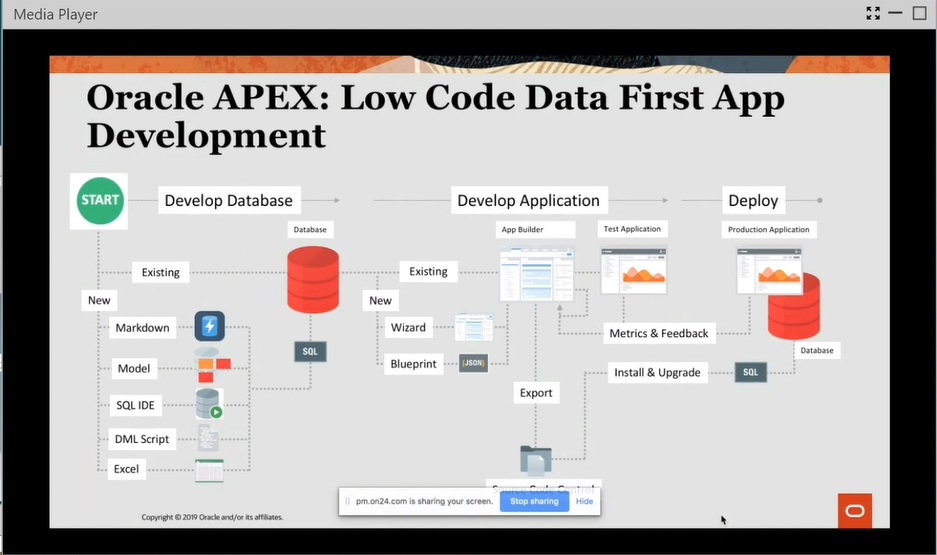
\includegraphics[width=10cm\textwidth]{figure/low data.jpg}
    \end{center}
\section{Mengelola Data Dalam Spreadsheet Menantang}
\begin{enumerate}
    \item Memvalidasi Data Secara Manual Dan Rawan Kesalahan
\item Integritas Data -Tidak Dapat Menjamin Keakuratan Data pada Lingkungan Multi-Pengguna.
\item Keamanan Data Tidak Efektif.
\item Berbagi Data-Excel Lamban Dan Sulit Untuk Dibagikan
\end{enumerate}
\section{Jenis Aplikasi Apa Yang Cocok Untuk Oracle Apex?}
\begin{enumerate}
    \item Large mission-critical apps for thousand of users
    \item Fill in gaps in corporate systems
    \item Streamline Proses Bisnis Yang Sudah Ketinggalan Zaman
    \item Steamline outed business processes
    \item Modernization of legacy systems
    \item Self-service apps for all employees
    \item Customer/Partner-facing portals
    \item proof of concepts
    \item Quick =-win apps (lifespan < a few months
    \item Replacing spreadsheets
\end{enumerate}
\section{Apa Itu Oracle Apex?}
\usepackage{Kerangka kerja pengembangan aplikasi web database-centric.}
\begin{center}
    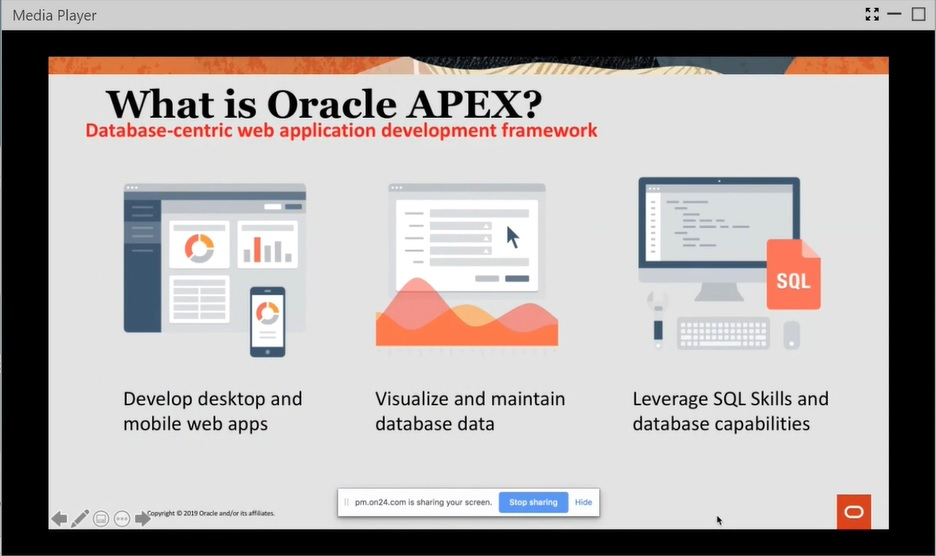
\includegraphics[width=10cm\textwidth]{figure/1.jpg}
    \end{center}
\begin{enumerate}
    \item Mengembangkan Aplikasi Web Desktop Dan Seluler, 
    \item Memvisualisasikan Dan Memelihara Data Basis Data, 
    \item Meningkatkan Keterampilan Sql Dan Kemampuan Basis Data.

\end{enumerate}
\subsection{Oracle Apex: Use Cases}
\subsubsection{	Memodernisasi Formulir Orecle }
\textbf{Fitur}
\begin{enumerate}
    \item Seret daan letakkan file Xls, Csv, Xml, Atau Json
\item Membuat tabel dalam Database Autonomous
\item aplikasi ke tabel baru
\item Buat Aplikasi Berdasarkan Tabel Baru

\end{enumerate}
\textbf{Solusi}
\begin{enumerate}
\item Sumber kebeneran tunggal
\item Kirim URL bukan file
\item Aplikasi yang aman, terukur, multi pengguna
\item Perluasan dengan bagan, kalender, validasi, dan lainnya

\end{enumerate}
\subsubsection{Pengembangan Aplikasi yang Cepat}
\textbf{Fitur}
\begin{enumerate}
    \item Membangun aplikasi dalam beberapa hari / minggu bukan bulan / tahun
\item Gunakan penyihir yang kuat untuk membuat aplikasi berfitur lengkap
\item Mudah dimodifikasi untuk memenuhi perubahan persyaratan
\item  Dengan cepat beralih ke aplikasi yang siap produksi\\
\item Kemampuan kode rendah memungkinkan profesional non-IT juga membangun atau membantu membangun aplikasi\\

\end{enumerate}

\textbf{Solusi}
\begin{enumerate}
    \item Oportunistik
\item Aplikasi taktis sederhana untuk memenuhi kebutuhan mendesak
\item Webify proses kertas
\item Umumnya dikembangkan oleh satu atau dua orang

\end{enumerate}
\subsection{Memperluas Sistem Perusahaan}
\textbf{Fitur}
\begin{enumerate}
    \item  Perluas ERP dan perangkat lunak perusahaan lainnya
    \item Menyediakan dasbor khusus organisasi
    \item Alur kerja yang ditingkatkan
    \item Isi celah
\end{enumerate}
\textbf{Solusi}
\begin{enumerate}
    \item Memenuhi persyaratan non-standar
    \item Optimalkan fungsi bisnis umum
    \item Tingkatkan pengambilan data
    \item Mengintegrasikan sumber data yang berbeda
\end{enumerate}

\Section{Orecle APEX: Distinguishing Characteristic}
	Pengembangan Aplikasi  IDE adalah browser web. Tidak perlu perangkat lunak klien. Aplikasi disimpan pada Database sebagai data meta. Deklaratif – didak ada pembuatan kode, Halaman efisien hanya ada 1 request dan  1 respon pemrosesan data dilakukan dalam database.


\section{Fitur Tanpa Biaya dari Database Orecle}
\textbf{Fitur yang didukung penuh tanpa biaya}
\begin{enumerate}
    \item Beberapa Aplikasi, Pengembang & Pengguna Akhir
\item Tim Dukungan Oracle Khusus
\item 11gr2, 12c, 18c
\item Semua Edisi DB EE, SE2, XE , 
\end{enumerate}


\textbf{Termasuk Dengan Layanan Clound Oracle}
\begin{enumerate}
    \item Database Mandiri 
\item Database Sebagai Layanan
\item Tidak Ada Evaluasi Biaya http: //Apex.Oracle.Com
\end{enumerate}

\textbf{Mudah untuk Diinstal}
\begin{enumerate}
    \item Termasuk secara default dengan semua edisi database Orecle
    \item Unduh Formuli terbaru http://apex.orecle.com/otp

\end{enumerate}



\Section{Opsi Opsi Deveploment / Penyebaran}
\textbf{Lokal}
\begin{enumerate}
    \item Instal Pada Laptop Yang Berdiri Sendiri Menggunakan Edisi Oracle Express Edition (Xe) Atau Database Lengkap.
\item Cukup Tingkatkan Apex Ke Versi Yang Diperlukan.
\item Dapat Bekerja Sepenuhnya Tanpa Terputus.
\end{enumerate} 


\textbf{Di Tempat}
\begin{enumerate}
    \item Biasanya Dijalankan Oleh Departemen TI
\item TI Umumnya Adalah Layanan Operasi Produksi, Dan Penyedia Layanan
\item Departemen Yang Bertanggung Jawab Untuk Pengembangan Aplikasi.
\item Fitur Tanpa Biaya Dari Database Oracle
\end{enumerate}


\textbf{Cloud}
\begin{enumerate}
    \item  Menyebarkan aplikasi internet
\item Dihapus untuk pengembangan aplikasi yang cepat, penerimaan pengguna dan pelatihan\\
\item Prototyping dan Proof-of-Concept
\item Perusahaan konsultan mengembangkan untuk penempatan premis pelanggan
\end{enumerate}

\section{Mesin Virtual Basis Data Tunggal / Beberapa Ruang Kerja}

\begin{center}
    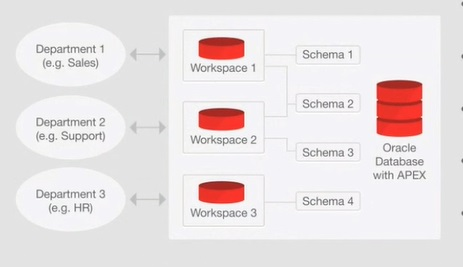
\includegraphics[width=10cm\textwidth]{figure/3.jpg}
    
\end{center}

\begin{enumerate}
    \item Ruang kerja yang digunakan untuk mendefinisikan definisi aplikasi / Skema menyimpan data
    \item Hubungan Banyak-ke-banyak antara Ruang Kerja dan Skema
    \item Instance Administrator mengelola lingkungan dan akses skema
    \item Departemen dapat meminta lebih banyak ruang, dan akses ke skema baru
    \item Misalnya, layanan hanya-internal Oracle http://apex.oraclecorp.com memiliki lebih dari 5.000 Workspaces, yang mencakup setiap lini bisnis di Oracle

\end{enumerate}
\section{Community}
\begin{center}
    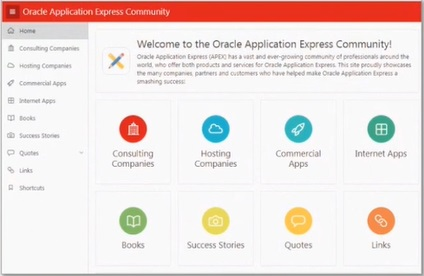
\includegraphics[width=10cm\textwidth]{figure/Community.jpg}
\end{center}
\begin{enumerate}
    \item Lebih dari 500,00 pengembang di seluruh dunia
    \item Diperkirakan dari permintaan dukungan, unduhan, konferensi, aktivitas forum diskusi
    \item Lebih dari 100 blogger aktif http: //odtug.com/apex
    \item http://apex.oralce.com/komunitas konsultasi masyarakat, buku, kesuksesan, cerita, kutipan, aplikasi komersial

\end{enumerate}

\Section{Pendidikan}
\usepackage{Apakah Anda Seorang Siswa Atau Guru SQL, Database Relasional, atau Pengembangan Aplikasi, Anda Dapat Menggunakan Oracle Apex Untuk Sangat Memperkaya Pengalaman Pendidikan Anda?}

\Section{Sertifikasi APEX}
\usepackage{Setelah Anda Mahir Mengembangkan Aplikasi APEX, Anda Dapat Mengikuti Ujian Sertifikasi Oracle Menjadi Aplikasi Oracle Express 18: Profesional Bersertifikat Pengembang.Menonjol Di Antara Rekan-Rekan Anda, Dan Buktikan Kepada Semua Orang Bahwa Anda Tahu Cara Membangun Aplikasi Yang Kuat Dengan Menggunakan Apex.}

\Section{Kurikulum Gratisan Oracle Apex}
\begin{enumerate}
    \item 	Pelajar, Dan Panduan Praktikum Di Laboratorium
\item Total 16 Pelajaran Dan 15 Tangan Di Laboratorium
\item PPT, PDF, Sumber, Dan File Lab
\item Lab / Demo Dapat Dilakukan Pada: Contoh Akademi Oracle
\end{enumerate}
\Section{Gambaran Umum }
\usepackage{Lab Ini Menuntun Anda Saat Mengunggah Spreadsheet Ke Tabel Database Oracle, Lalu Membuat Aplikasi Berdasarkan Tabel Baru Ini.  Anda Kemudian Akan Bermain Dengan Laporan Interaktif Dan Meningkatkan Formulir Terlampir.  Terakhir, Anda Akan Menambahkan Halaman Kalender Dan Kemudian Menautkannya Ke Halaman Formulir Yang Ada.  Alih-Alih Mencoba Mengirim Surel Spreadsheet Untuk Mengumpulkan Informasi Dari Orang Yang Berbeda, Cukup Buat Aplikasi Dalam Hitungan Menit, Dan Kirim Surel URL.  Spreadsheet Sumber-Kebenaran-Tunggal, Multi-Pengguna, Aman, Dan Mudah Tersiram Ini!  Aplikasi Scren Jadi Lebih Baik}
\section{Memulai Orecle Apex}
\usepackage{Langkah 1.1:}
\begin{enumerate}
    \item Buka link https://apex.orecle.com
    \item Klik Get Started for Free
    \itemKlik Reques a Free Workspace
    \item Masukkan data sesuai perintah 
    \item Setelah semua terisi dan klik Next
    \item Cek Email anda.dan buka email dari oracley
    \item Klik Create Workspace
    \item Klik Continue to Log in Screen
    \item Lalu ubah password anda\\

\end{enumerate}
\begin{center}
    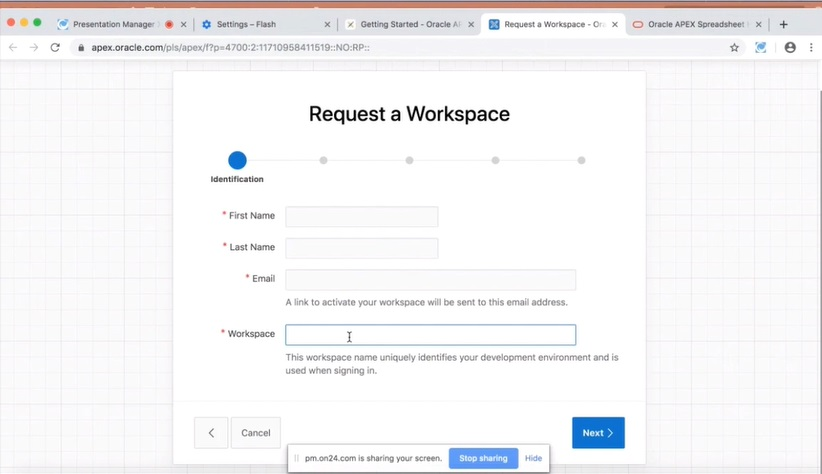
\includegraphics[width=10cm\textwidth]{figure/request.jpg}
\end{center}
\Section{Langkah 2.1 Masuk}
\begin{enumerate}
    \item . Masuk Ke Ruang Kerja Anda Di Http://Apex.Oracle.Com
\item Klik Pembuat Aplikasi Klik Buat Aplikasi Baru
\end{enumerate}
\Section{Langkah 2.3 - Memuat Data Sampel}
\begin{enumerate}
    \item 	Klik Salin Dan Tempel
    \item Klik Selanjutnya\\
\end{enumerate}

\Section{Latihan 2.5 Memverifikasi Catatan Dimuat}
\begin{enumerate}
    \item Centang Bahwa 73 Baris Dimuat
    \item Klik Terus Untuk Membuat Aplikasi Wizard

\end{enumerate}

\Section{Langkah 2.6 - Memberi Nama Aplikasi}
\begin{enumerate}
    \item Nama Enter {App From A Spreadsheet}
	\item Berikutnya Ke Fitur, Klik Centang Semua\\

\end{enumerate}
\Section{Langkah 2.7- Buat Aplikasi}
\begin{enumerate}
    \item Klik Buat Aplikasi\\
\end{enumerate}
\Section{Langkah 2.8- App In Page Desaigner}
\begin{enumerate}
    \item Di Aplikasi Baru Kamu Akan Ditampilkan Desainer
    \item Klik Run Aplikasi\\

\end{enumerate}
\Section{Langkah 2.9- Runrime Aplikasi}
\begin{enumerate}
    \item Masukkan Kredensial Pengguna Anda
    \item Bermain-Main Dengan Aplikasi Baru Anda\\

\end{enumerate}

\Section{Langkah 3.1-  Urutkan Laporan Interaktif}
\begin{enumerate}
    \item Klik Spreadsheet
    \item Clik Actions, Select Data, Select Sort
    \item Untuk 1, Select Start Datte; Untuk 2, Select End Date; Clik Apply
\item Menggunakan Lingkungan Runtime
\item Memperbaiki Laporan Dan Formulir\\

\end{enumerate}

\Section{Langkah 3.2- Menambahkan Komputasi}
\begin{enumerate}
    \item Klik Actions, Pilih Data, Pilih Compute
\item Column Label Masuk Bugget V Cost
\item Format Maskpilih 5,243,10
\item Masukkan Ekspresi Komputasi I-H
\item Klik Apply\\

\end{enumerate}

\Section{Langkah 3.3 “Menambahkan Sebuah Grafik”}
\begin{enumerate}
    \item Klik “Action”, Dan Pilih “Chart”
    \item Label Pilih “**Budget V Cost”
    \item Fungsi Pilih “ Sum”
    \item Sort Pilih “Label-Ascending”
    \item Orientasi Pilih “Horizontal”
    \item Klik “Apply”

\end{enumerate}
\Section{Langkah 3.4 “Menyimpan Laporan”}
\begin{enumerate}
\item Klik”Action”,Pilih “Report”, Pilih”Save Report”
\item Untuk Simpan, Pilih “As Default Report Settings”
\item Tipe Default Laporan, Pilih “ Alternative”
\item Nama, Enter “Data Review”
\item Klik “Apply”\\

\end{enumerate}
\Section{Langkah 3.5 “Batasi Status”}
\begin{enumerate}
    \item Ketika Runtime Environment, Klik “Edit Icon On A Record”
\item Halaman Modal Akan Tampil
\item Pada Developer Toolbar, Klik “Quick Edit”
\item Pada Status Item (Tunggu Sampai Outline Biru Muncul” Lalu Klik Mouse
\item Di Halaman Designer Muncul Dengan Focus Pada Status Item
\item Di Halaman Designer, Dalam Editor Property(Panel Kanan)
\item Di Bawah Daftar Nilai-Nilai, Untuk Type Pilih “SQL Query”
\item Lanjutkan Ke SQL Query, Klik “Code Editor”\\

\end{enumerate}

\Section{Langkah 3.5 C" Membatasi Status (Restrict The Status"}
\begin{enumerate}
    \item Dalam Kode Masukkan Seperti Ini
Select Distinct Status D, Status R From Spreadsheet Order By 1
\item Klik Validate
\item Klik Ok
\item Untuk Menampilkan Nilai Ekstra Pilih No
\item Menampilkan Nilai Null Pilih –Select Status-
\item Klik Save (Pada Toolbar Top Right)\\

\end{enumerate}
\Section{Langkah 3.6 "Menjalankan Apllikasi (Run Apllikasi)"
}
\begin{enumerate}
    \item Arahkan Navigasi Ke Runtime Environment
    \item Refresh Browser
    \item Edit Record
    \item Klik Status\\

\end{enumerate}

\Section{Langkah 4.1 "Tambah Kalender (Add A Calender)"}
\begin{enumerate}
    \item Arahkan Navigasi Kembali Ke Development Environtment
    \item Pada Aplikasi Builder, Arahkan Pada Home Page
    \item Klik Create Page\\

\end{enumerate}

\Section{Langkah 4.1b"Tambahkan Kalender"}
\begin{enumerate}
    \item Klik Kalender
    \item Nomor Halaman, Masukkan Kalender
    \item Remah Roti, Pilih Remah Roti
    \item Klik Selanjutnya\\

\end{enumerate}

\Section{Langkah 4.1c - Tambahkan Kalender}
\begin{enumerate}
    \item Preferensi Navigasi, Klik Buat Entri Menu Navigasi Baru
    \item Klik Selanjutnya
    \item Tabel / Nama Tampilan, Pilih Spreadsheet (Tabel)
    \item Klik Selanjutnya

\end{enumerate}

\Section{Langkah 4.1d  "Tambahkan Kalender"}
\begin{enumerate}
\item Kolom Tampilan, Pilih TASK_NAME
\item Kolom Tanggal Akhir, Pilih END_DATE
\item Klik Buat

\end{enumerate}
\Section{Langkah 4.2 "Menautkan Kalender Ke Dari"}
\begin{enumerate}
    \item Di Tab Rendering, Di Bawah Kalender, Klik Atribut
    \item Di Editor Properti (Panel Kanan), Klik Lihat / Edit Tautan
    \item Halaman, Pilih 3
    \item Mengatur Item-Nama, Pilih P3_ID; Nilai, Pilih ID
    \item Bersihkan Cache, Masukkan 3
    \item Klik Ok
    \item Klik Simpan Dan Jalankan\\

\end{enumerate}

\section{Pengertian Spreadsheet}
\usepackage{Spreadsheet: Memungkinkan Pengguna Untuk Menyimpan Berbagai Informasi Yang Sangat Lengkap, Pada Setiap Kolomnya Bisa Menyimpan Berbagai Data Informasi Yang Berbeda Dari Informasi Yang Di Perlukan.}\\
\usepackage{App From Spreadsheet Disini Berupa Beberapa Project Dan Nama Tugas Nya Serta Keterangan Lainnya Seperti Tanggal Mulai, Tanggal Selesai, Status, Di Ttd Oleh,Biaya, Budget Tersedia, Dan Lebih Kurangnya Dari Budget.}

\Section{Lampiran Langkah-langkah:}

    \item 1.  Setelah sukses login, klik App Builder

\begin{center}
    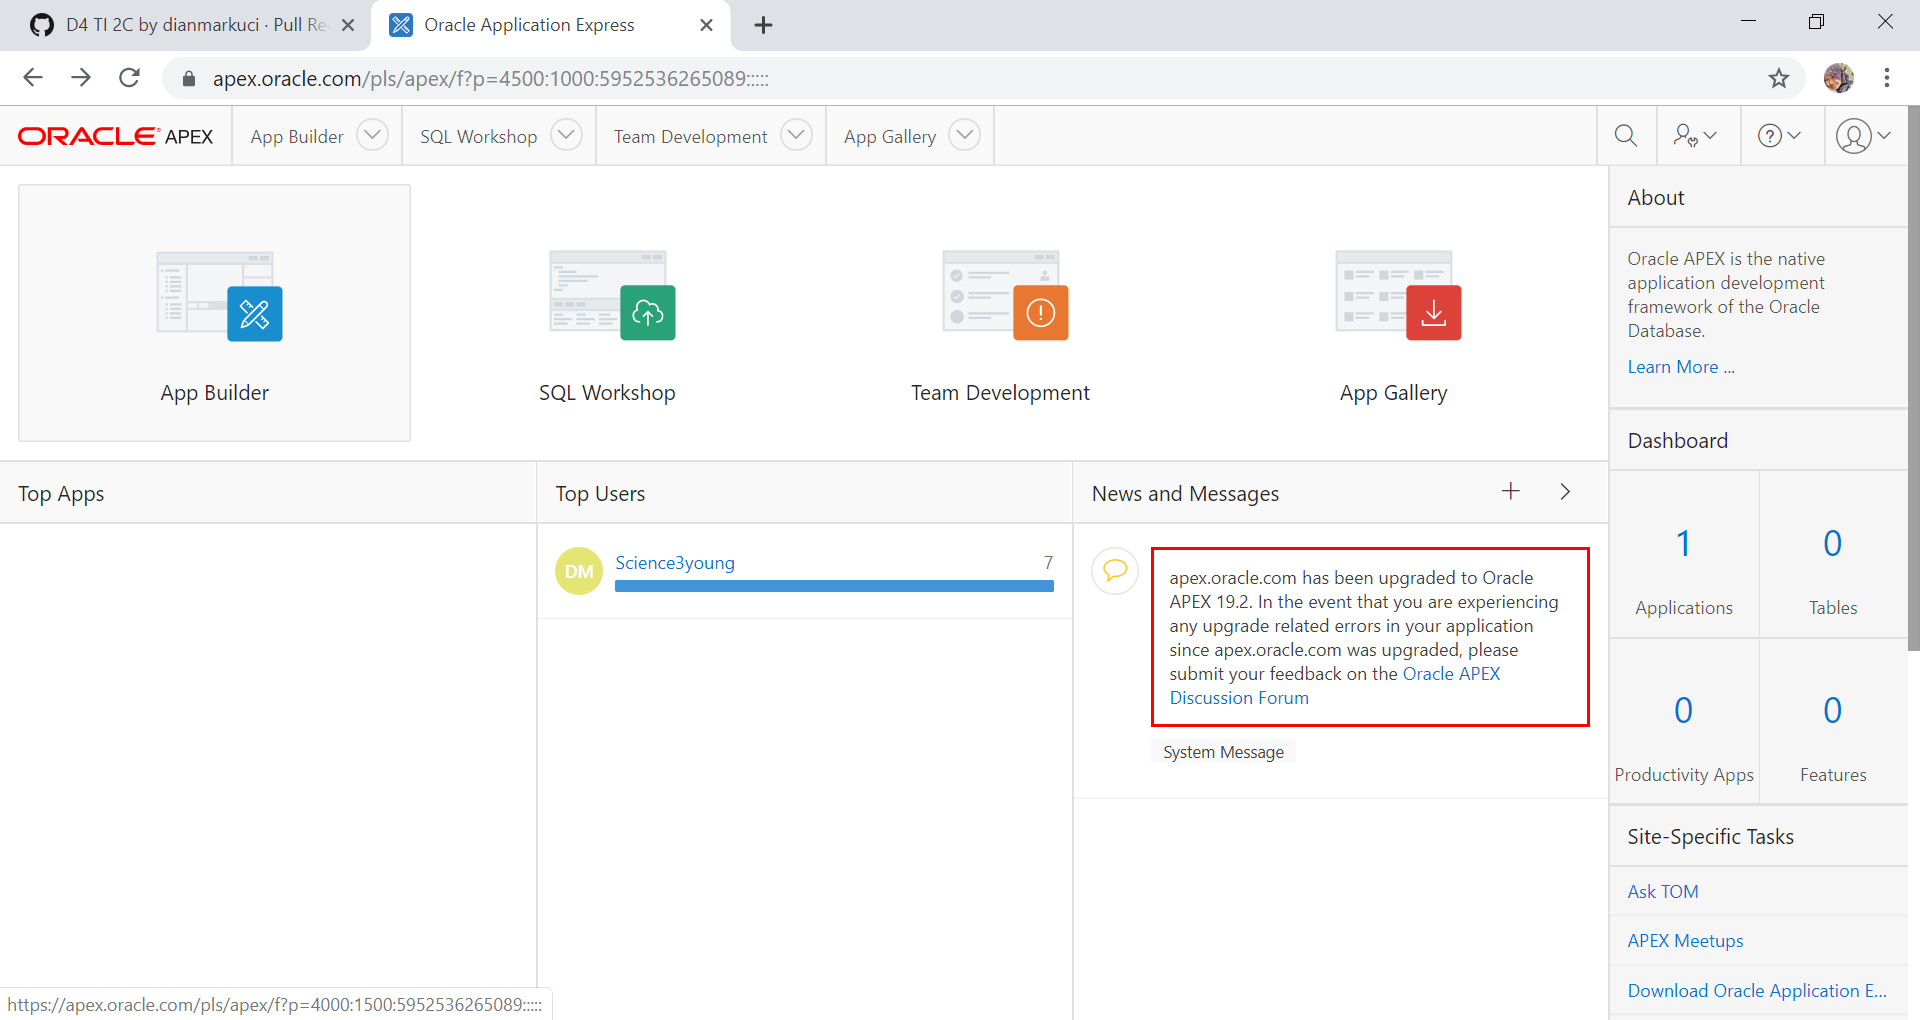
\includegraphics[width=10cm\textwidth]{figure/1.png}
    \end{center}
    
    \item 2. Klik Create

\begin{center}
    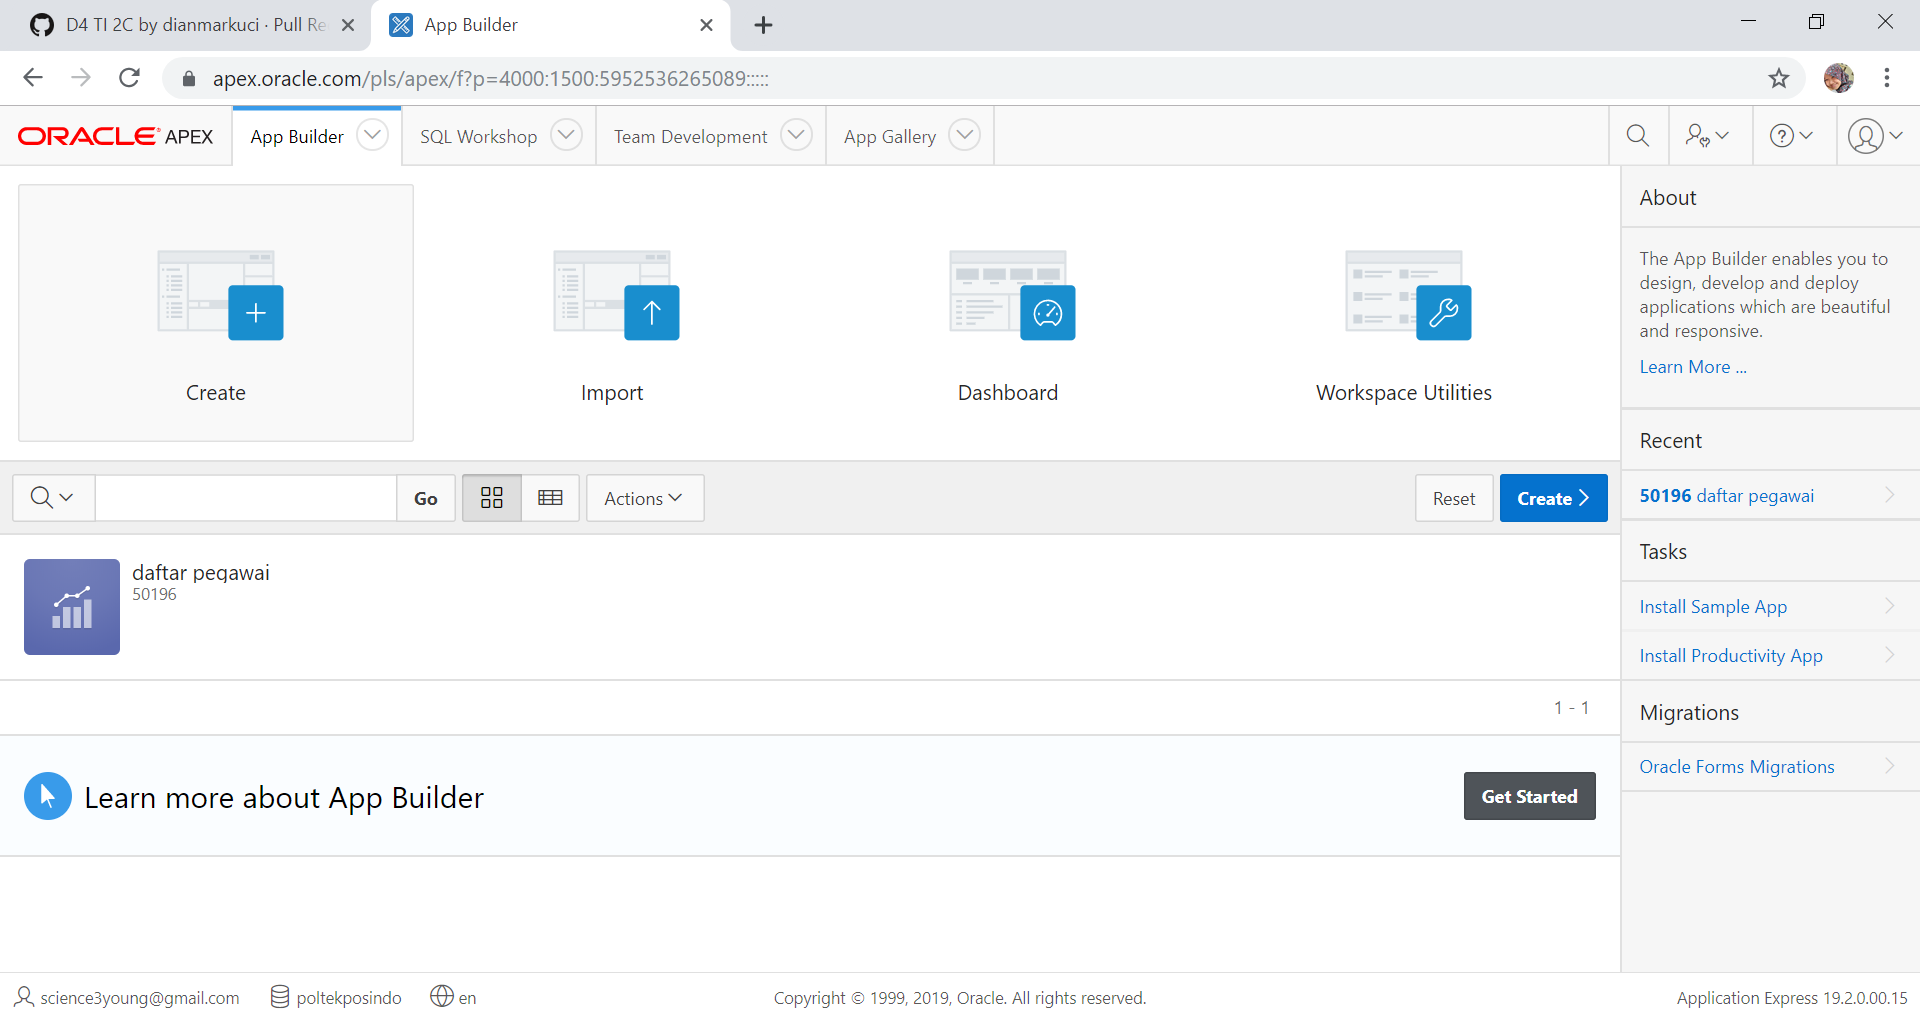
\includegraphics[width=10cm\textwidth]{figure/2.png}
    \end{center}
    

    \item 3. Klik From a File
\begin{center}
    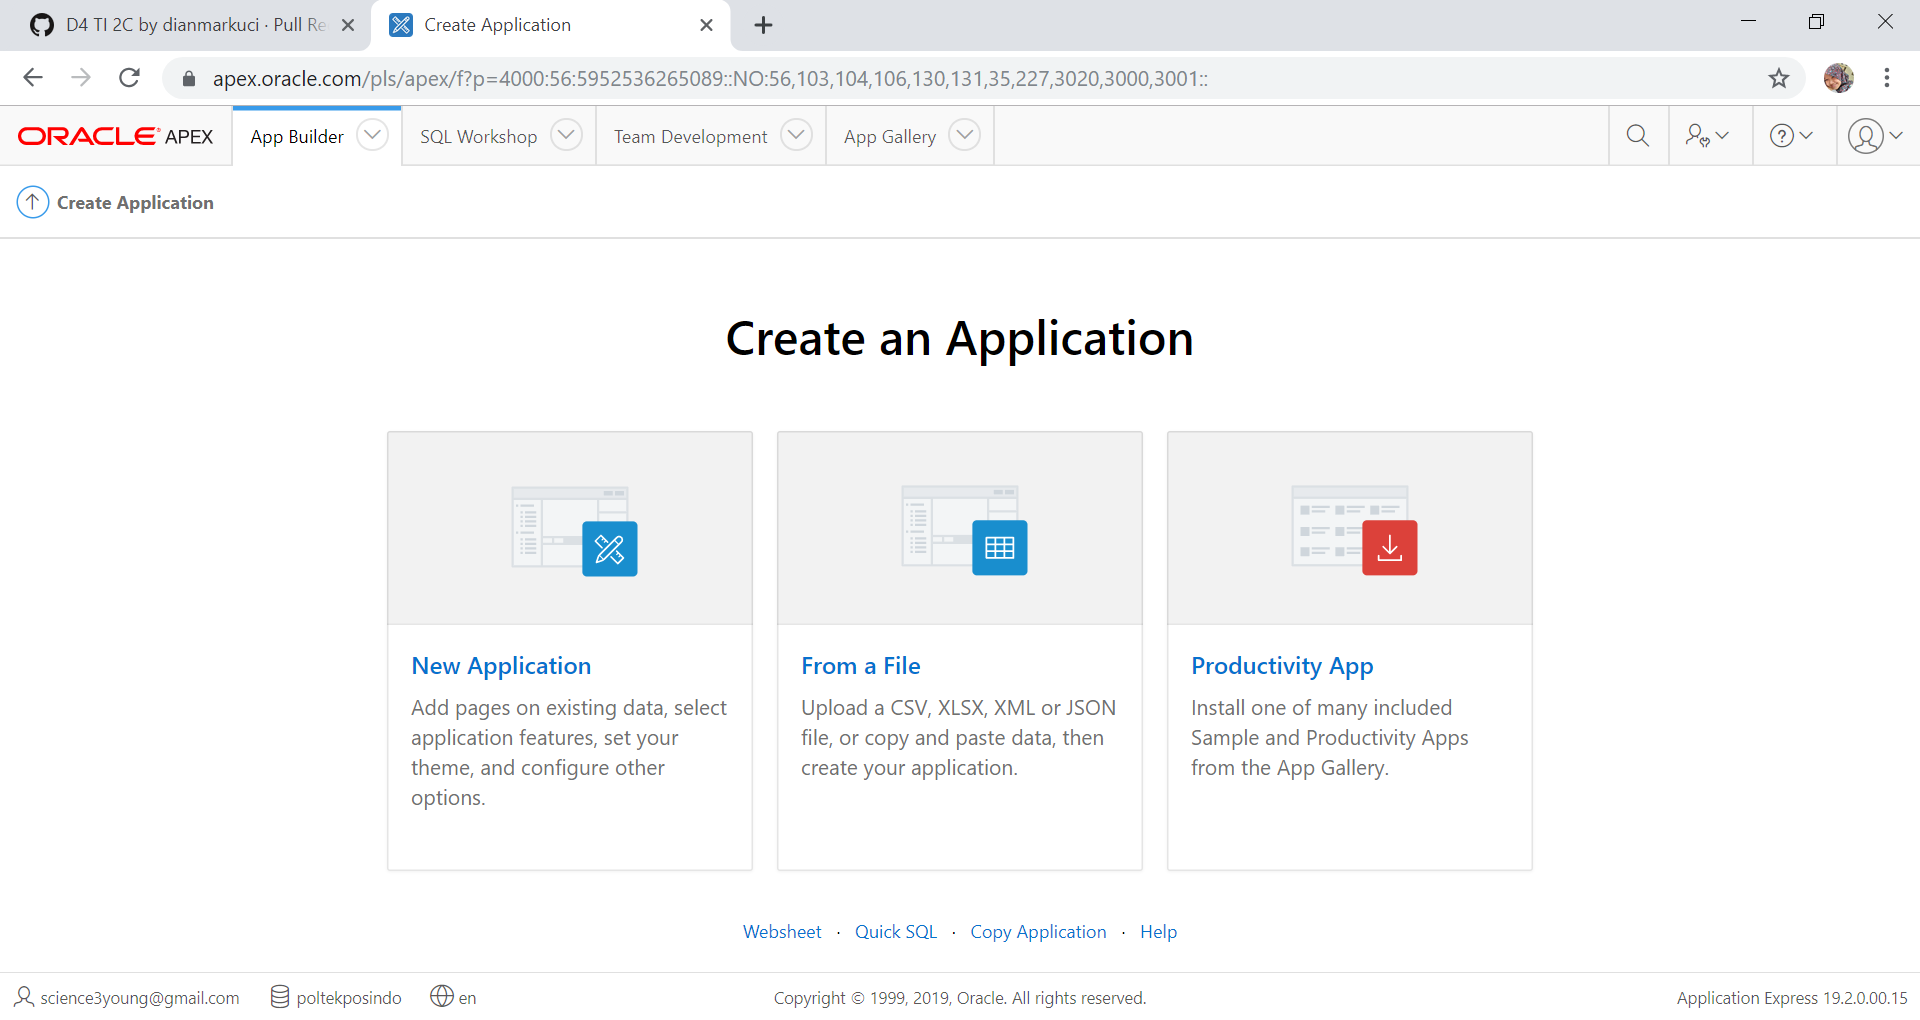
\includegraphics[width=10cm\textwidth]{figure/3.png}
    \end{center}
    
    
    \item 4. Pilih Copy and Paste
\begin{center}
    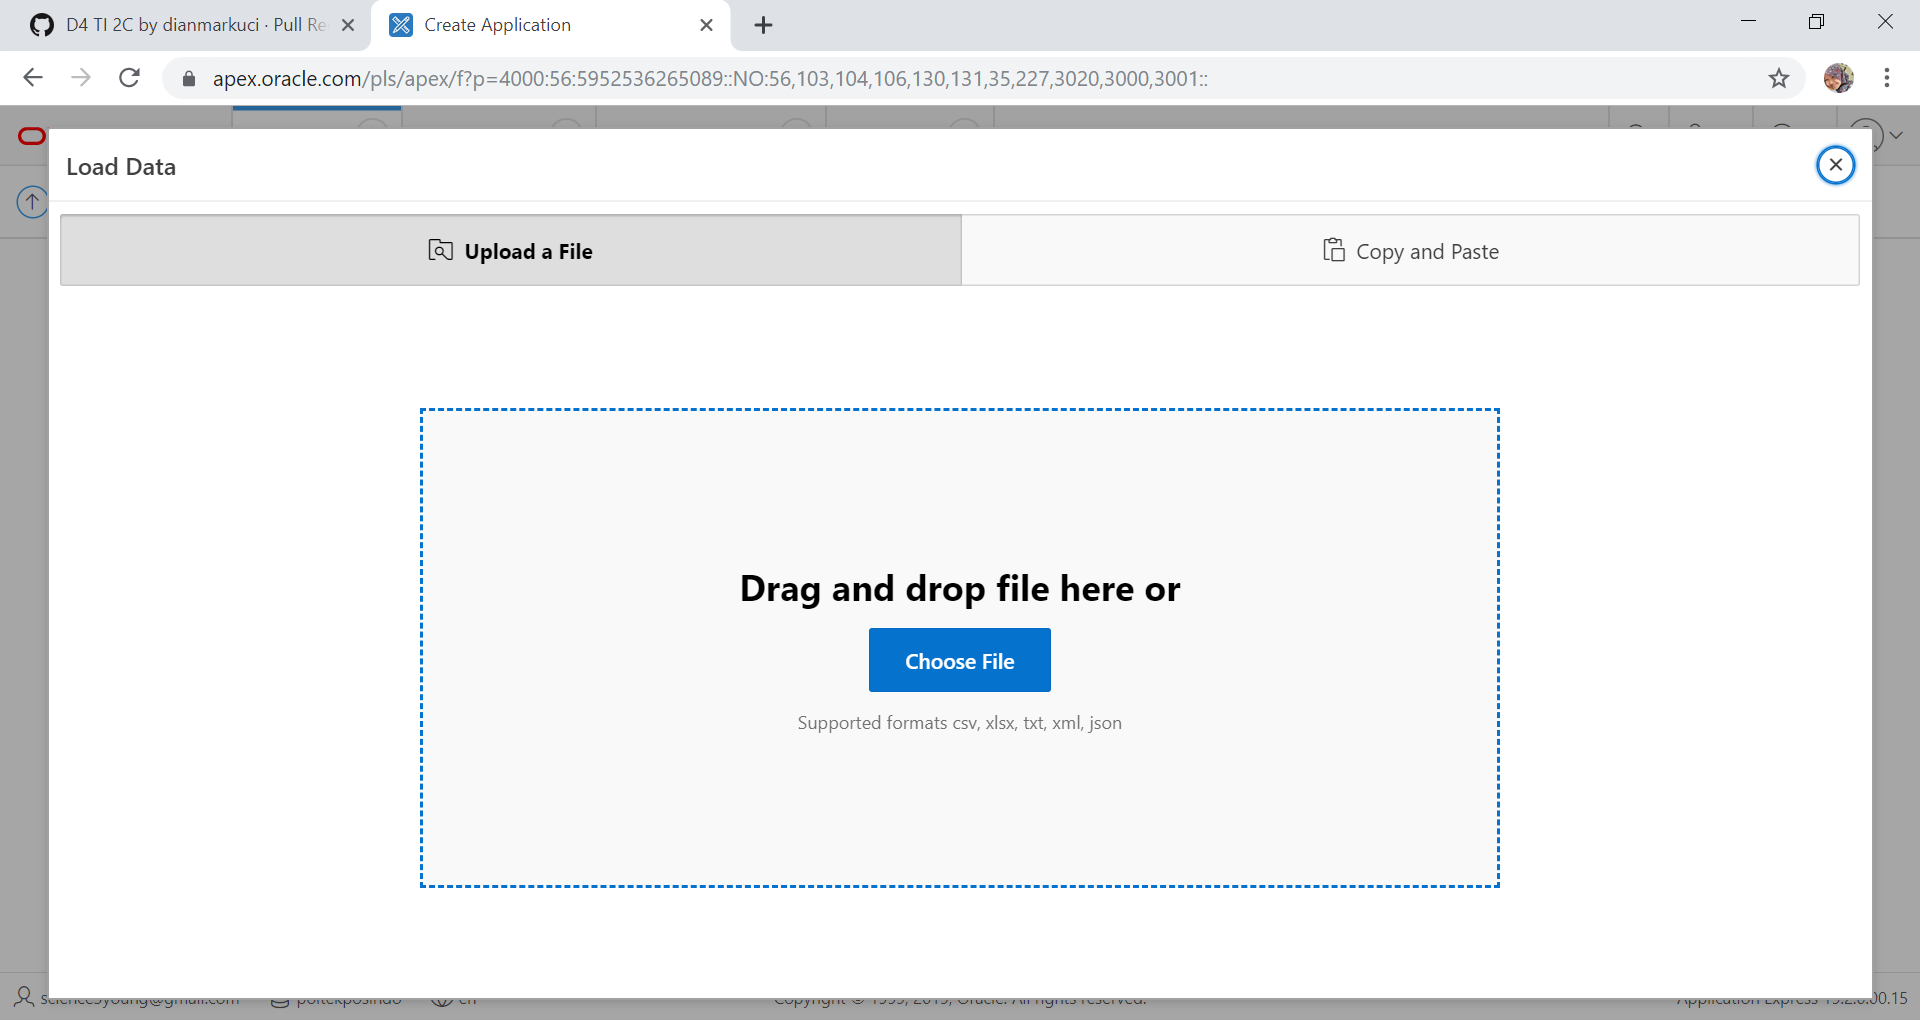
\includegraphics[width=10cm\textwidth]{figure/4.png}
    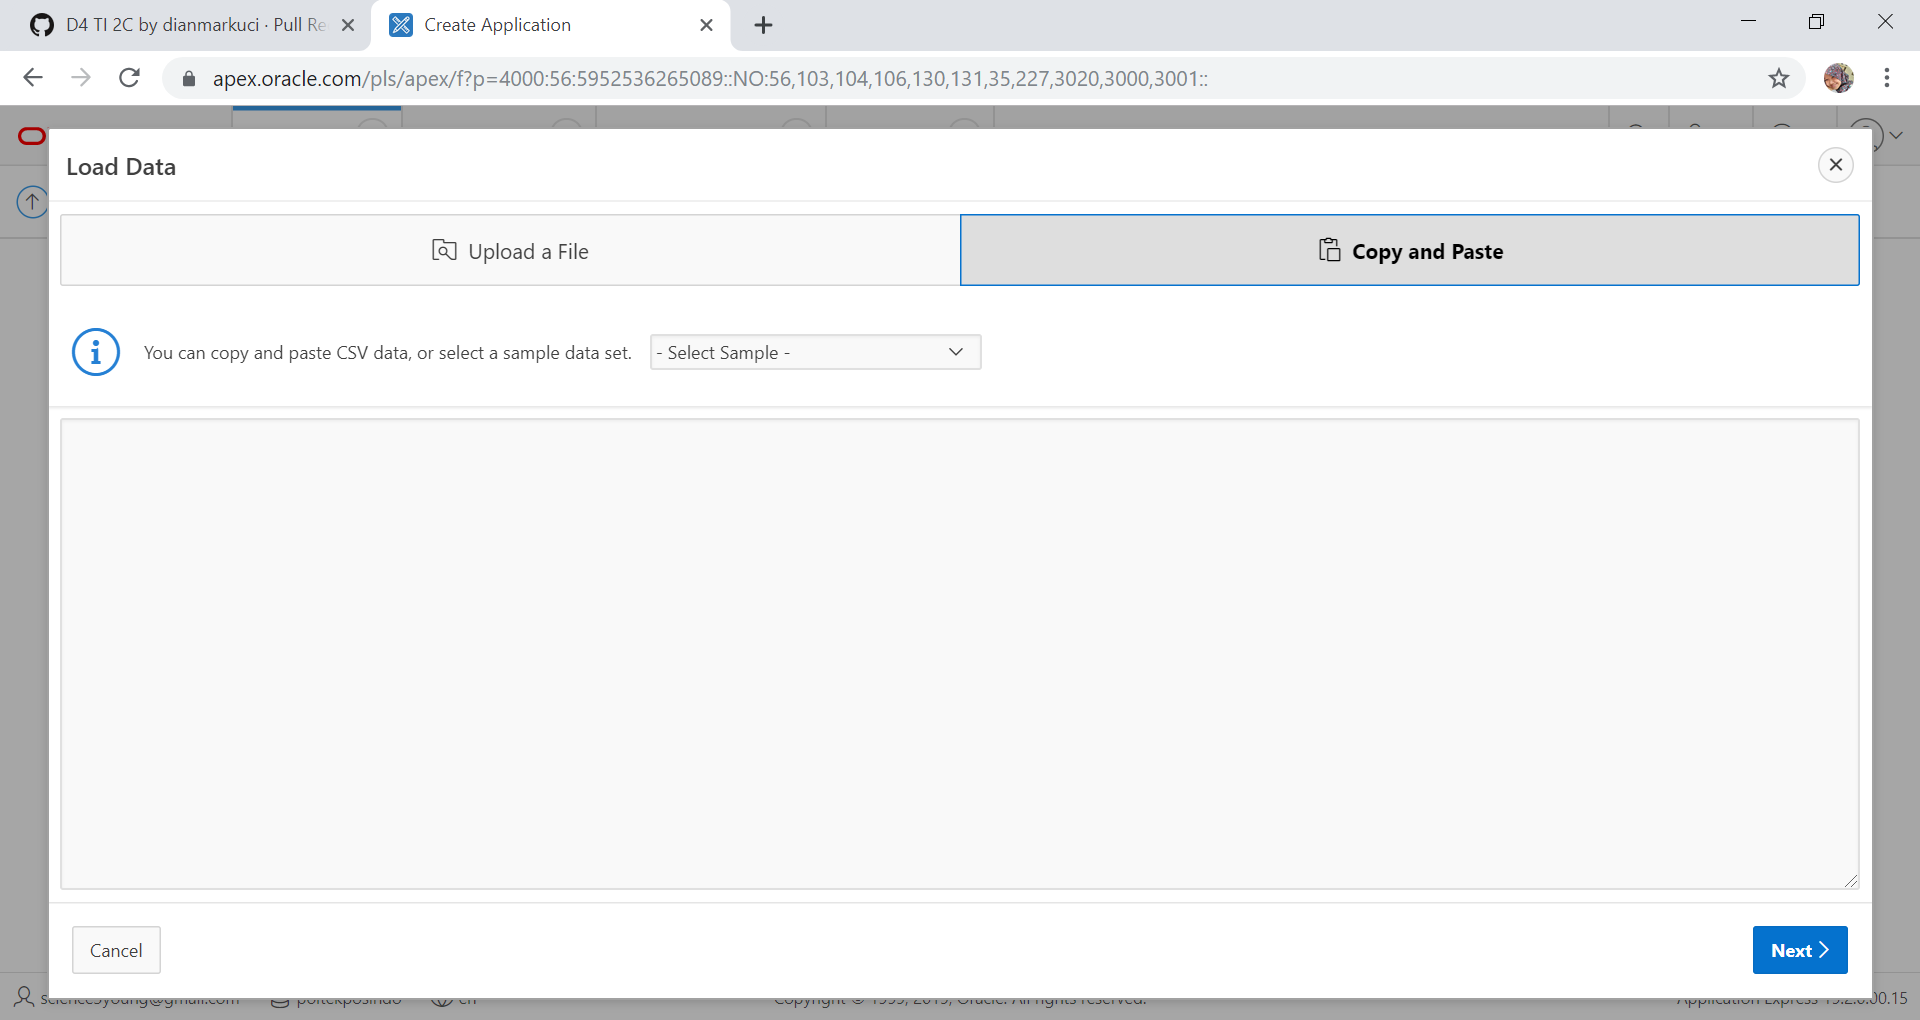
\includegraphics[width=10cm\textwidth]{figure/5.png}
    \end{center}
    
    \item 5. Select Sample lalu pilih projects and Tasks
\begin{center}
    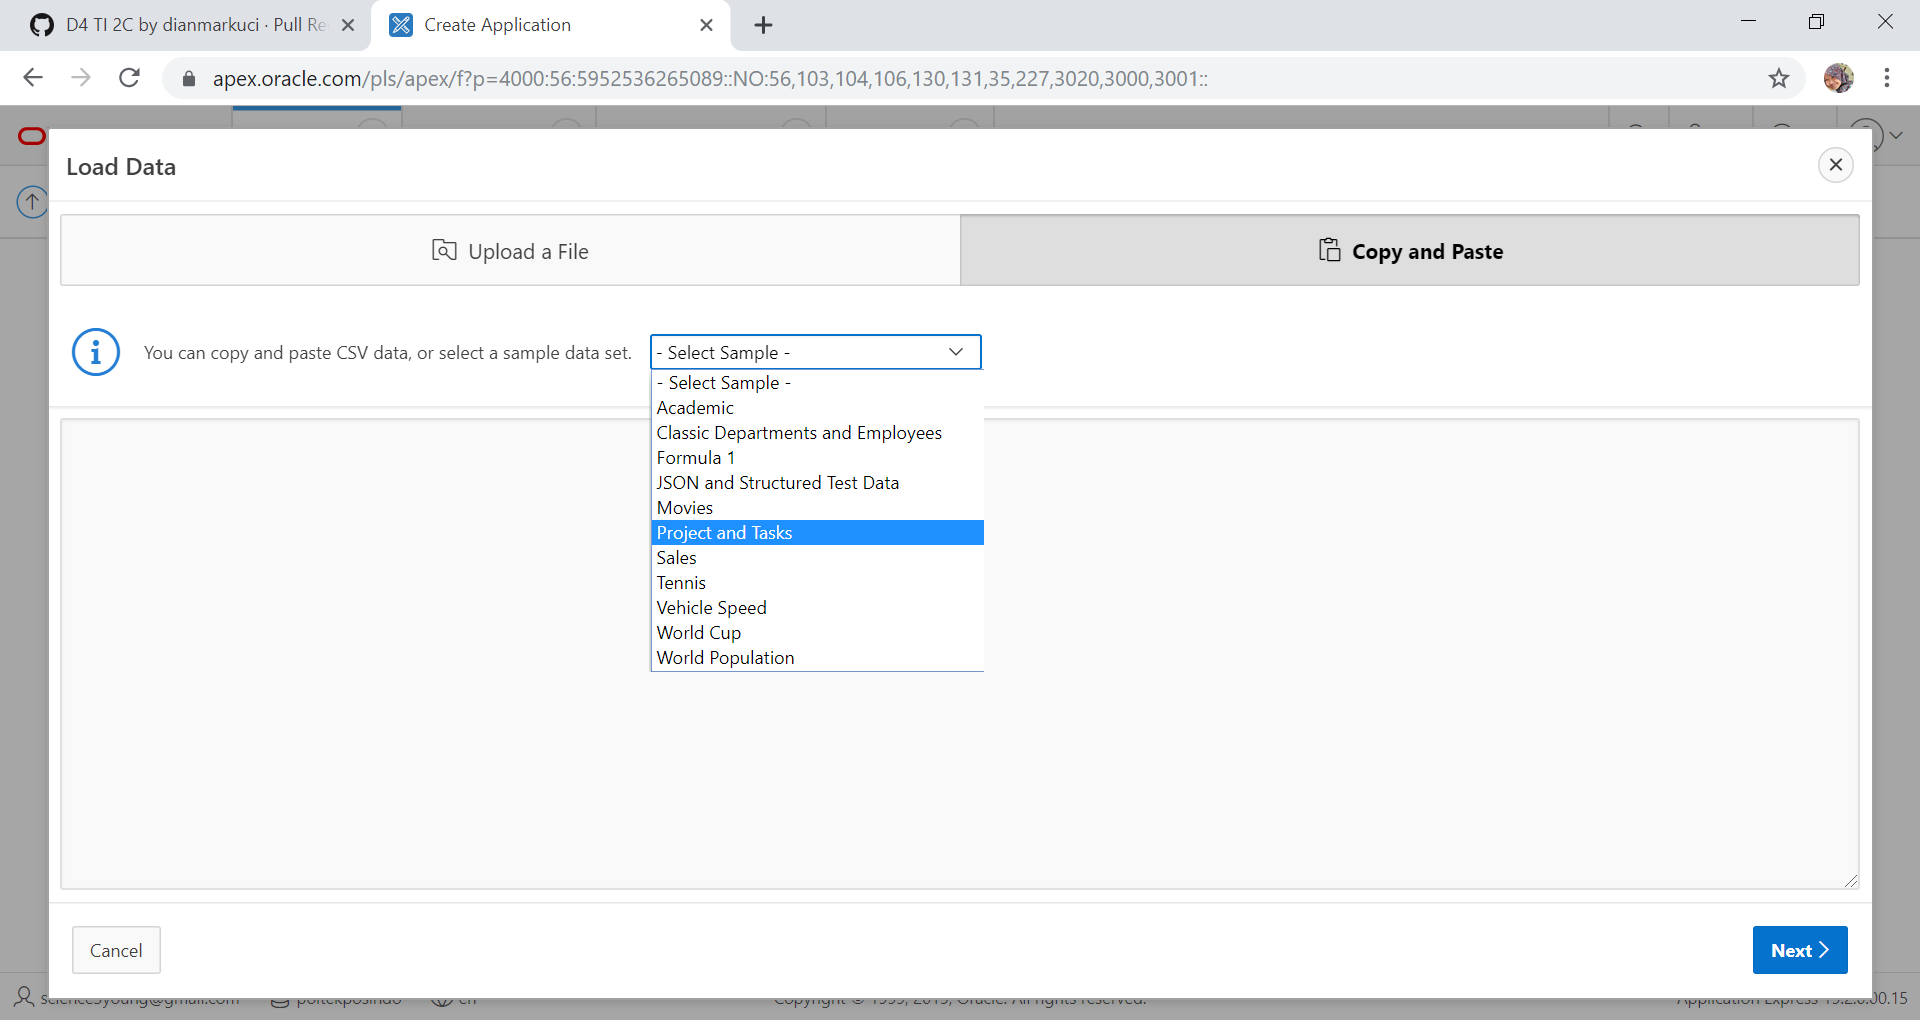
\includegraphics[width=10cm\textwidth]{figure/6.png}
    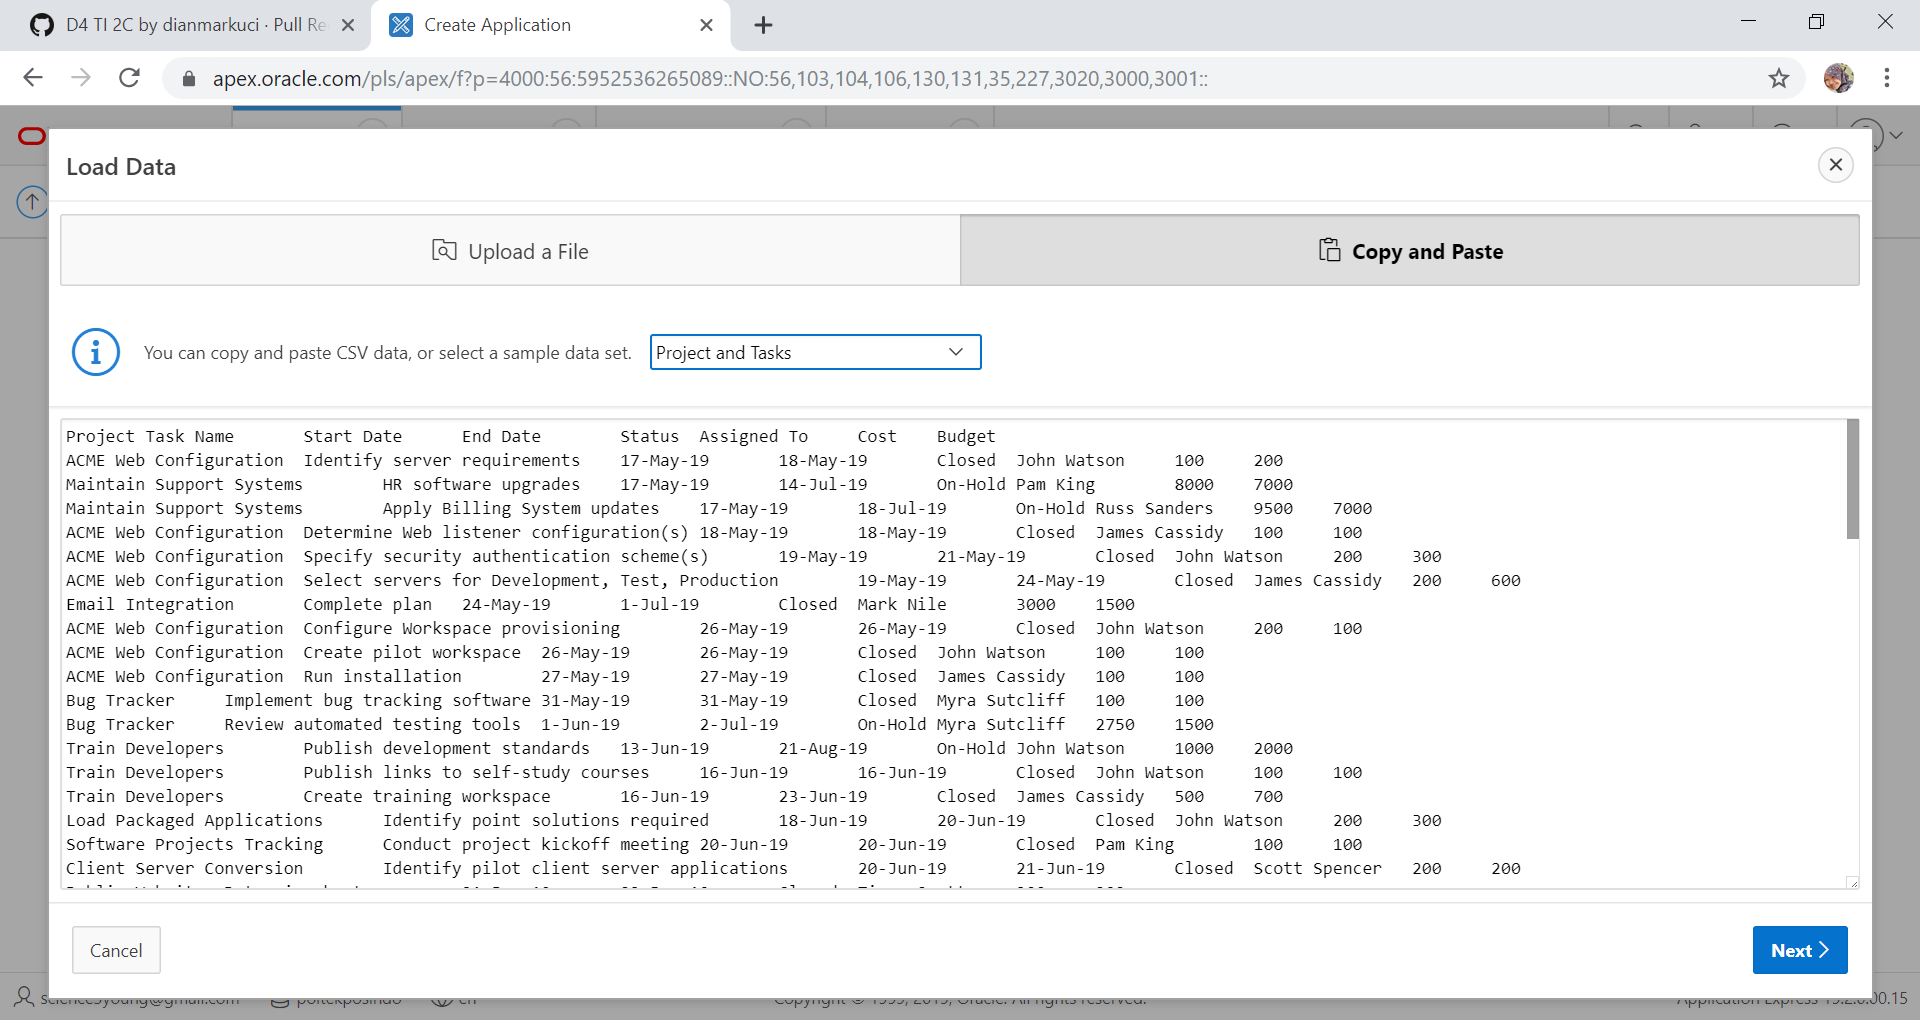
\includegraphics[width=10cm\textwidth]{figure/7.png}
\end{center}
    
    \item 6. Isi table name : spreadsheet
\begin{center}
    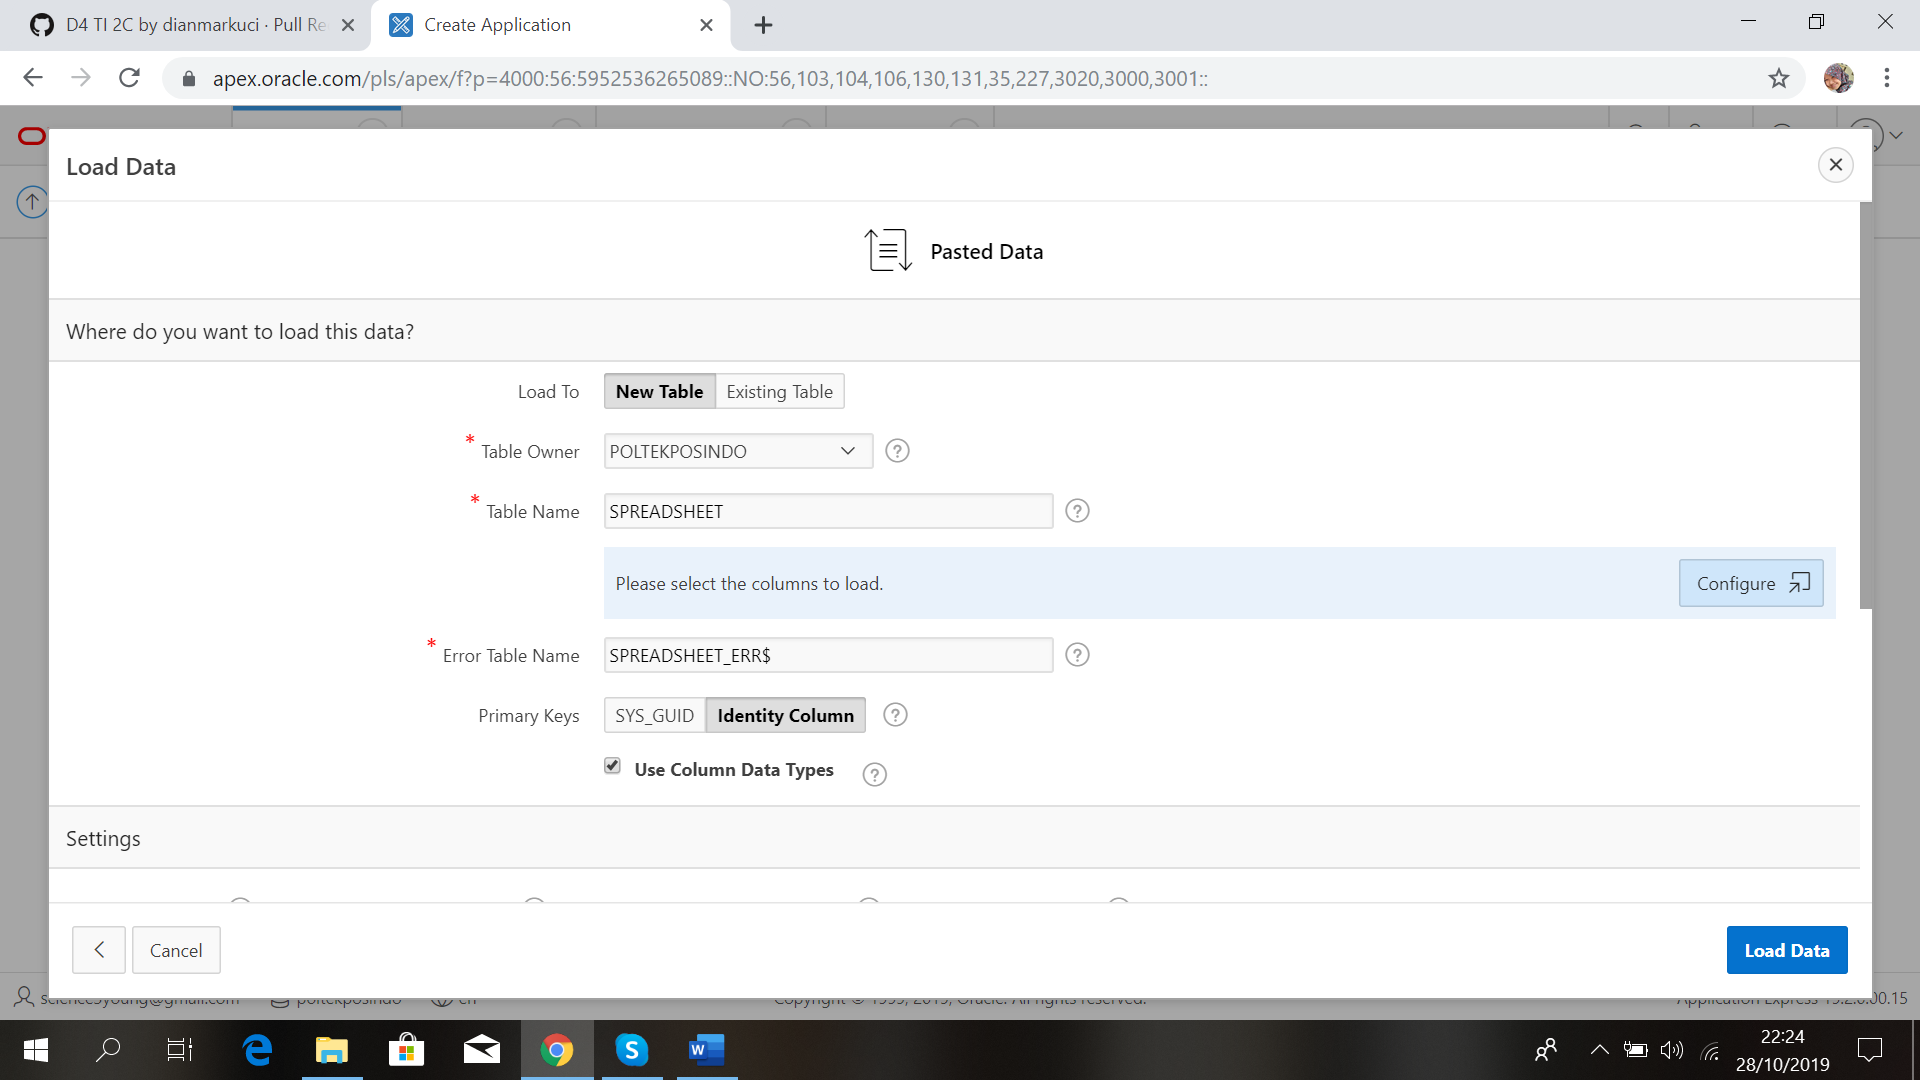
\includegraphics[width=10cm\textwidth]{figure/8.png}
\end{center}

\item 7. table sudah berhasil dibuat
\begin{center}
  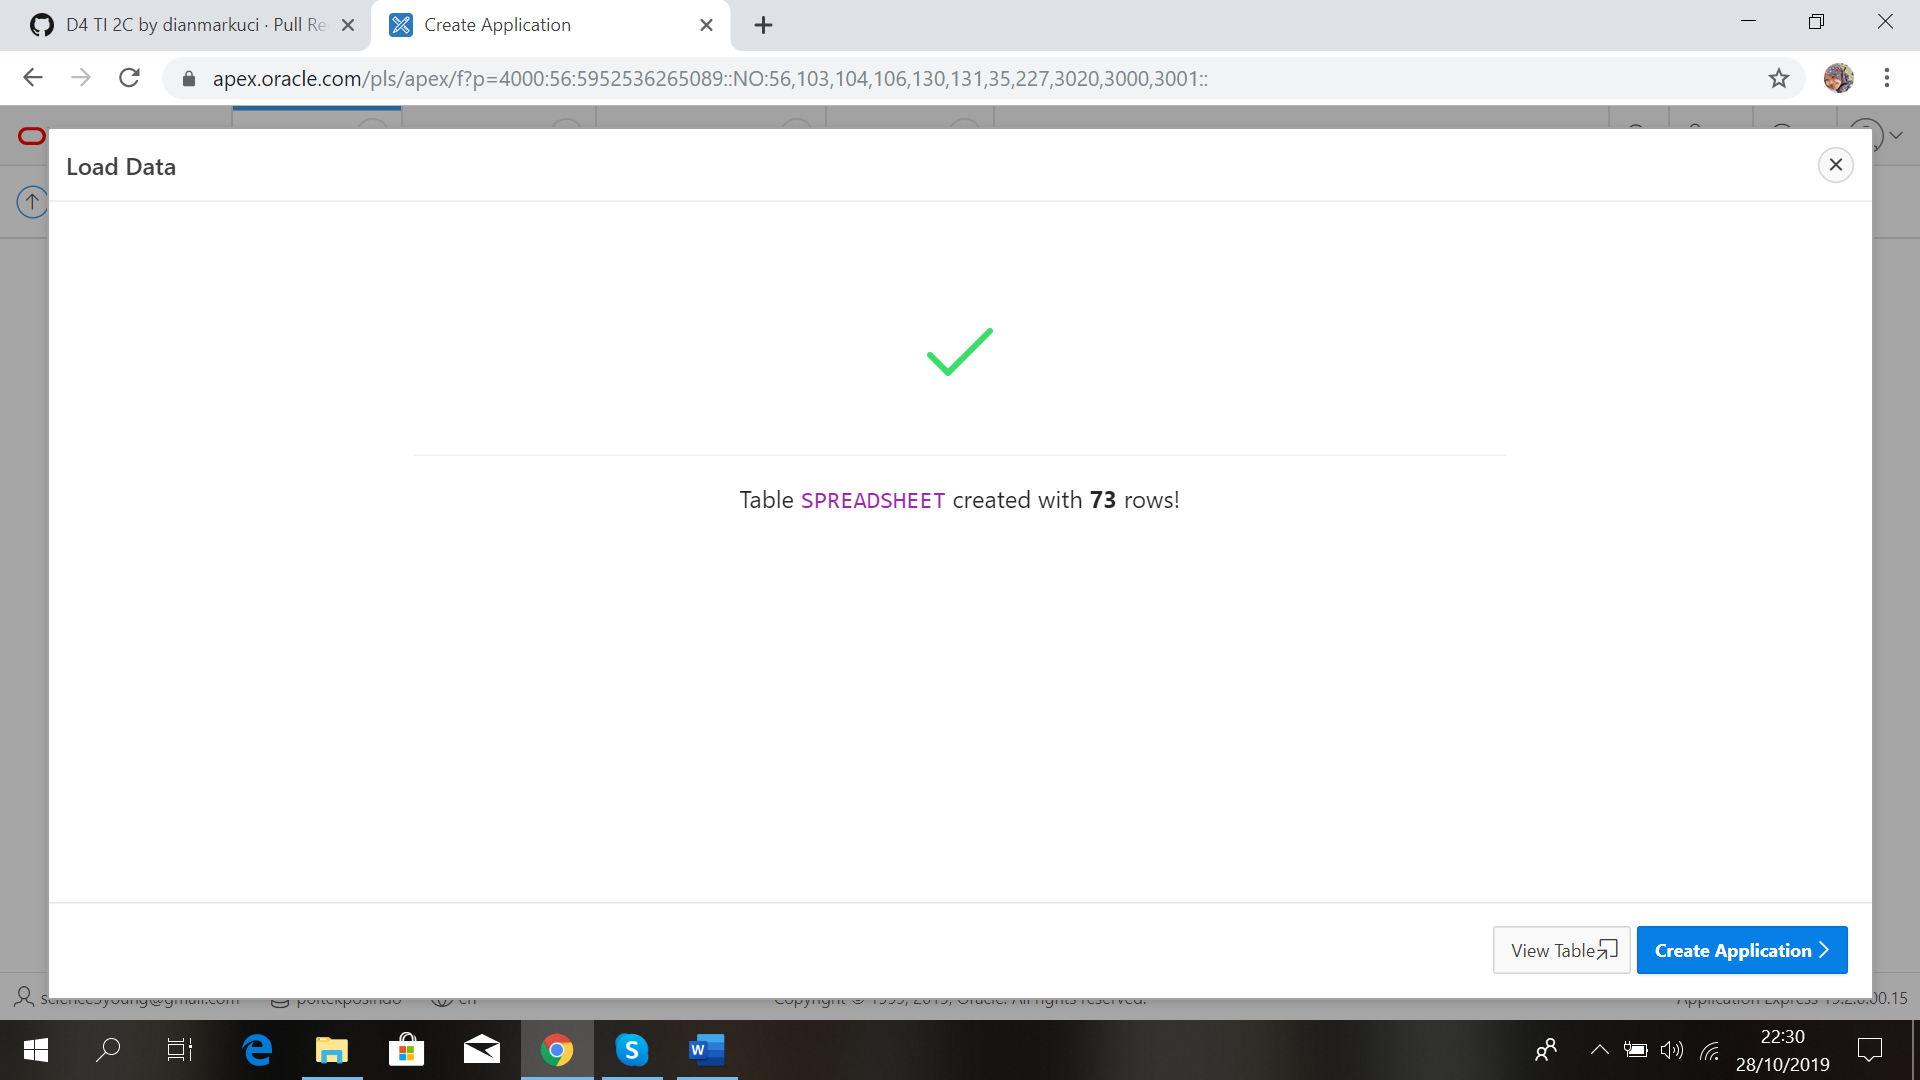
\includegraphics[width=10cm\textwidth]{figure/9.png}
\end{center}
   
\item 8. Create an application
\begin{center}
  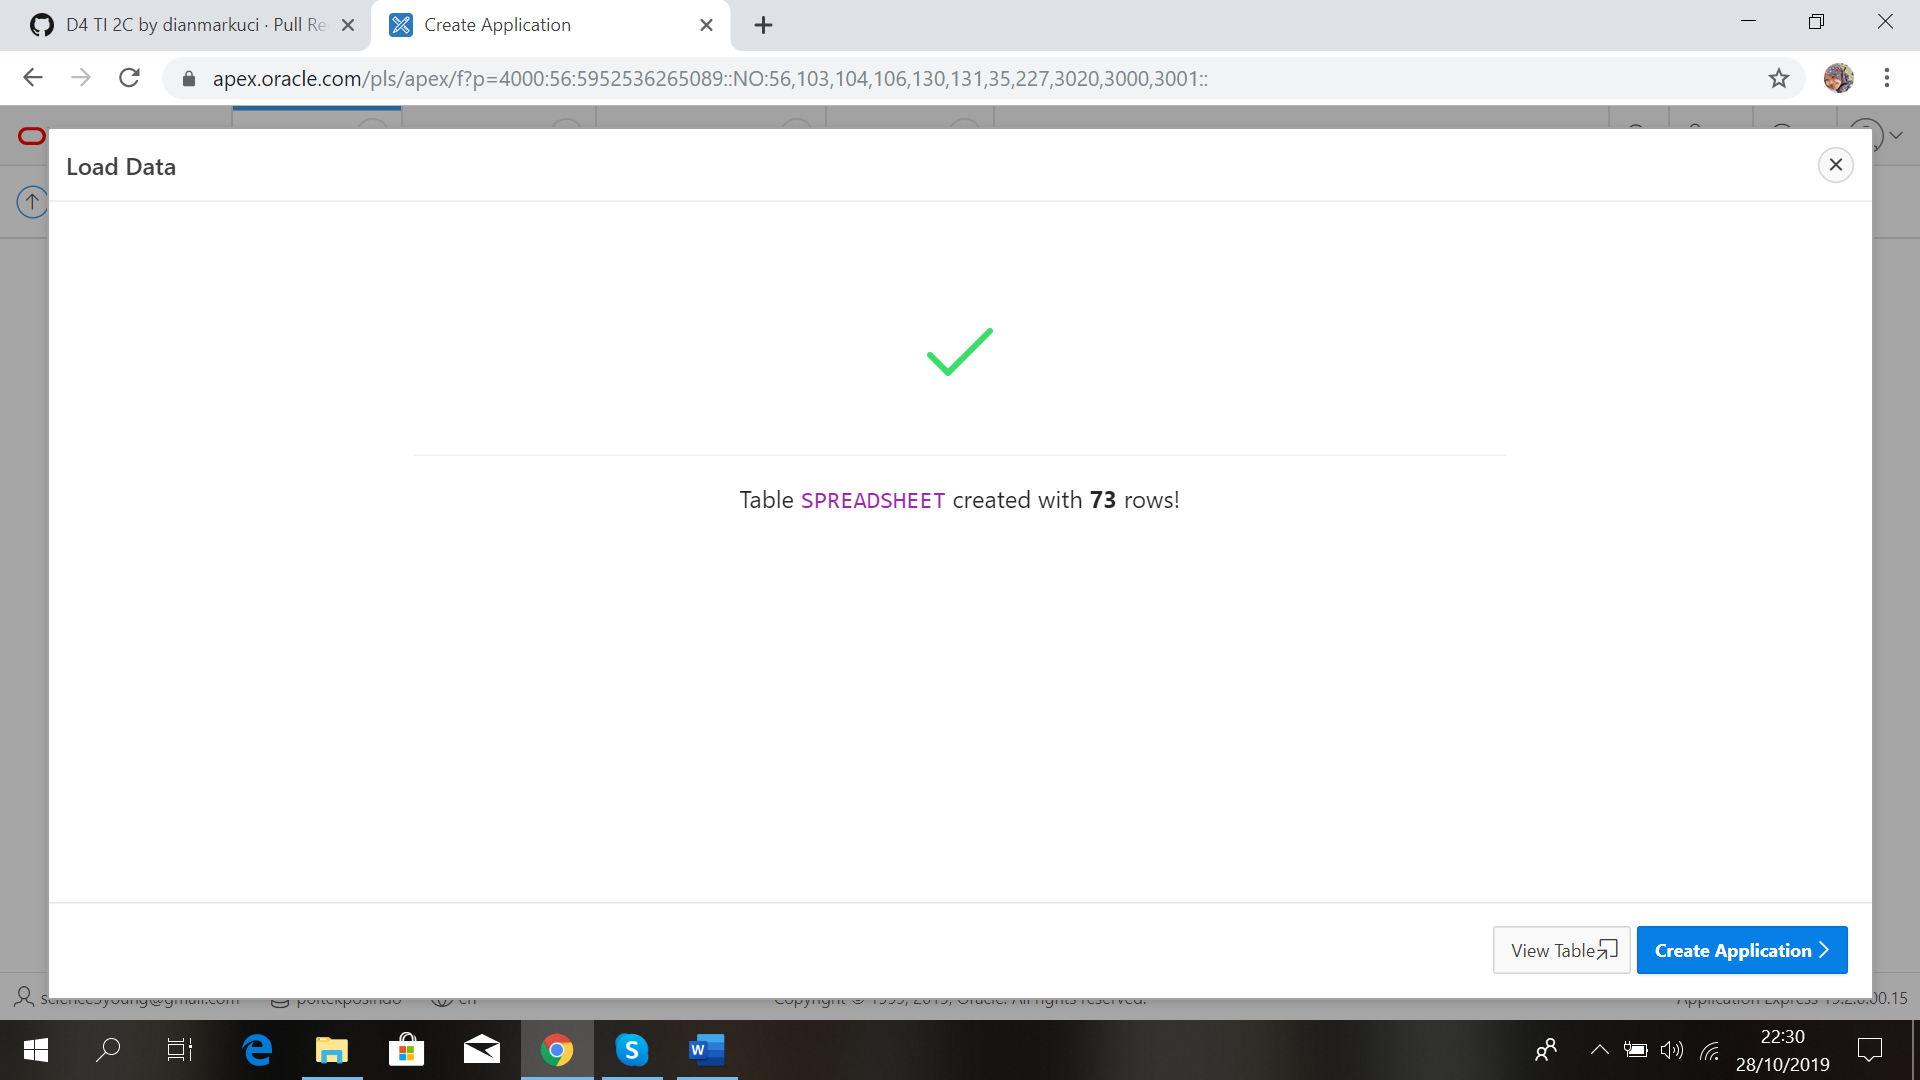
\includegraphics[width=10cm\textwidth]{figure/10.png}
  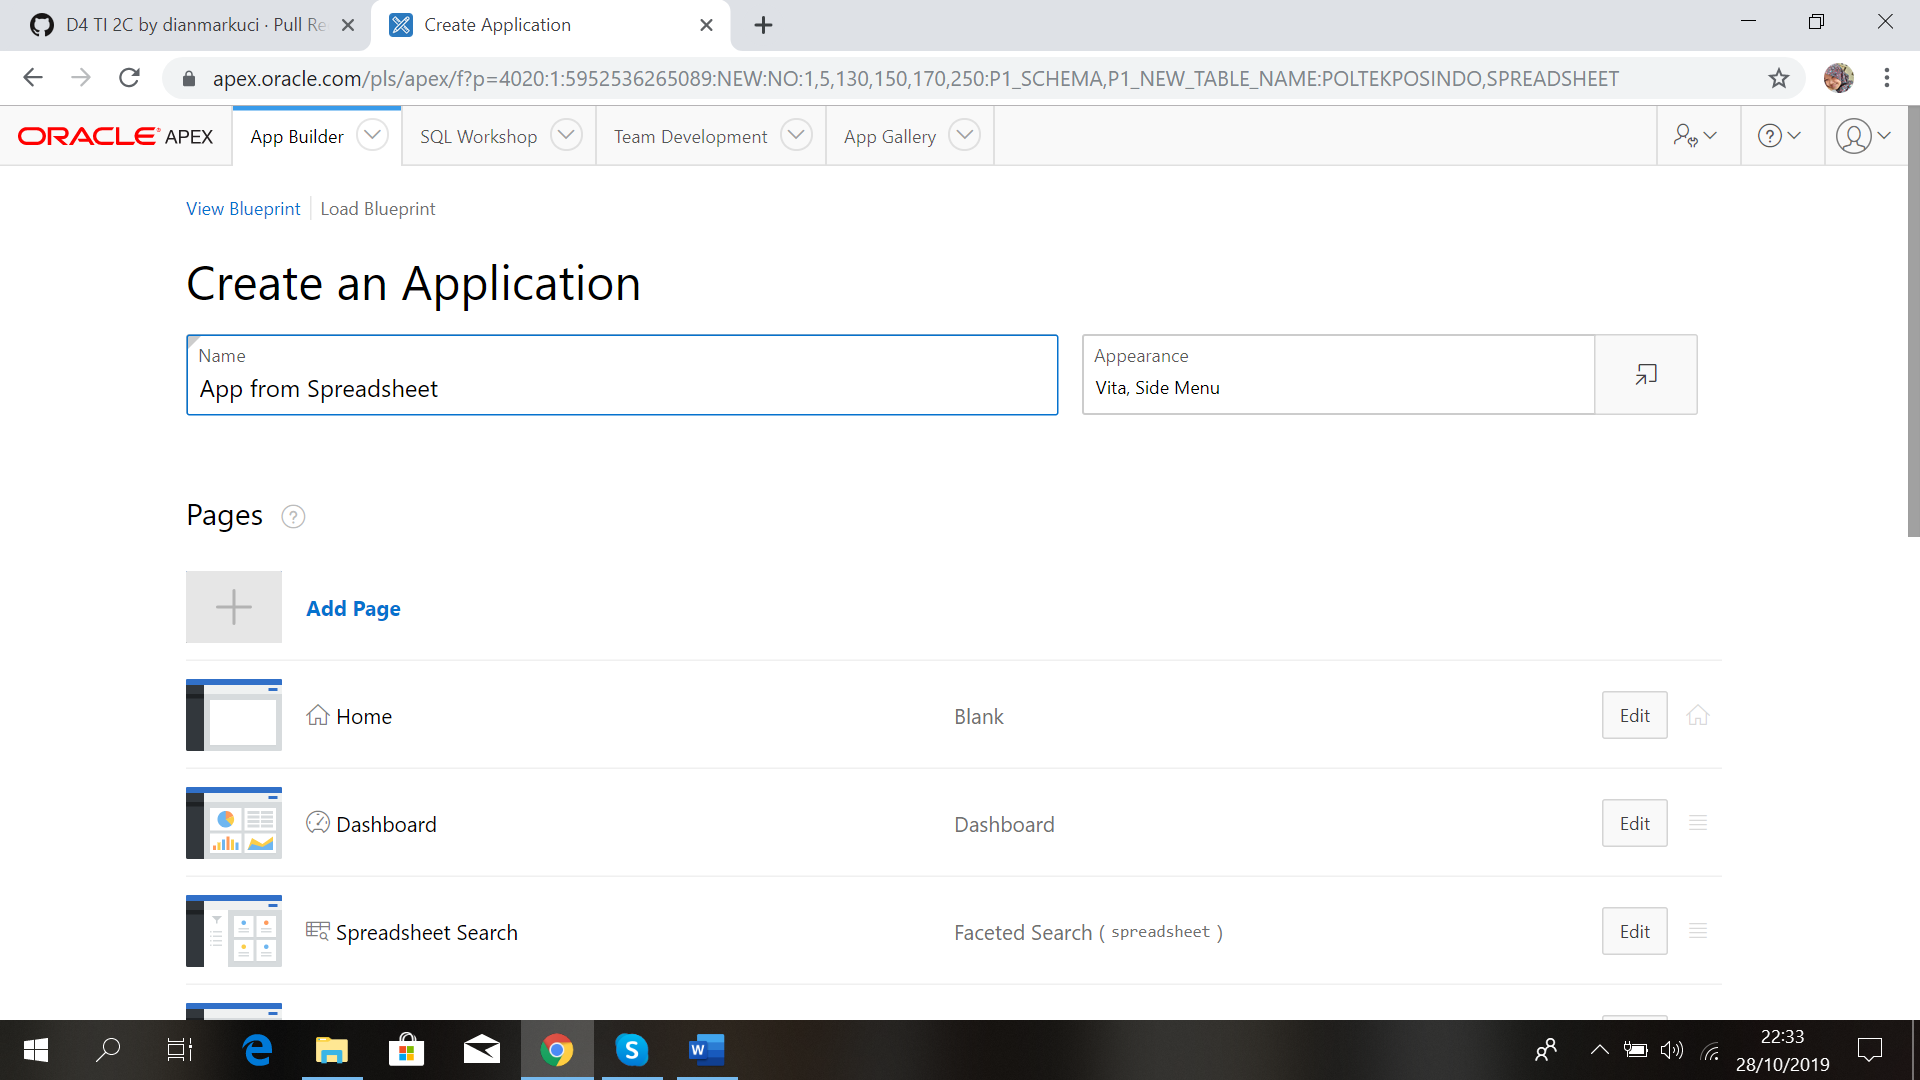
\includegraphics[width=10cm\textwidth]{figure/11.png}
  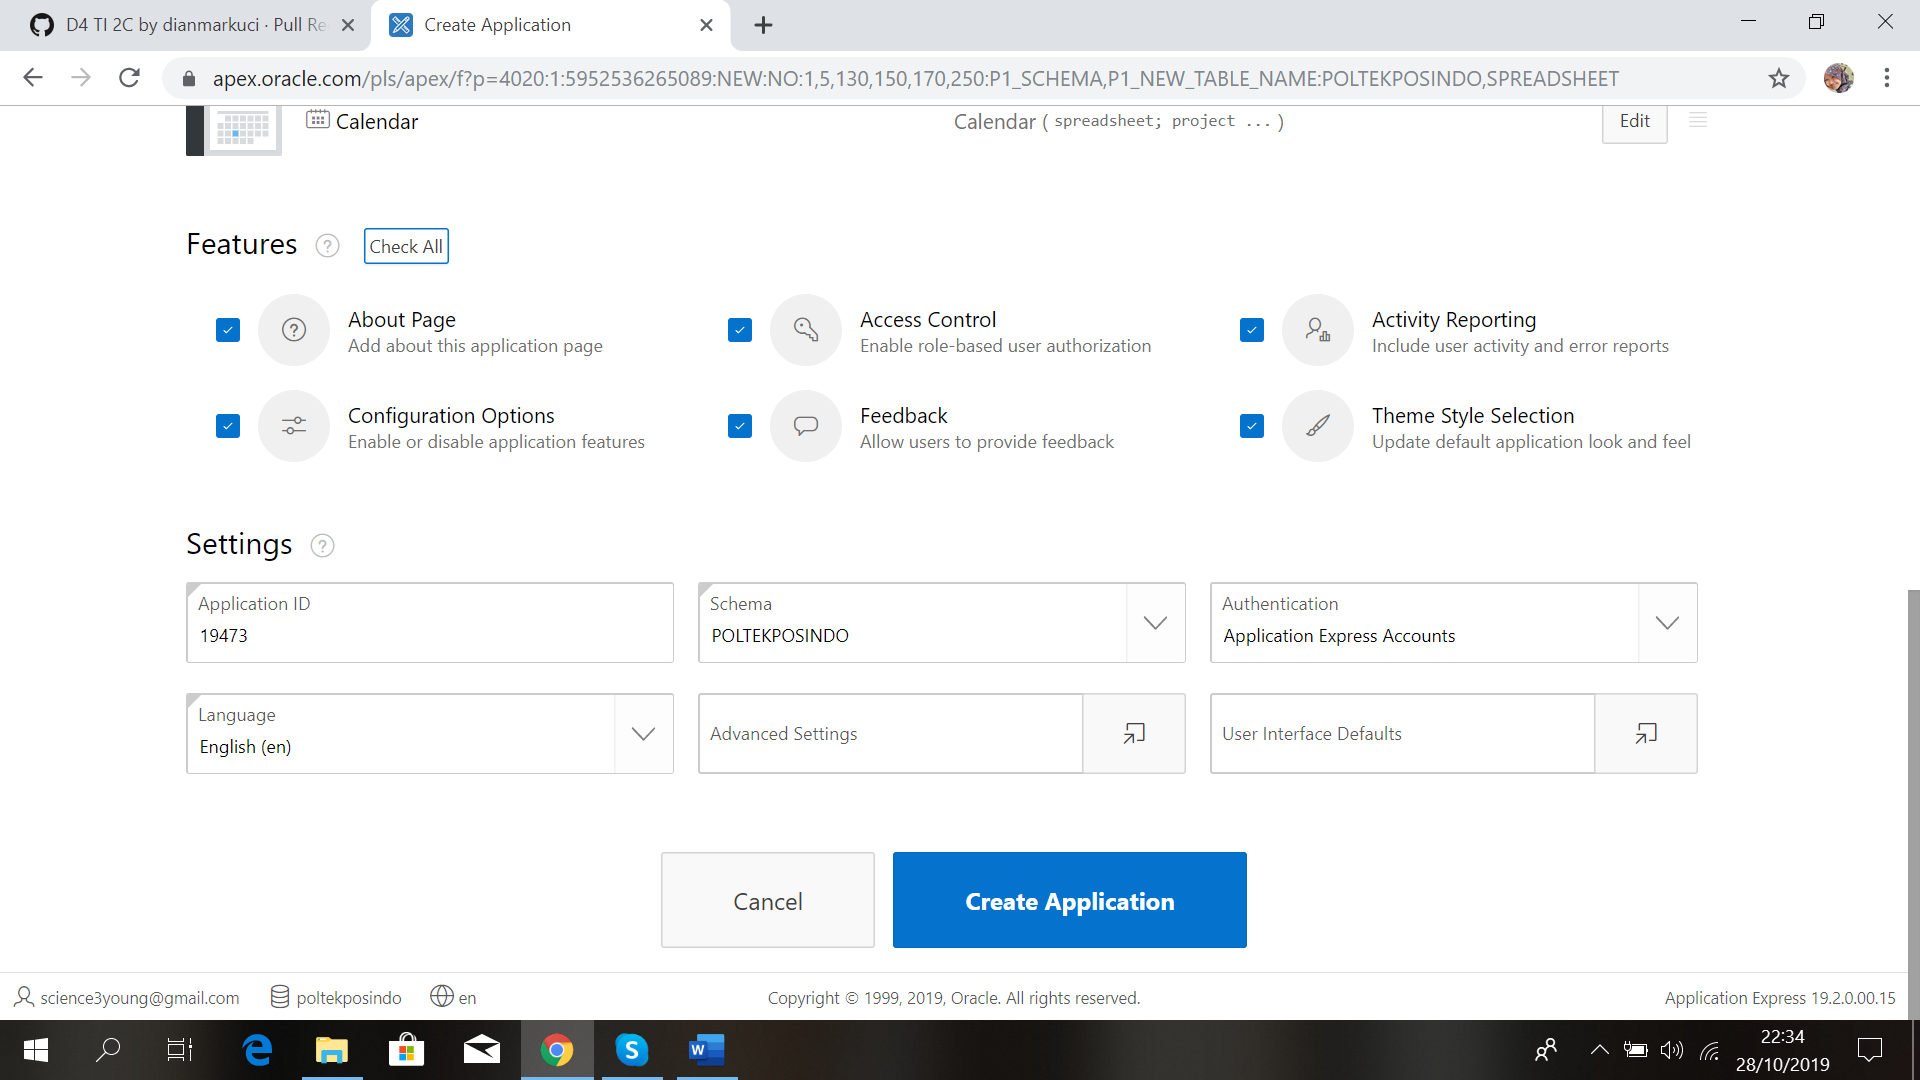
\includegraphics[width=10cm\textwidth]{figure/12.png}
\end{center}

\item 9. Sign In
\begin{center}
  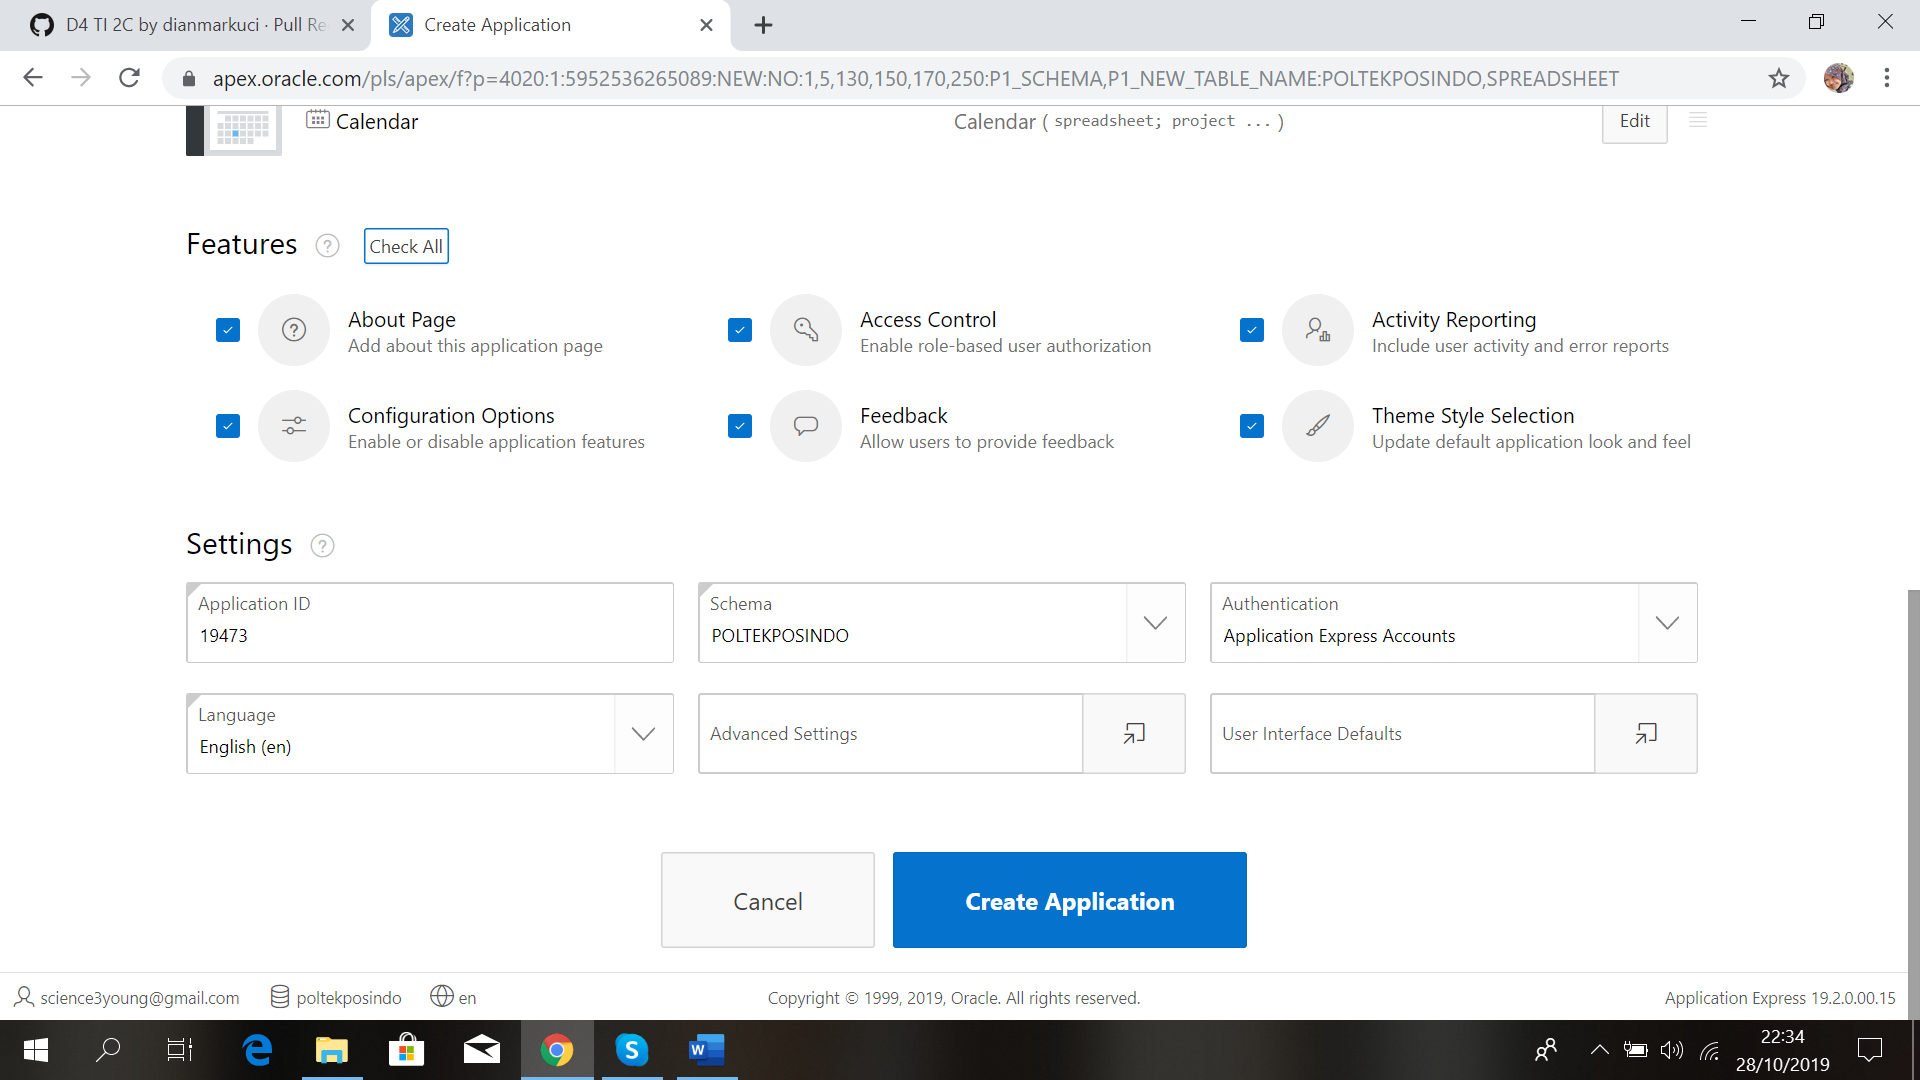
\includegraphics[width=10cm\textwidth]{figure/13.png}
  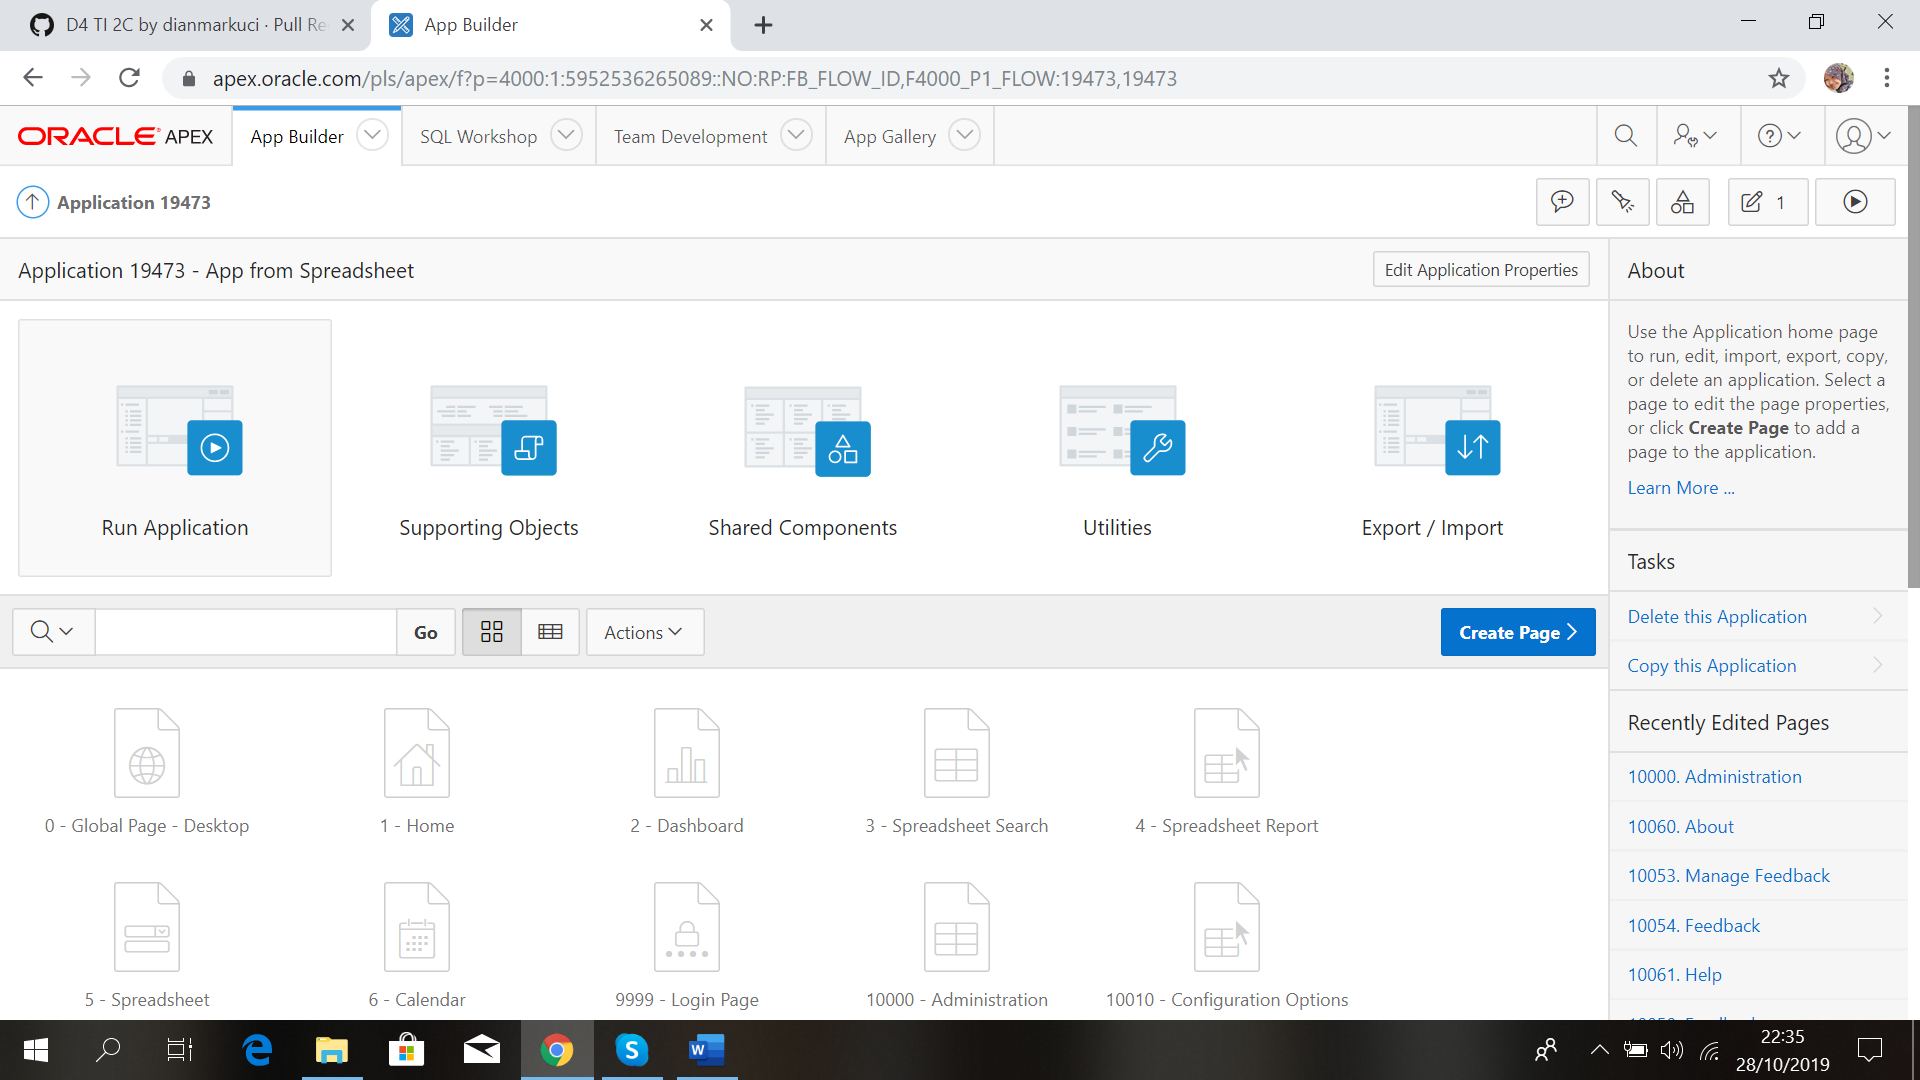
\includegraphics[width=10cm\textwidth]{figure/14.png}
  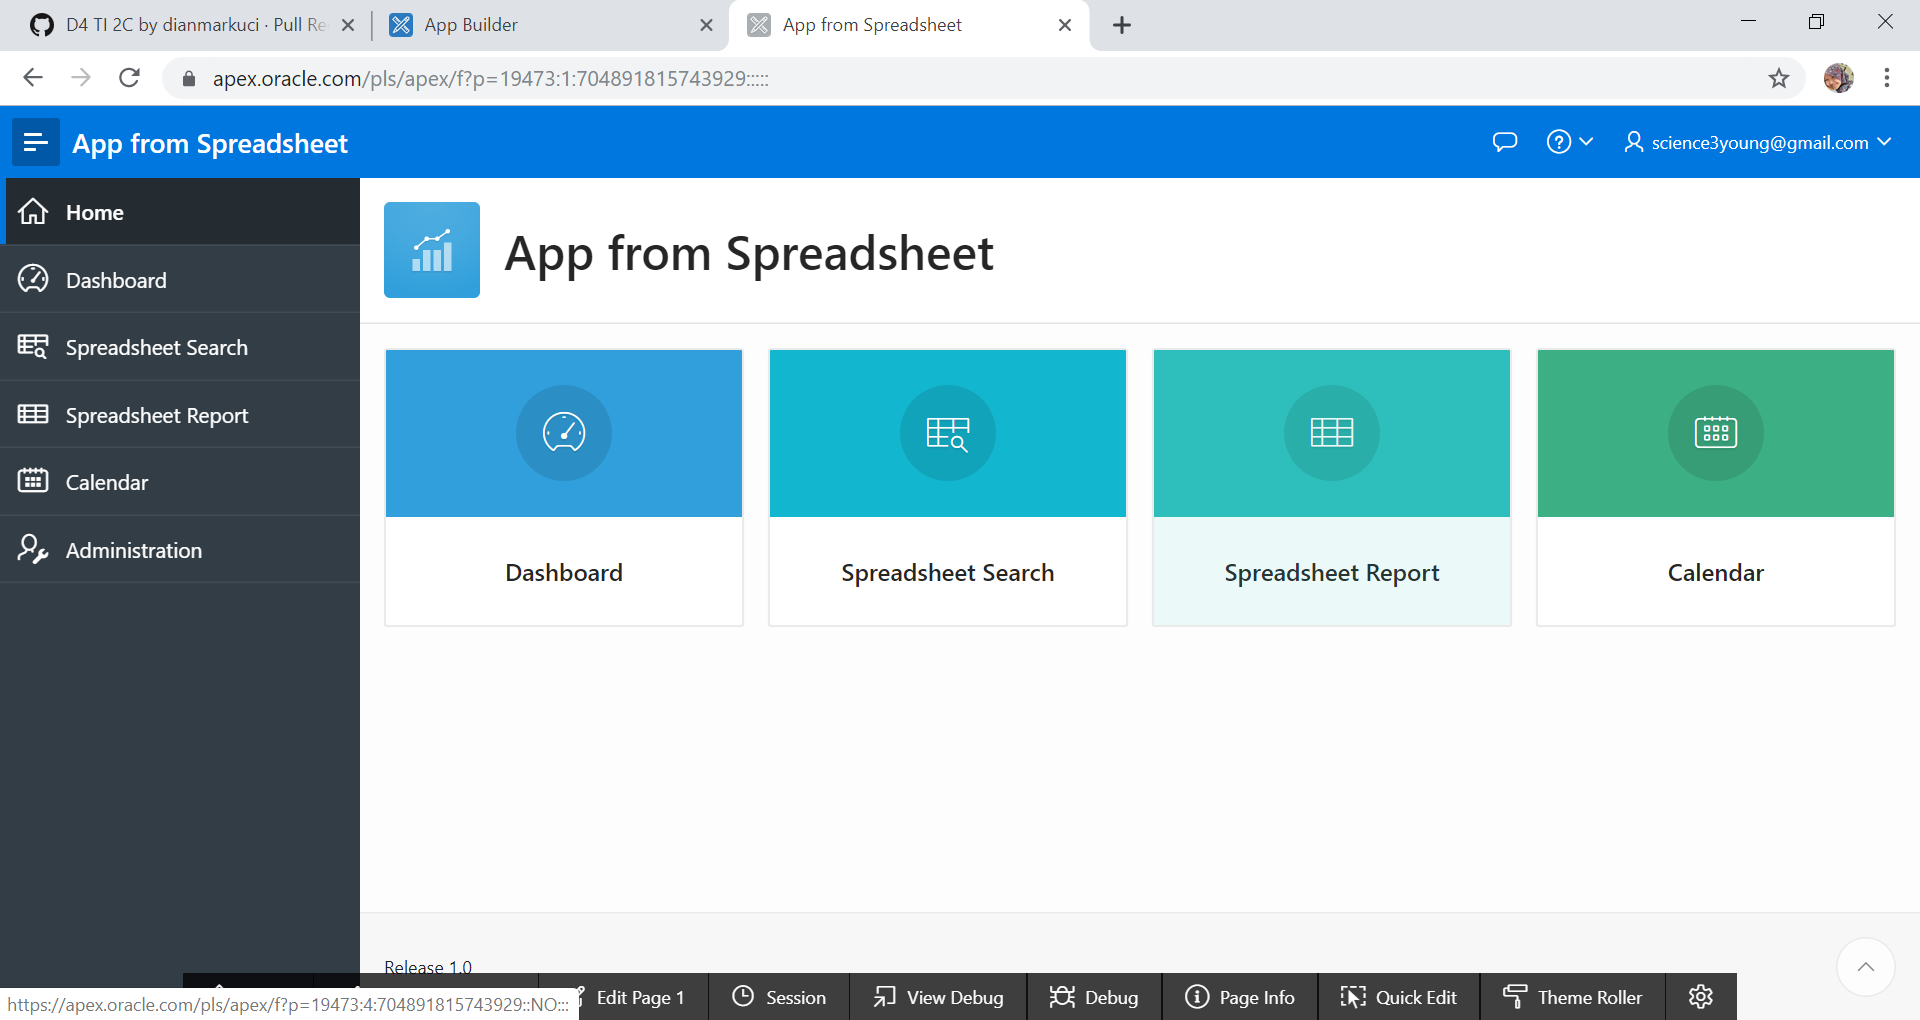
\includegraphics[width=10cm\textwidth]{figure/15.png}
\end{center}

\item 10. Mengurutkan Laporan
\begin{center}
  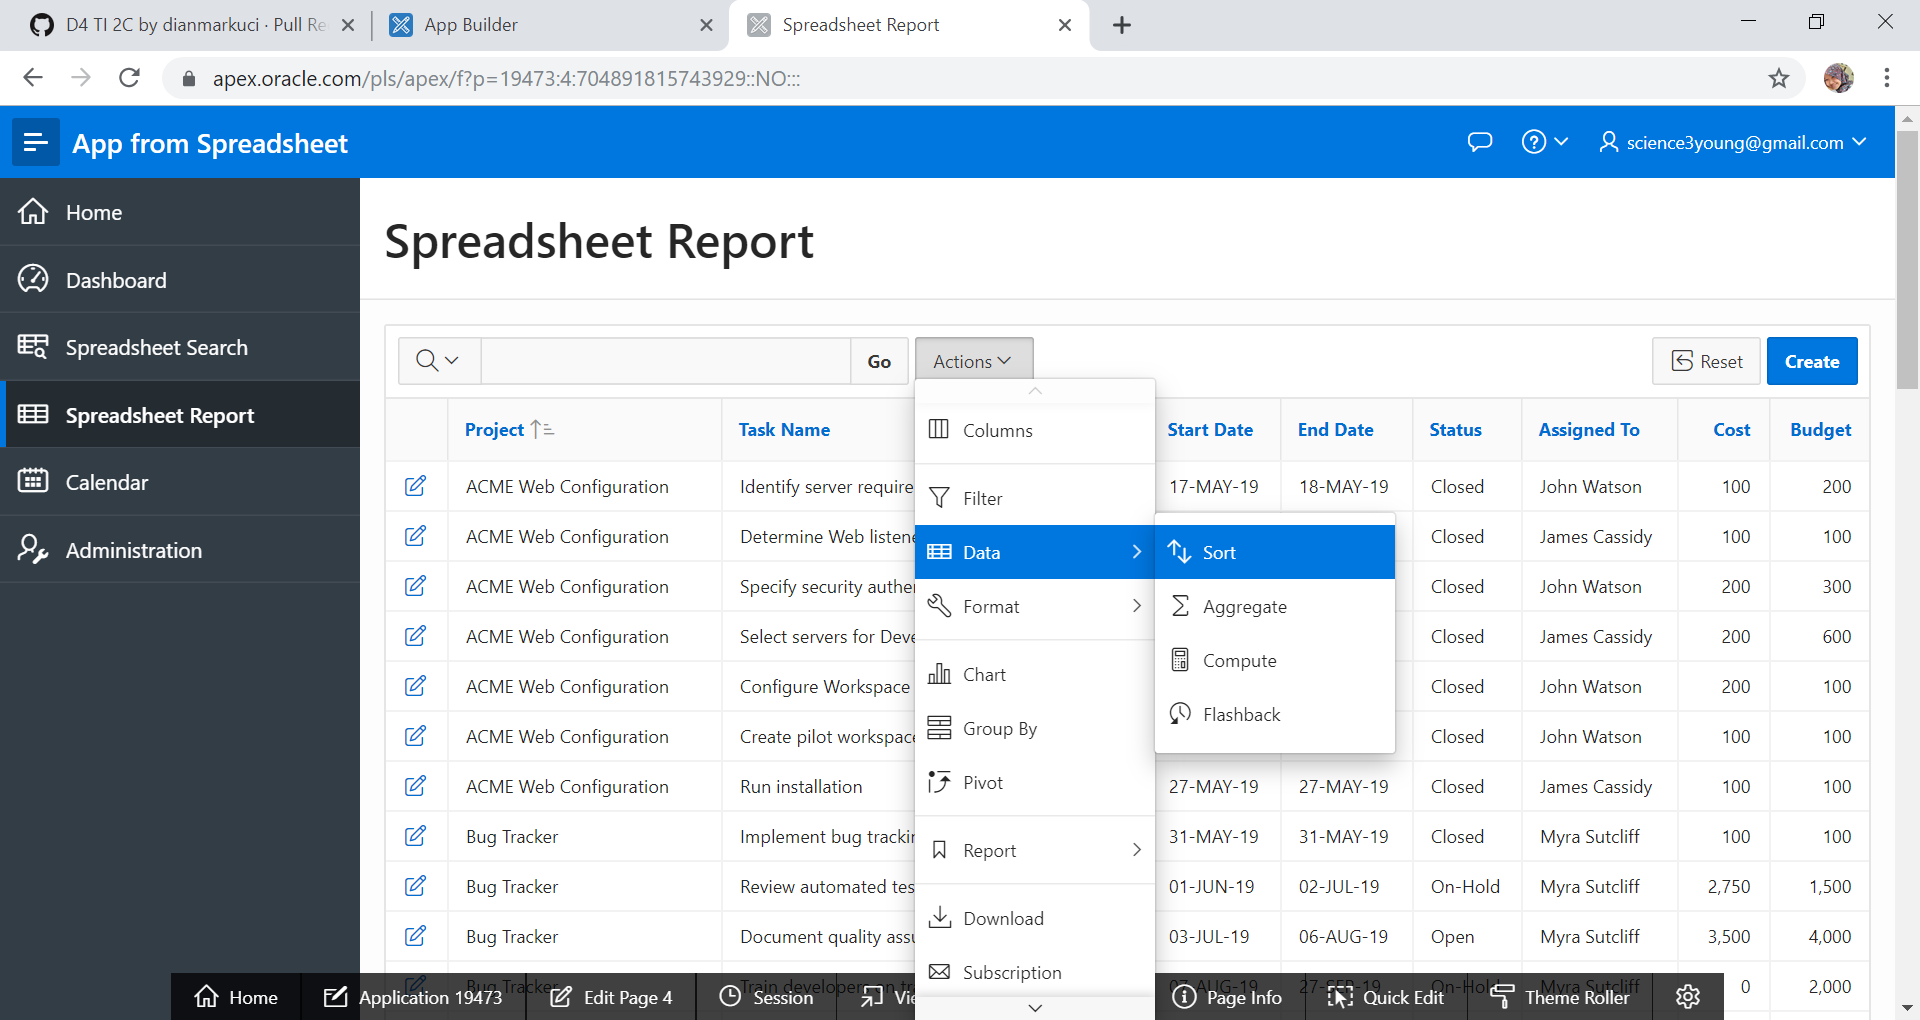
\includegraphics[width=10cm\textwidth]{figure/16.png}
  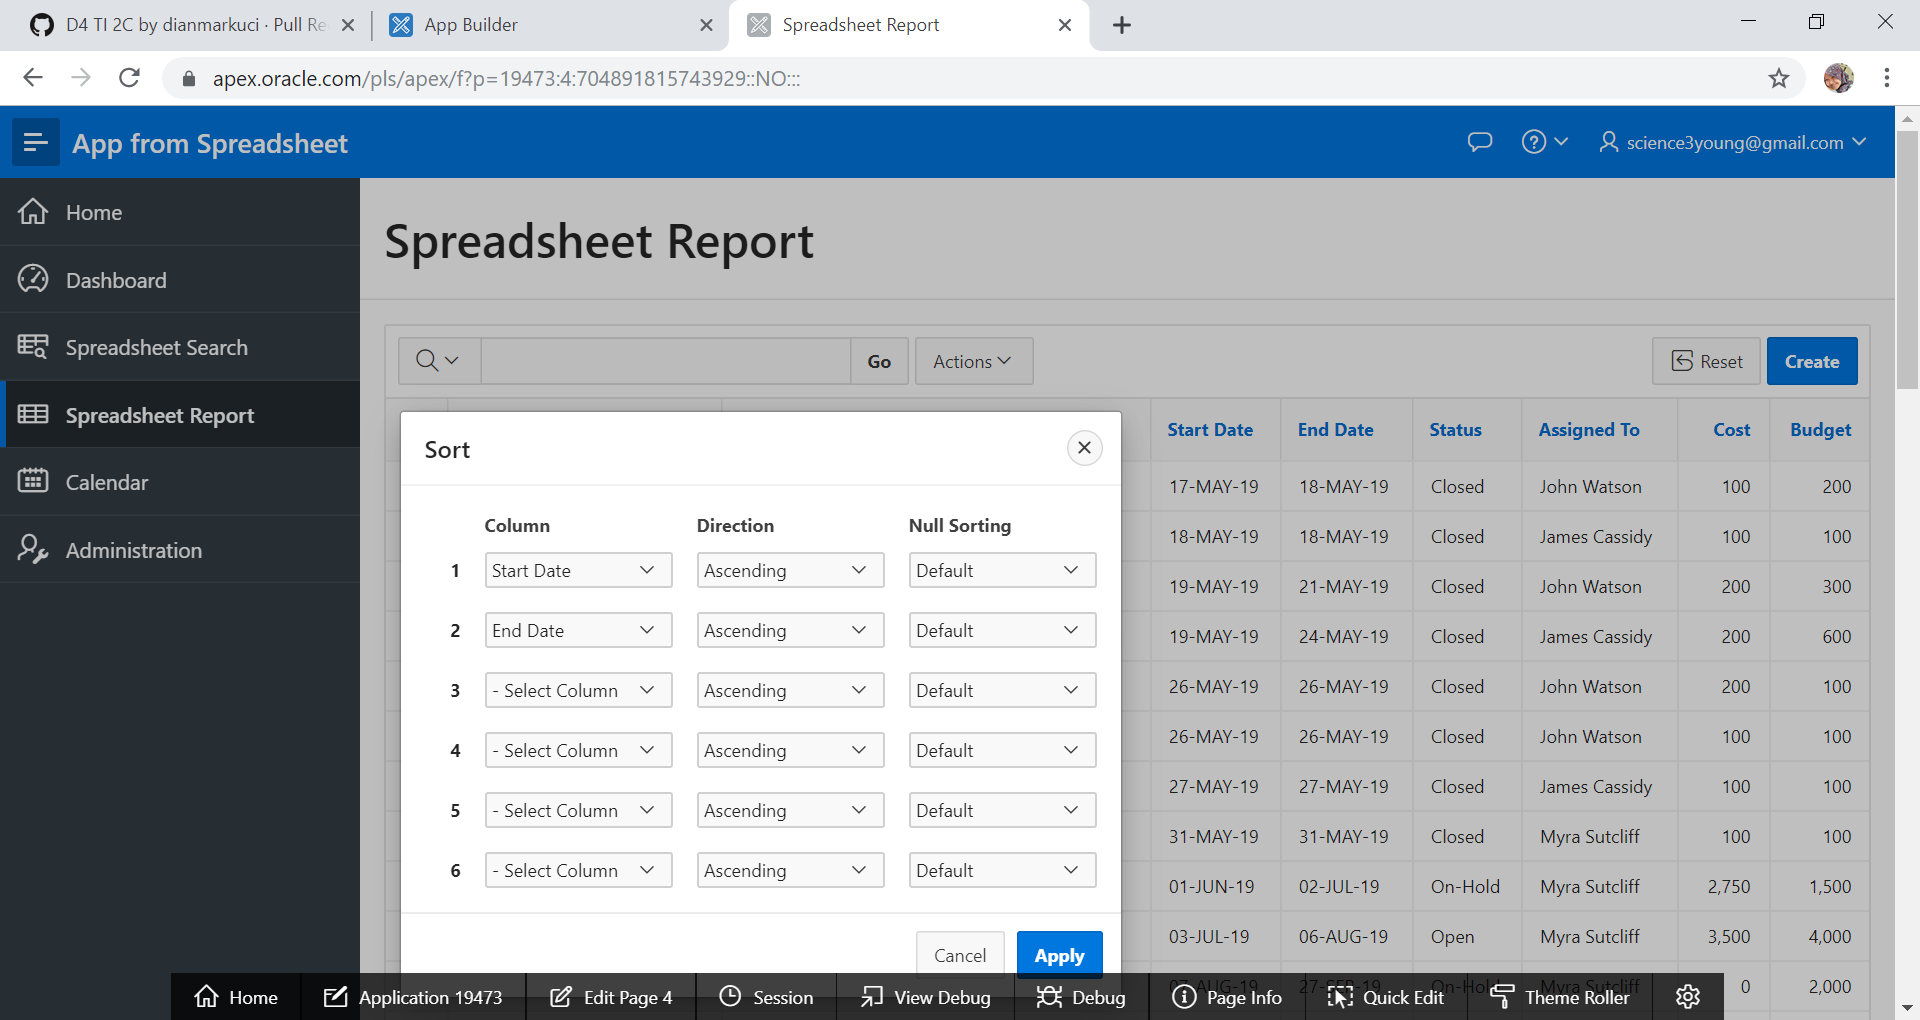
\includegraphics[width=10cm\textwidth]{figure/17.png}
  
\end{center}

\item 11. Menambah Komputasi
\begin{center}
    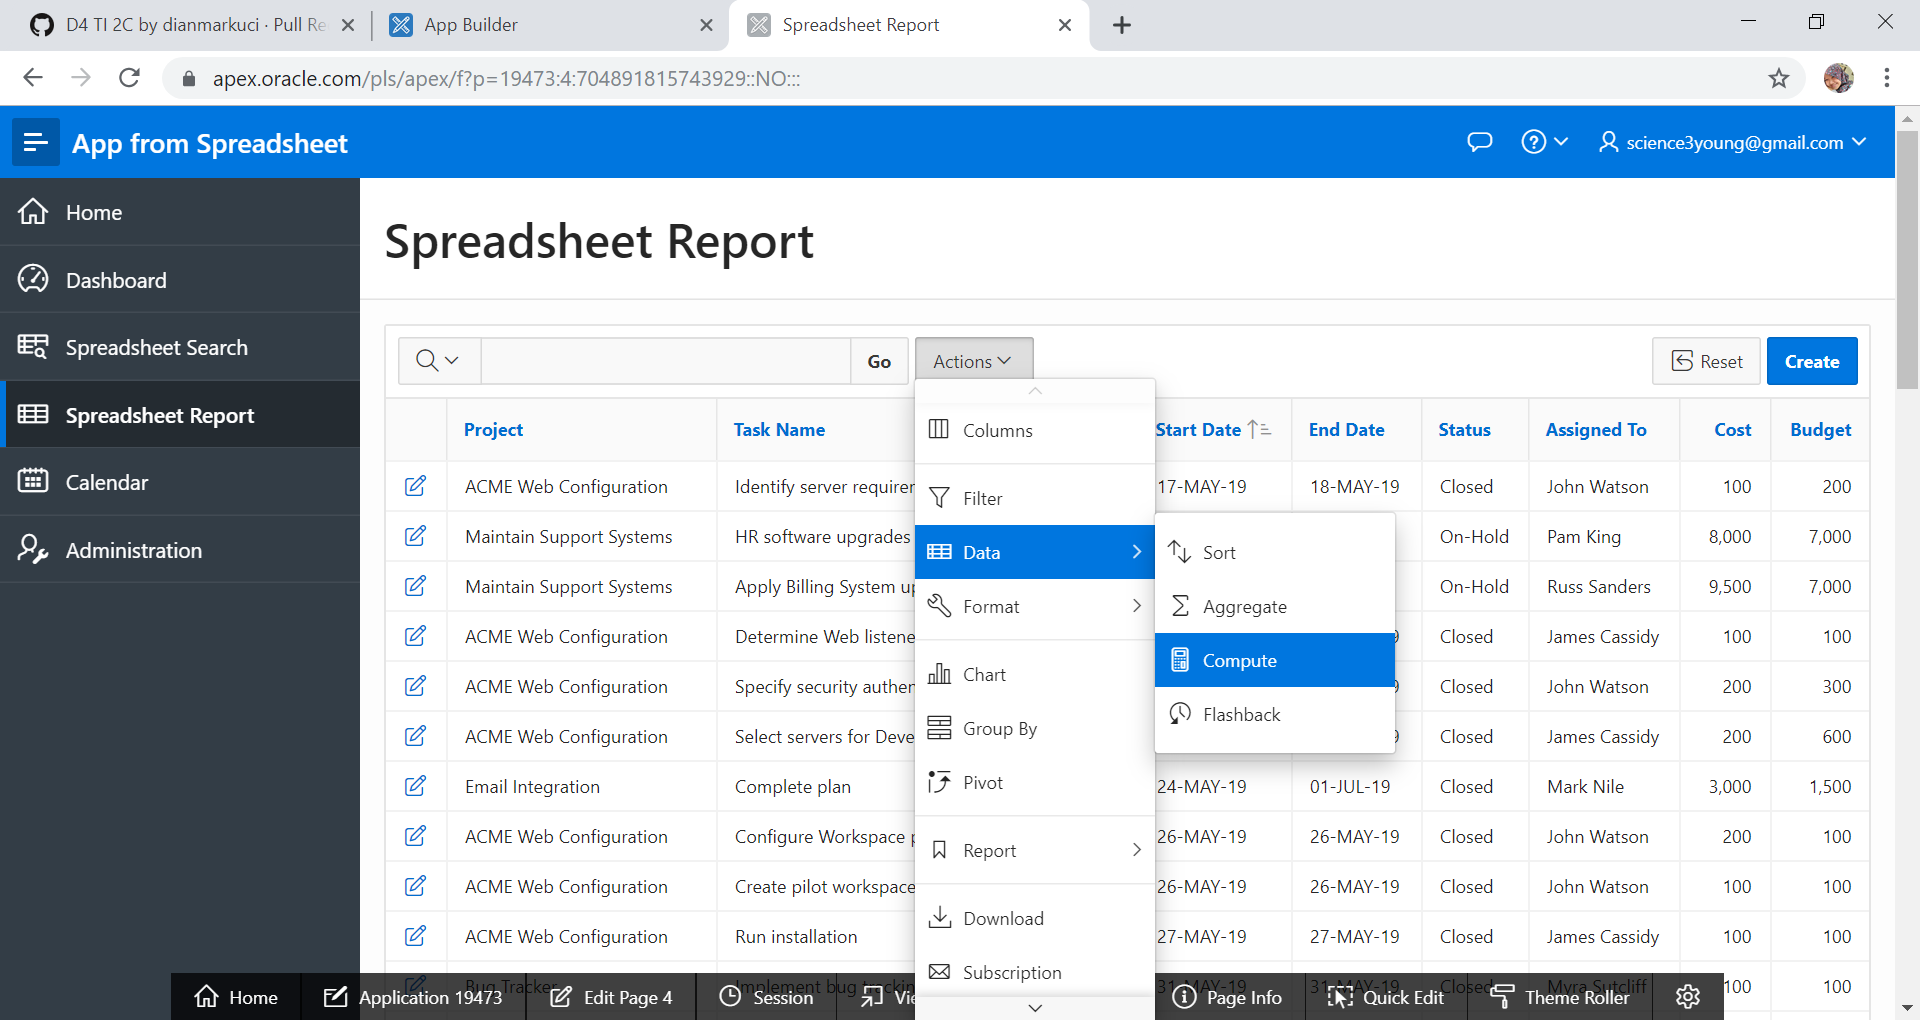
\includegraphics[width=10cm\textwidth]{figure/18.png}
    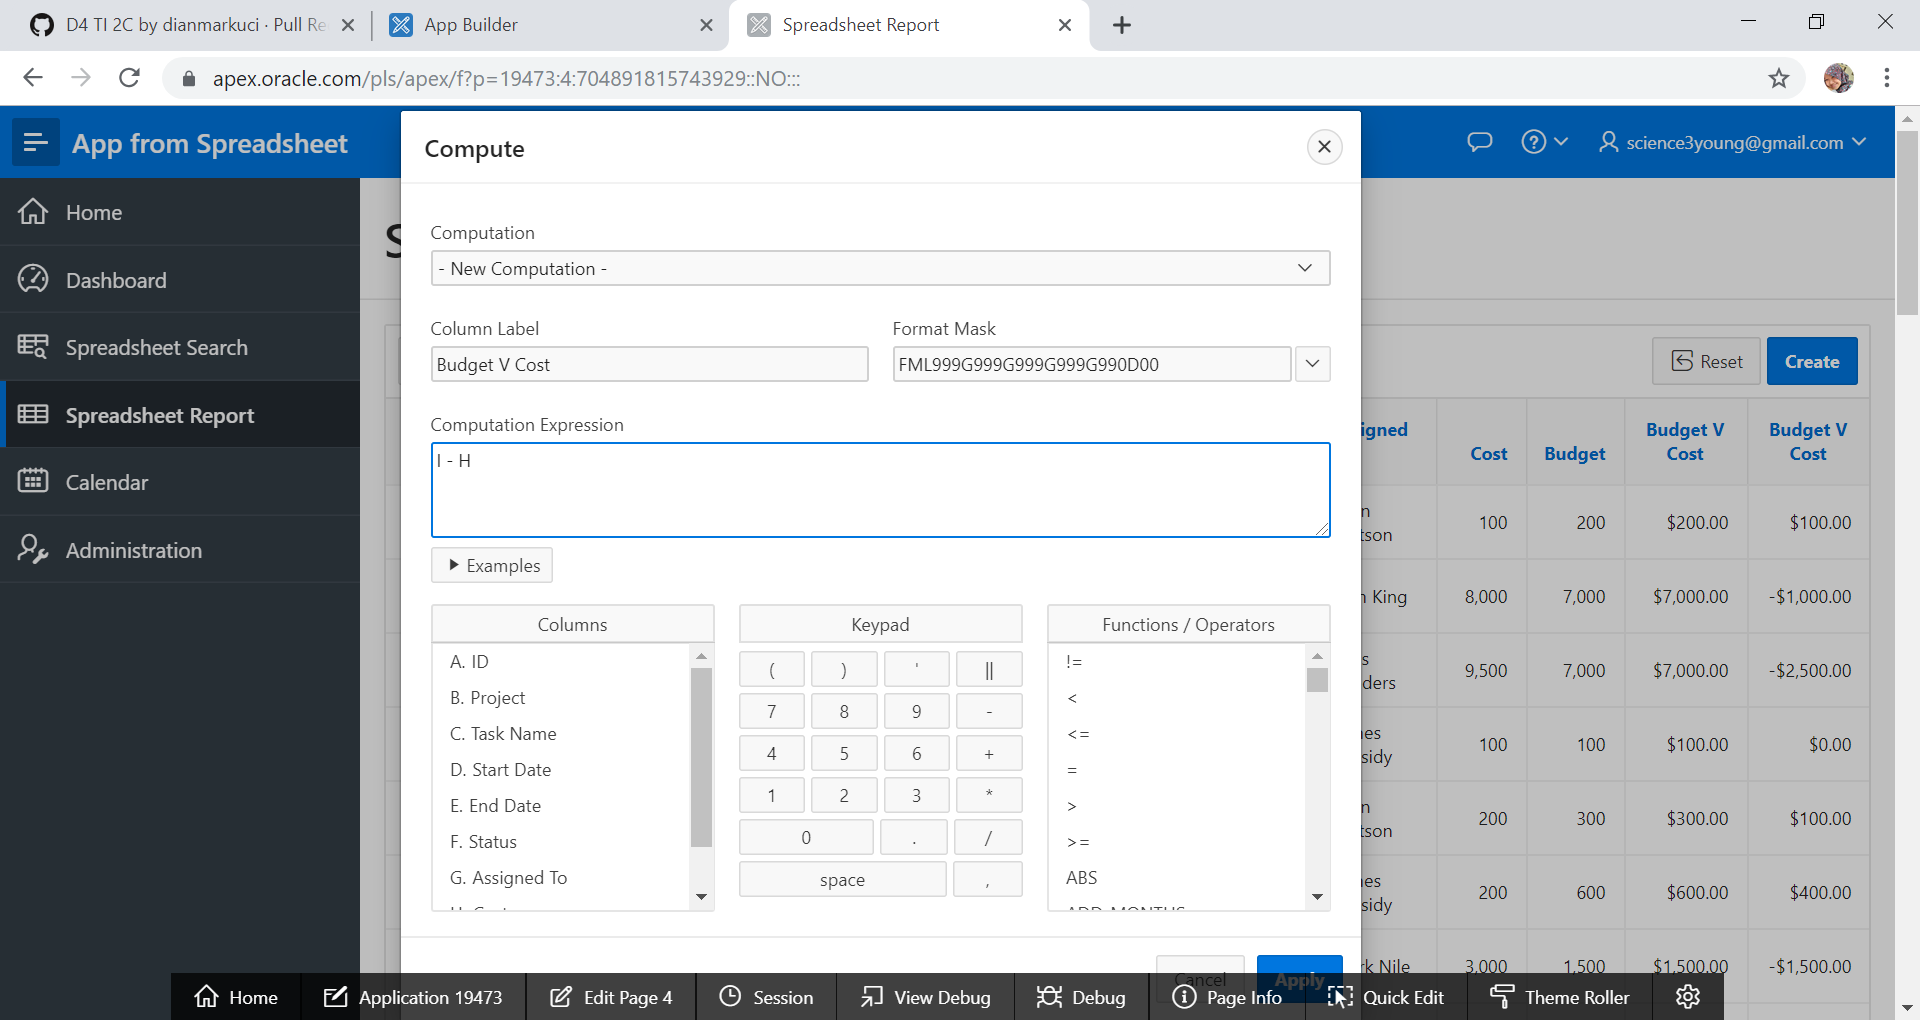
\includegraphics[width=10cm\textwidth]{figure/19.png}
    
\end{center}

\item 12. Menyimpan File
\begin{center}
    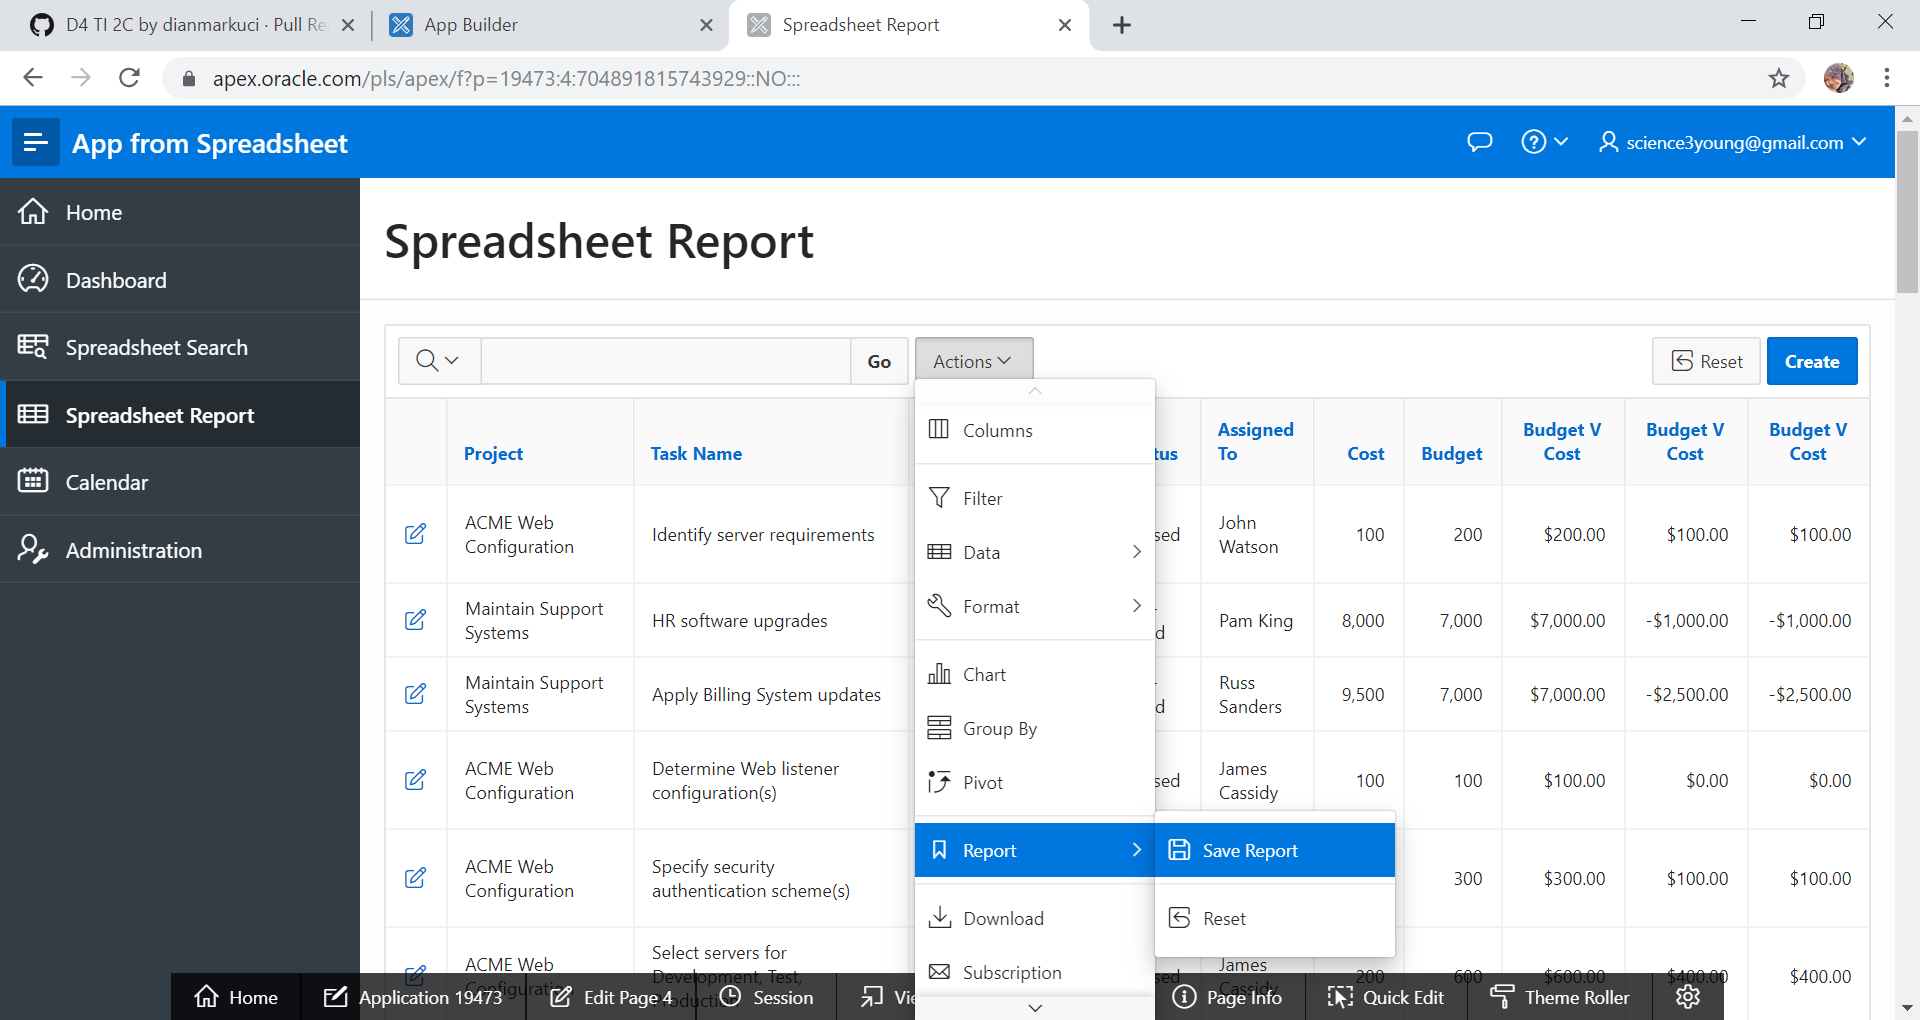
\includegraphics[width=10cm\textwidth]{figure/20.png}
    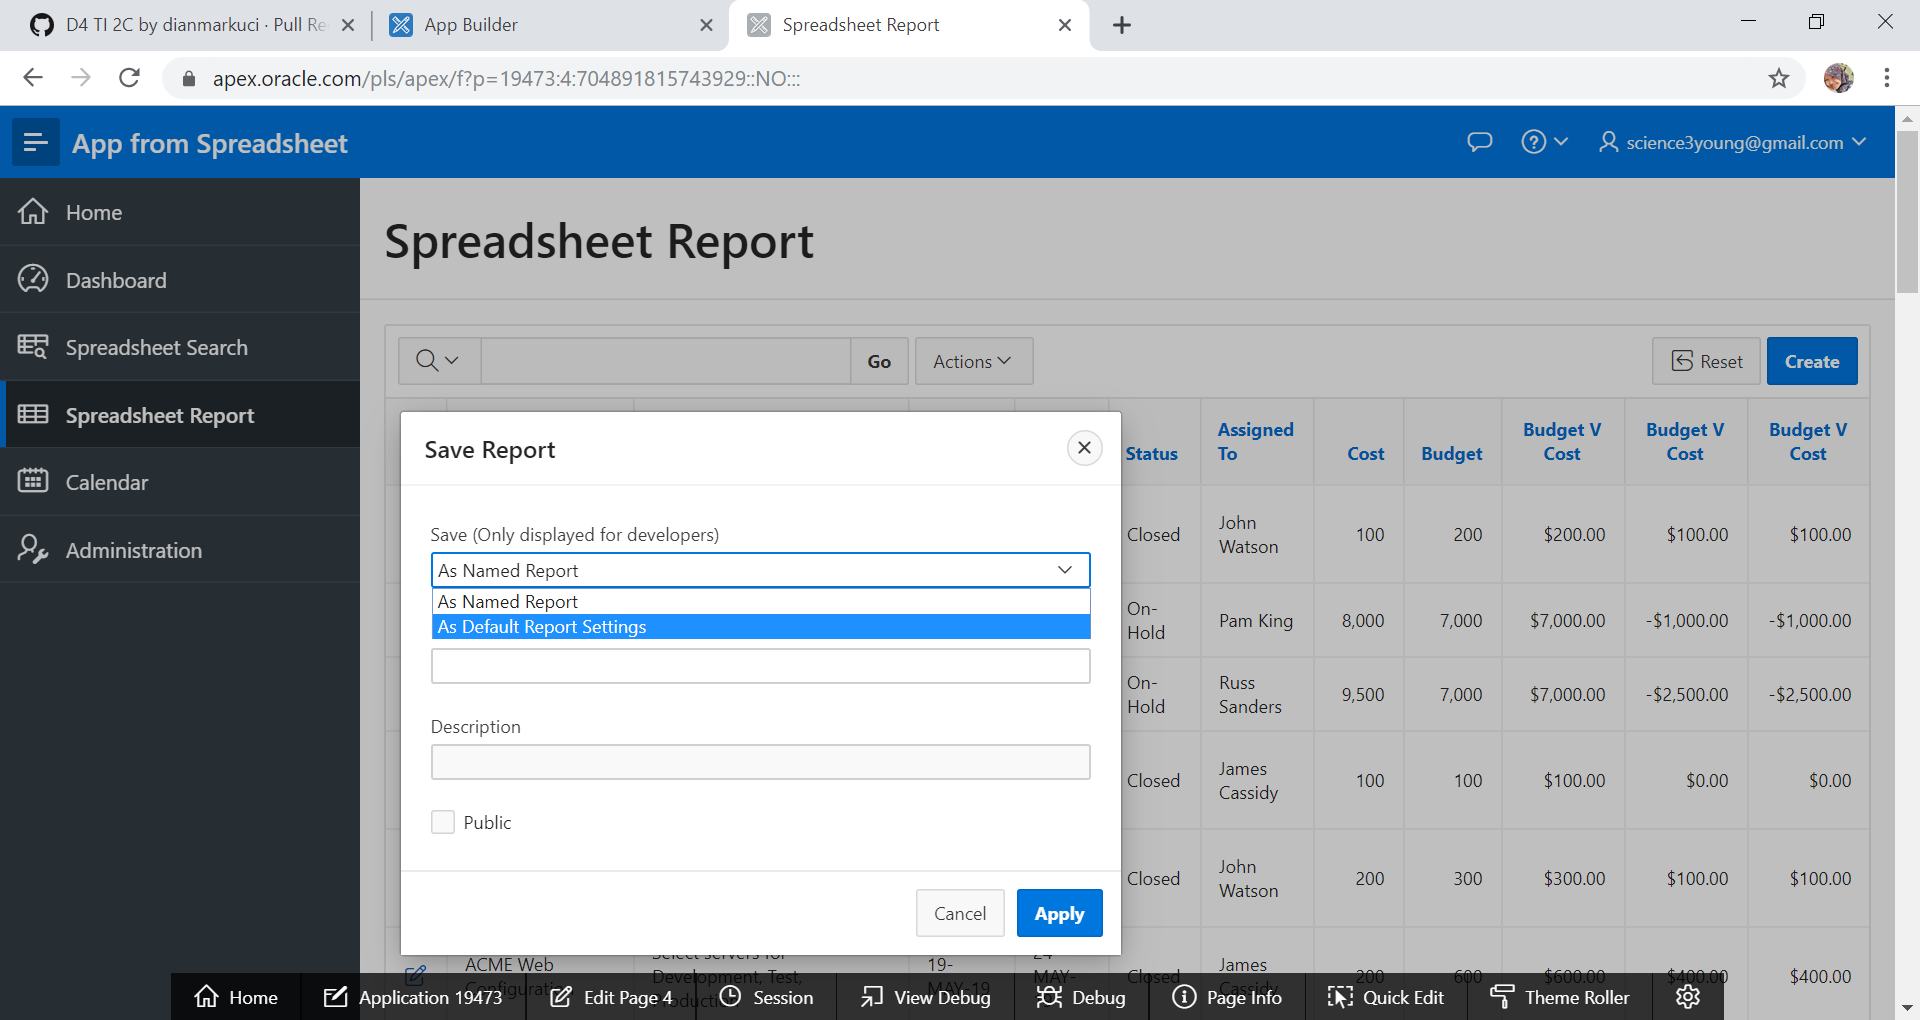
\includegraphics[width=10cm\textwidth]{figure/21.png}
    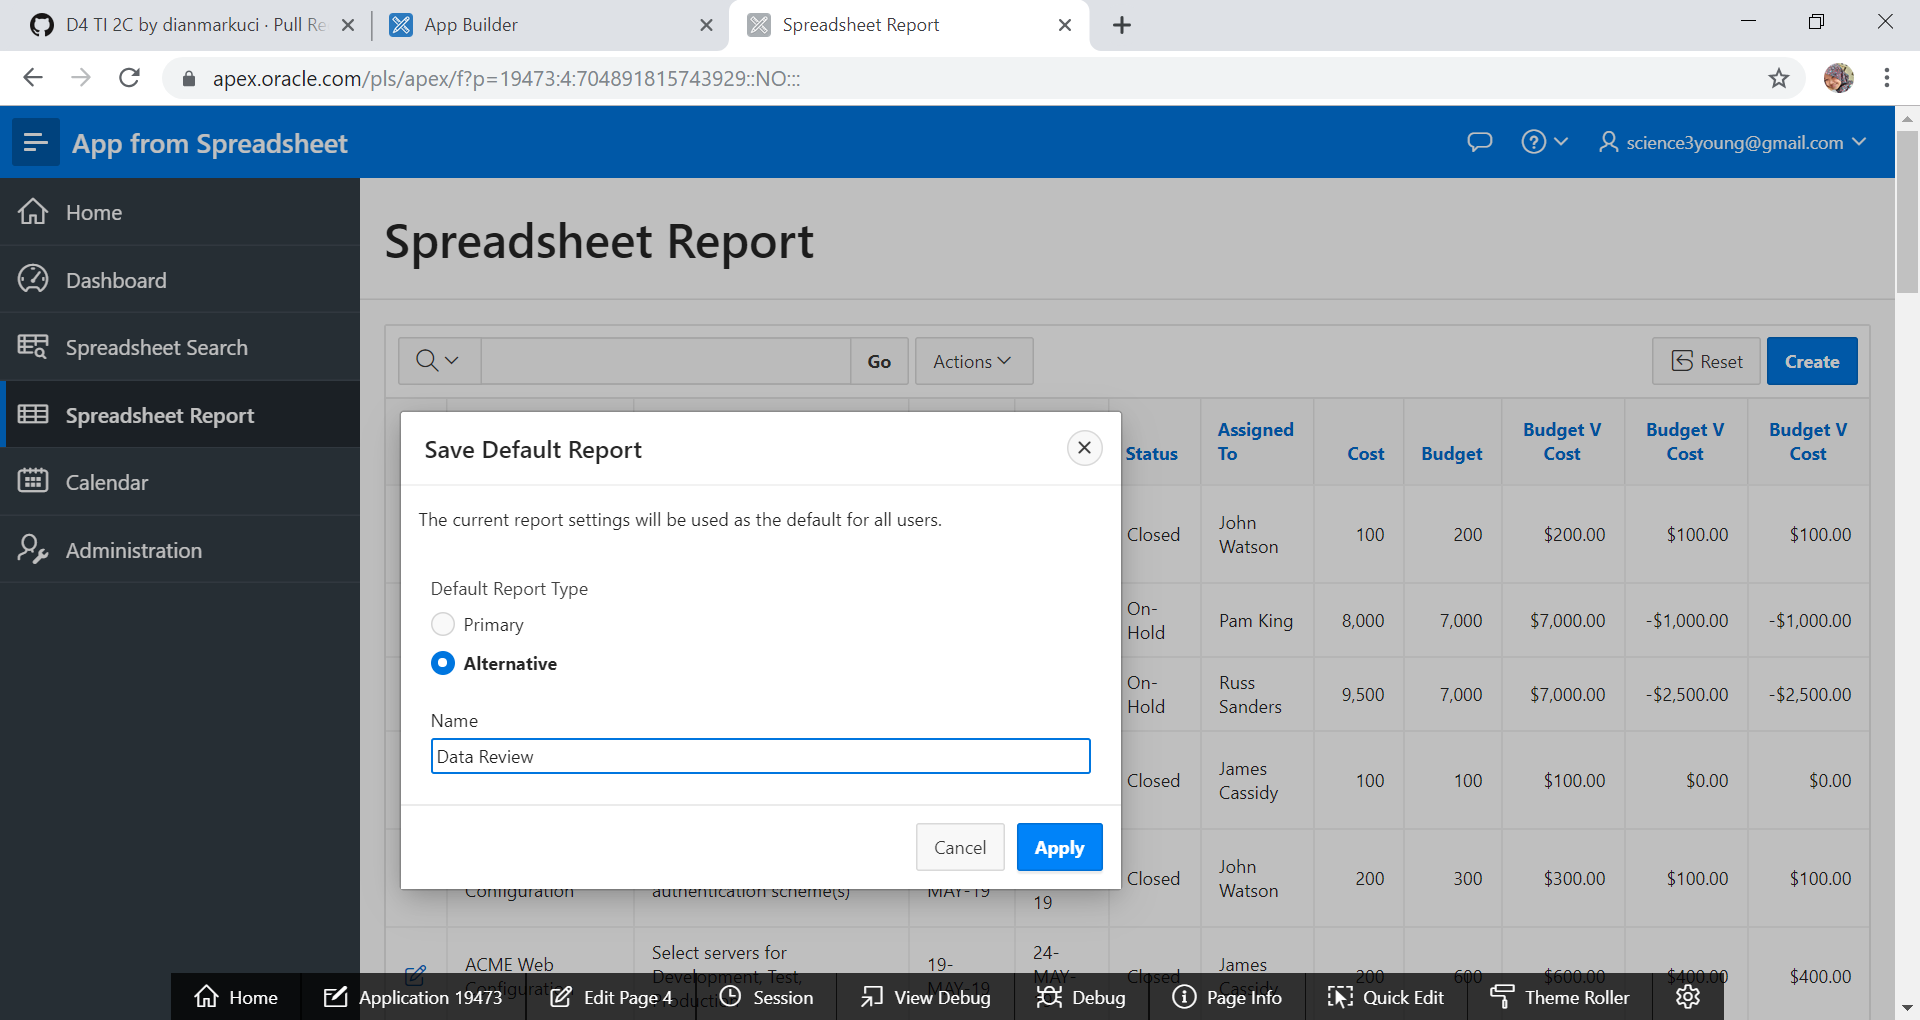
\includegraphics[width=10cm\textwidth]{figure/22.png}
\end{center}

\item 13. Menambah Grafik
\begin{center}
    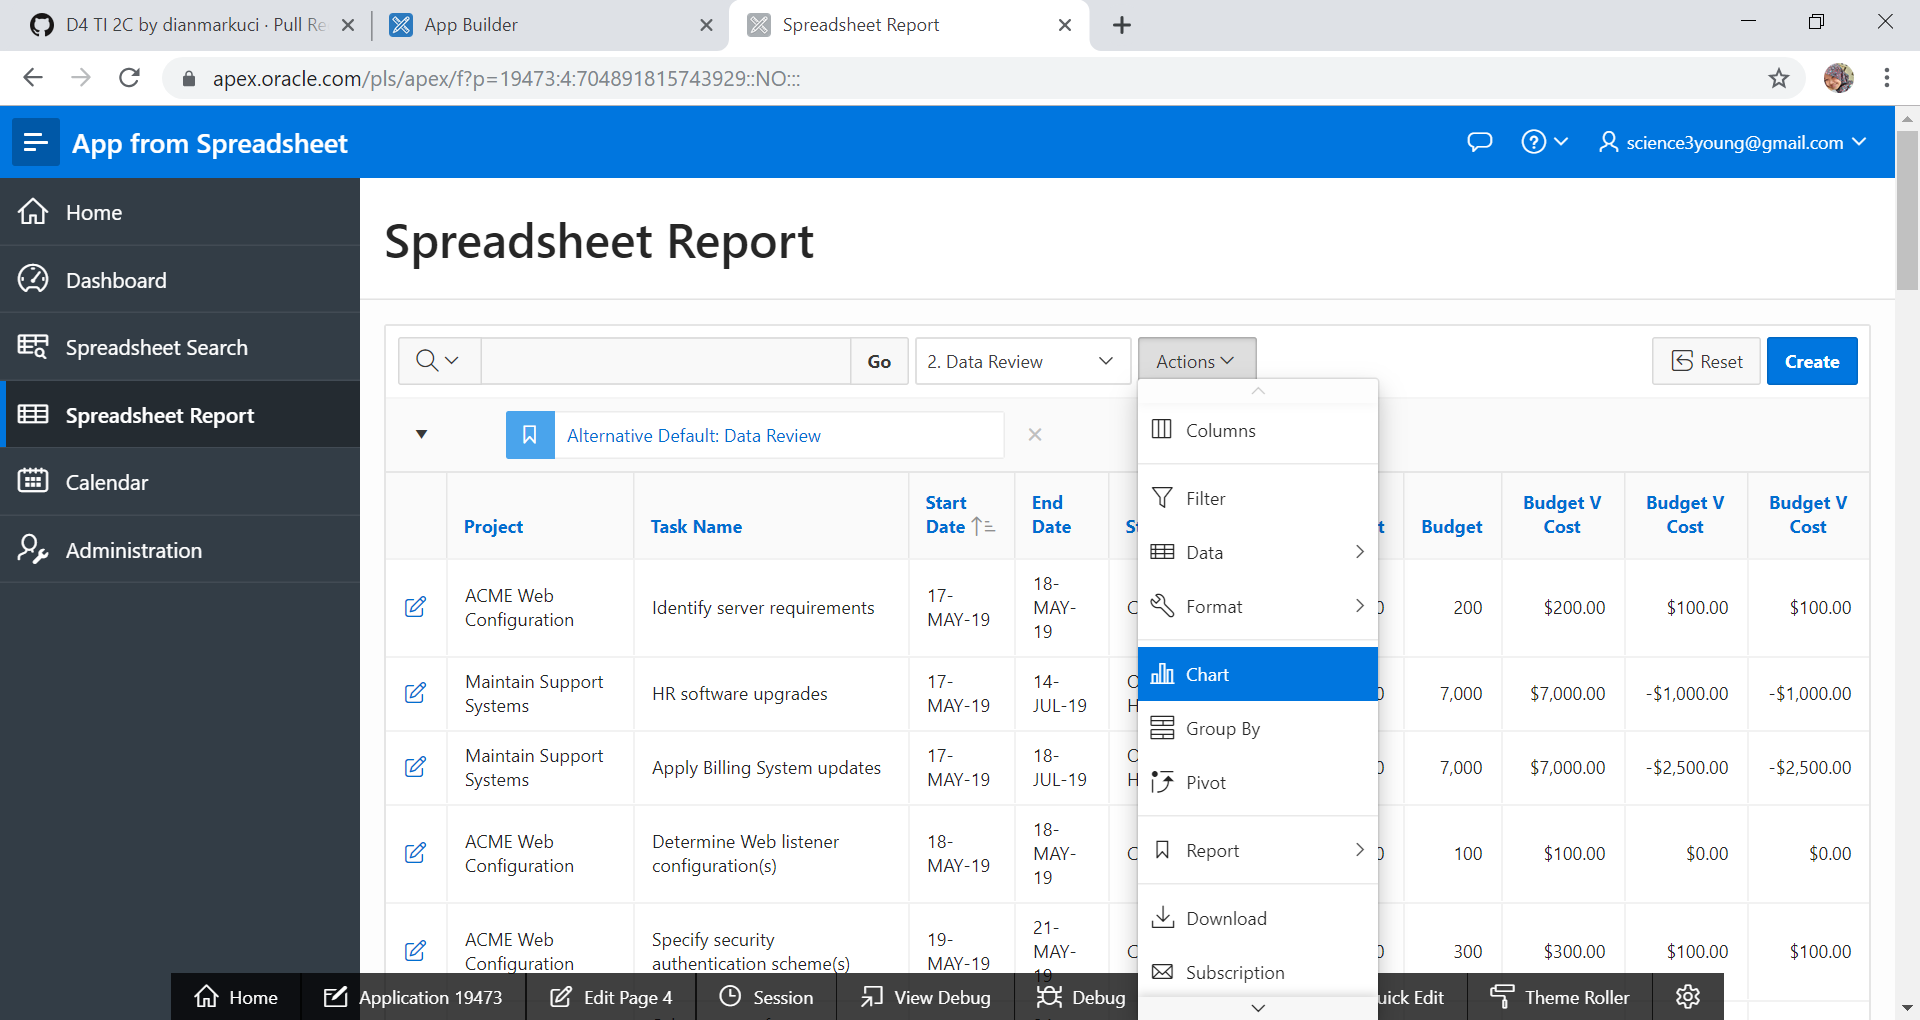
\includegraphics[width=10cm\textwidth]{figure/23.png}
    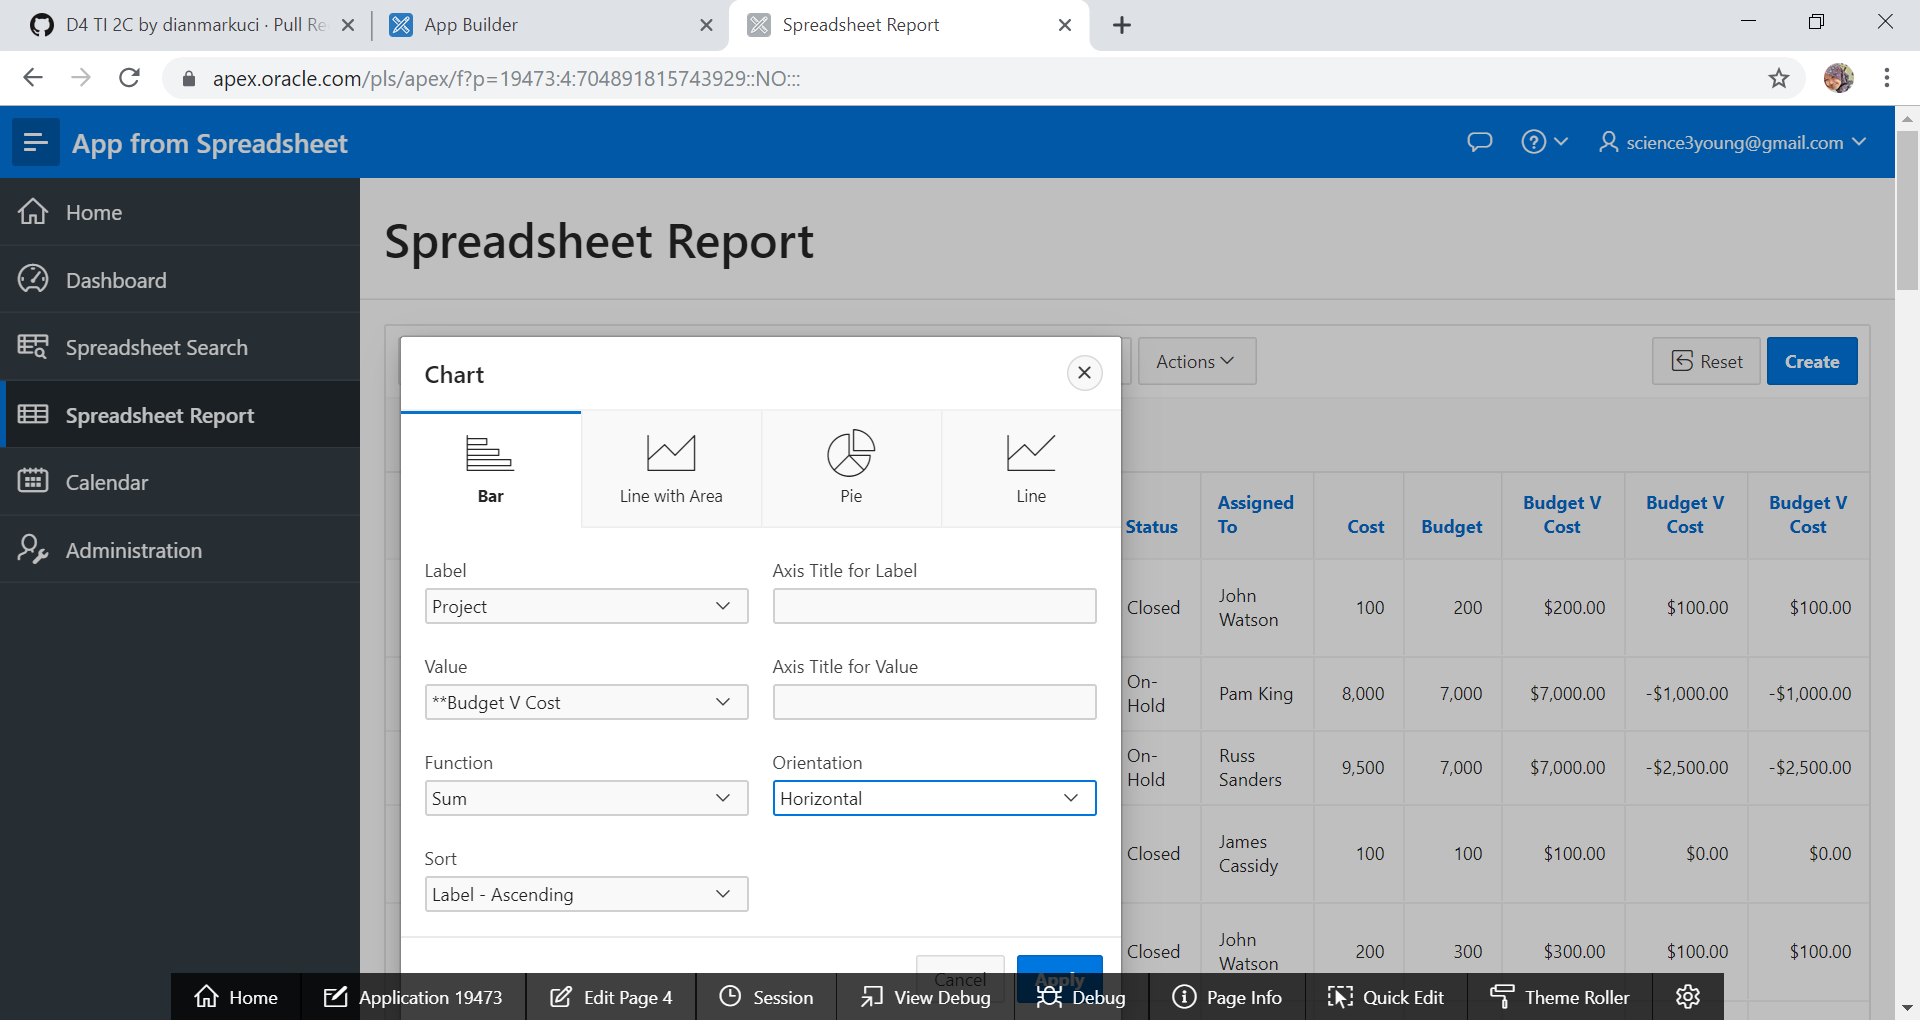
\includegraphics[width=10cm\textwidth]{figure/24.png}
    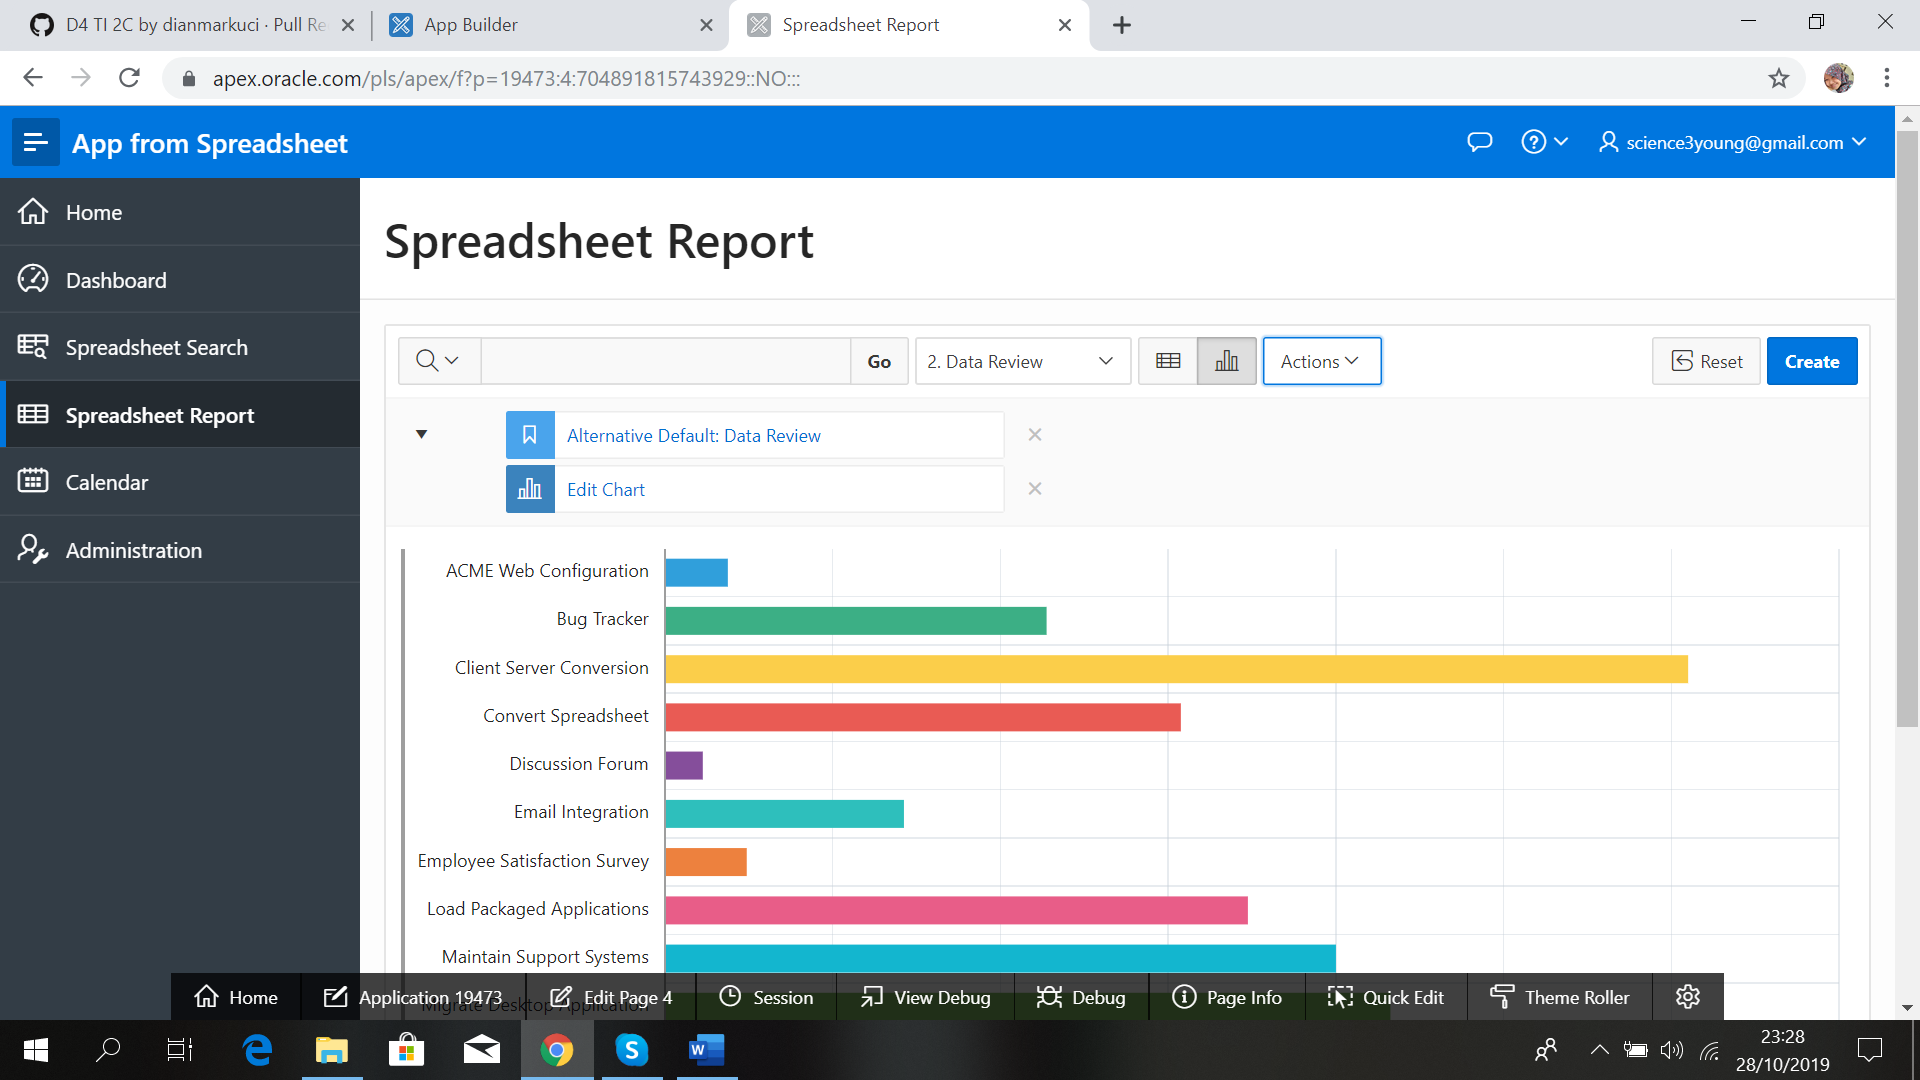
\includegraphics[width=10cm\textwidth]{figure/25.png}
    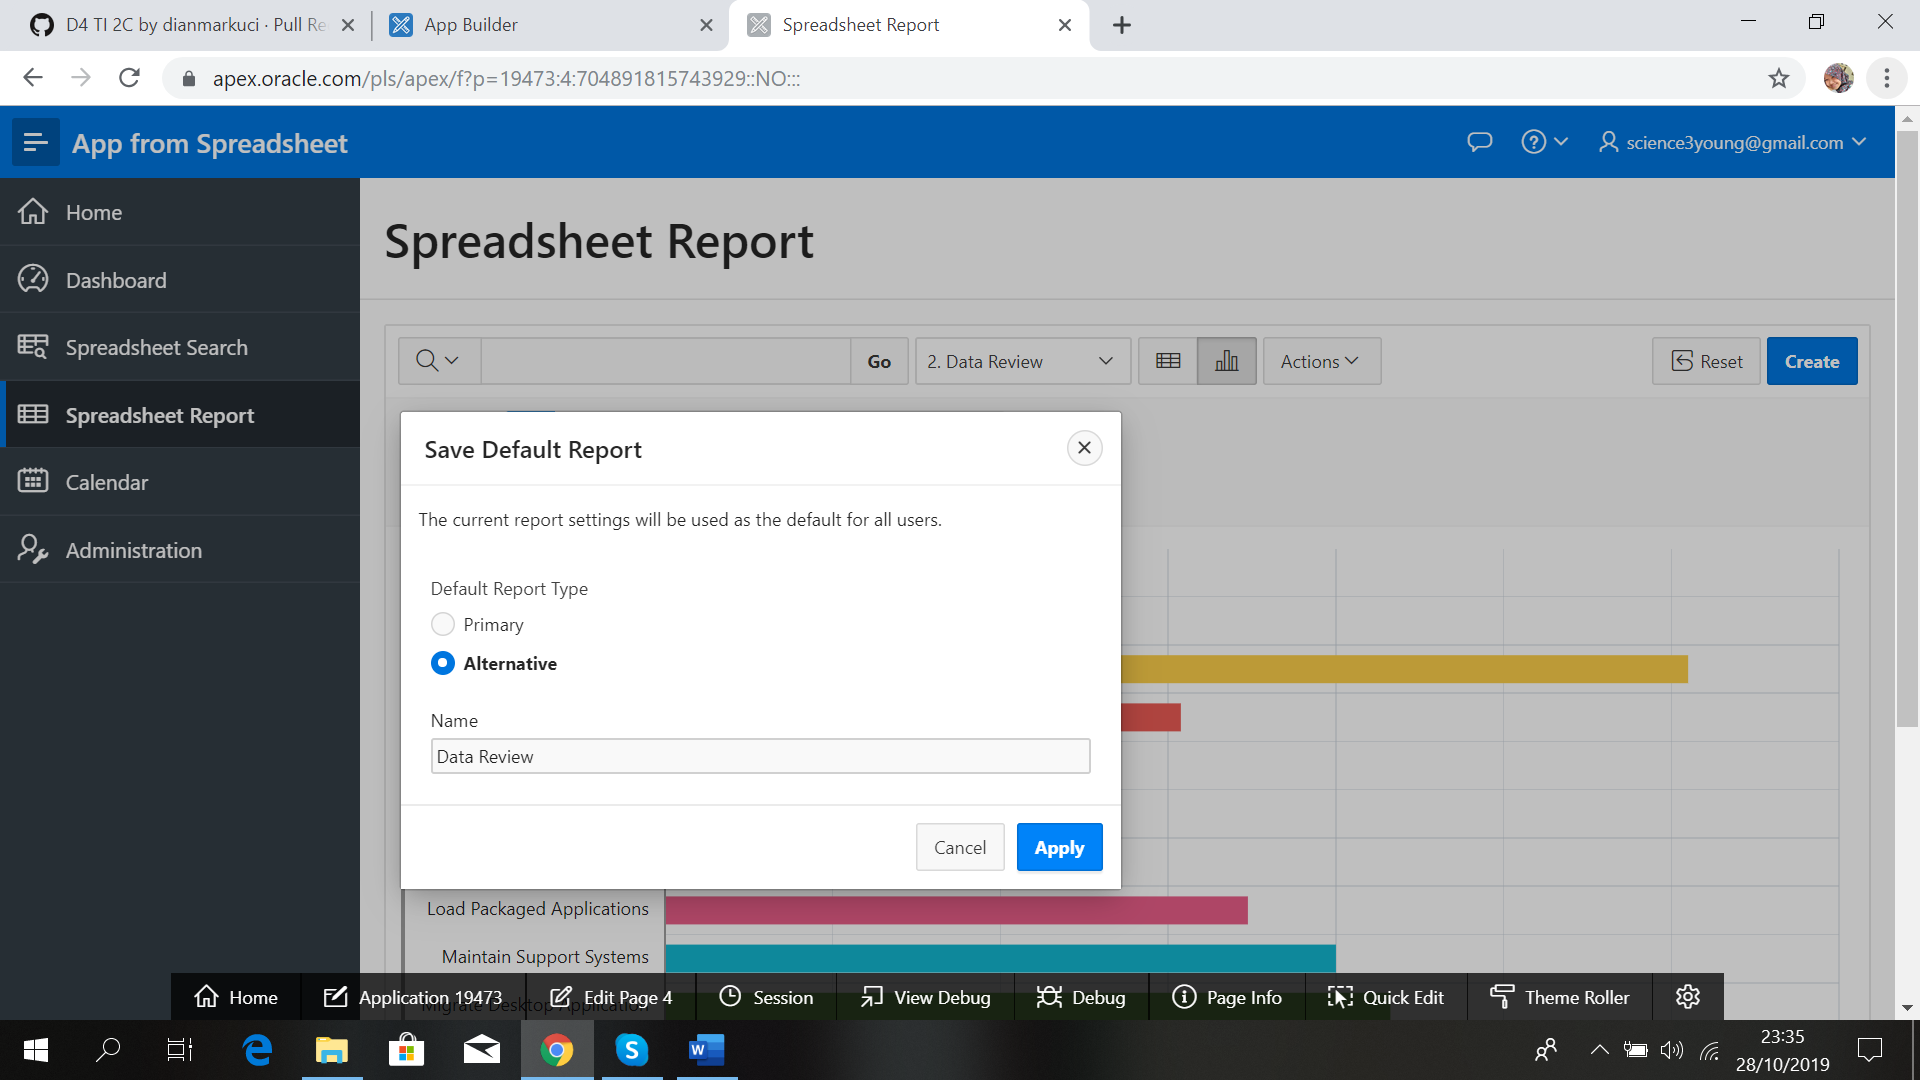
\includegraphics[width=10cm\textwidth]{figure/26.png}
\end{center}

\item 14. Membatasi status
\begin{center}
     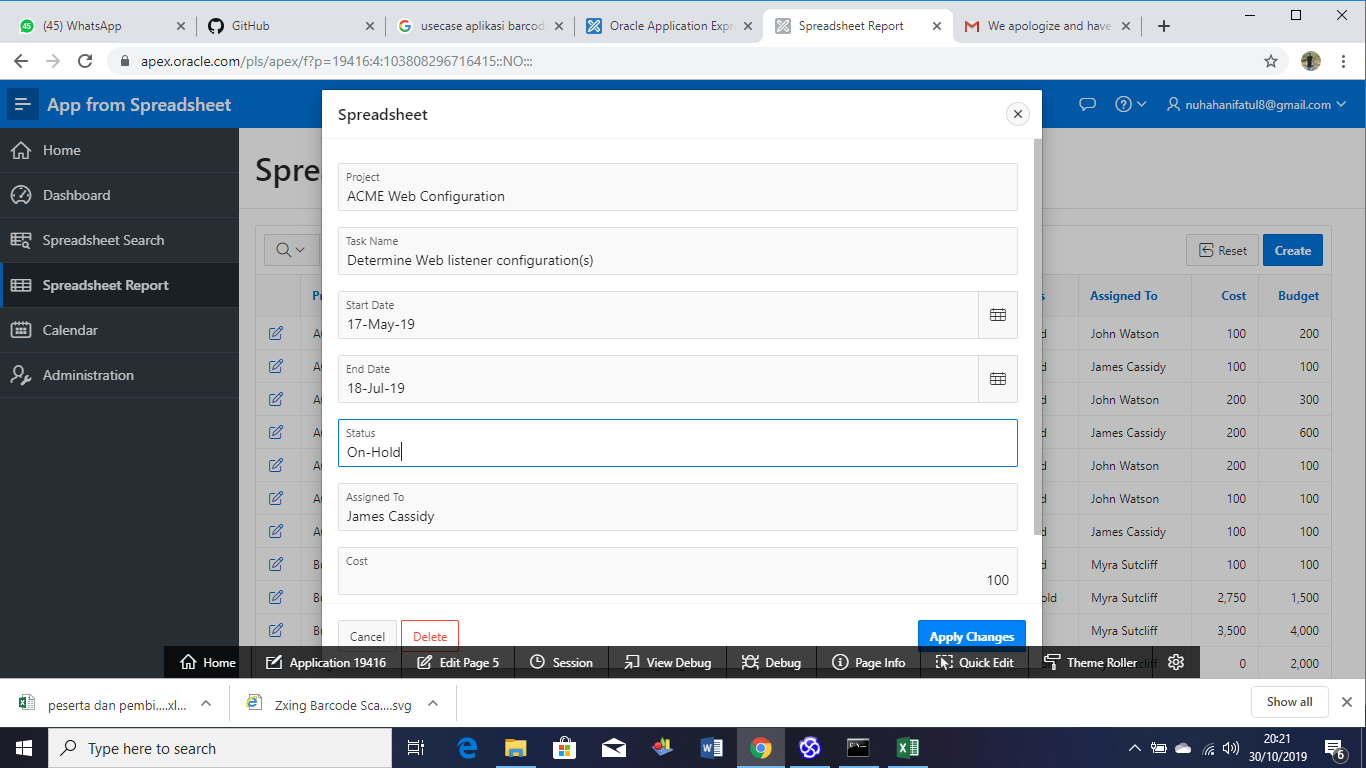
\includegraphics[width=10cm\textwidth]{figure/29.png}
\end{center}

\item 15. Quick Edit pada status
\begin{center}
    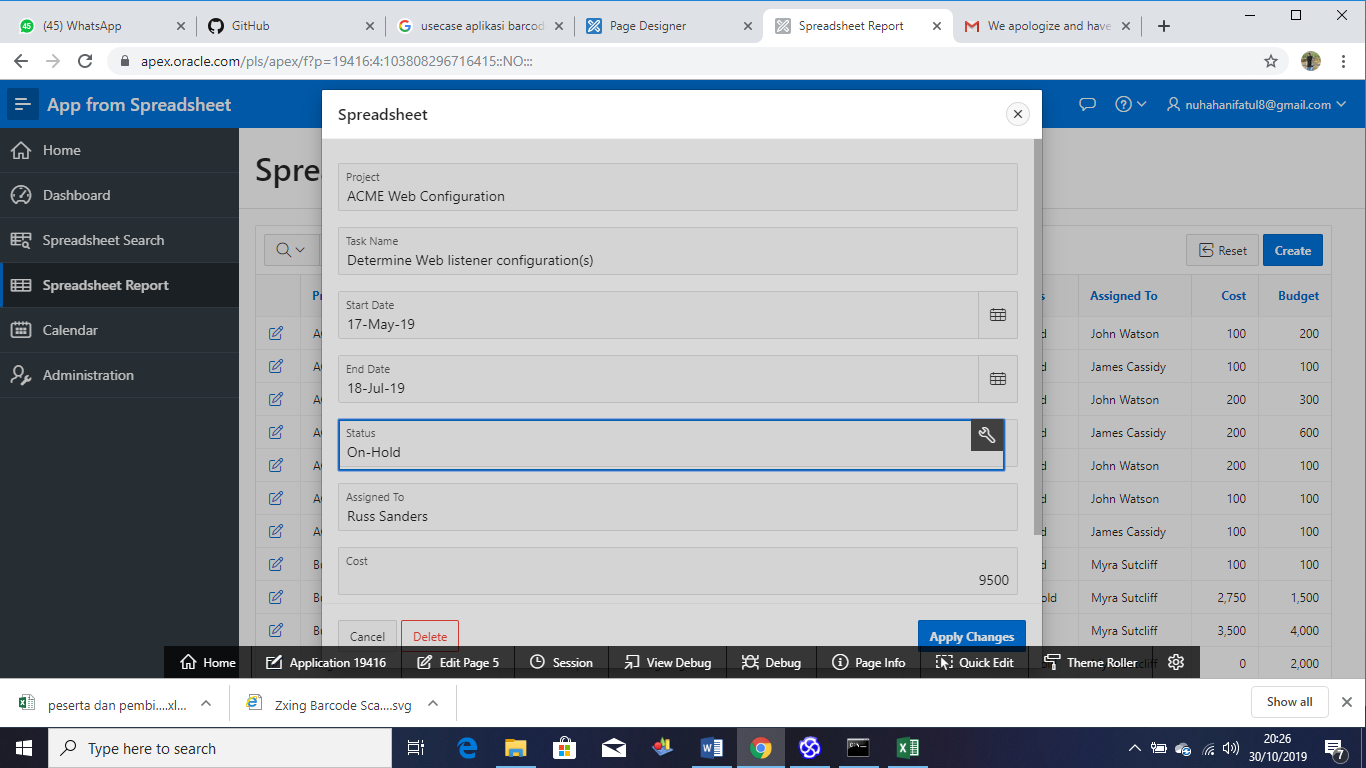
\includegraphics[width=10cm\textwidth]{figure/30.png}
\end{center}

\item 16. Setelah quick edit akan muncul ini dan  Pada identification type pilih select list

\begin{center}
    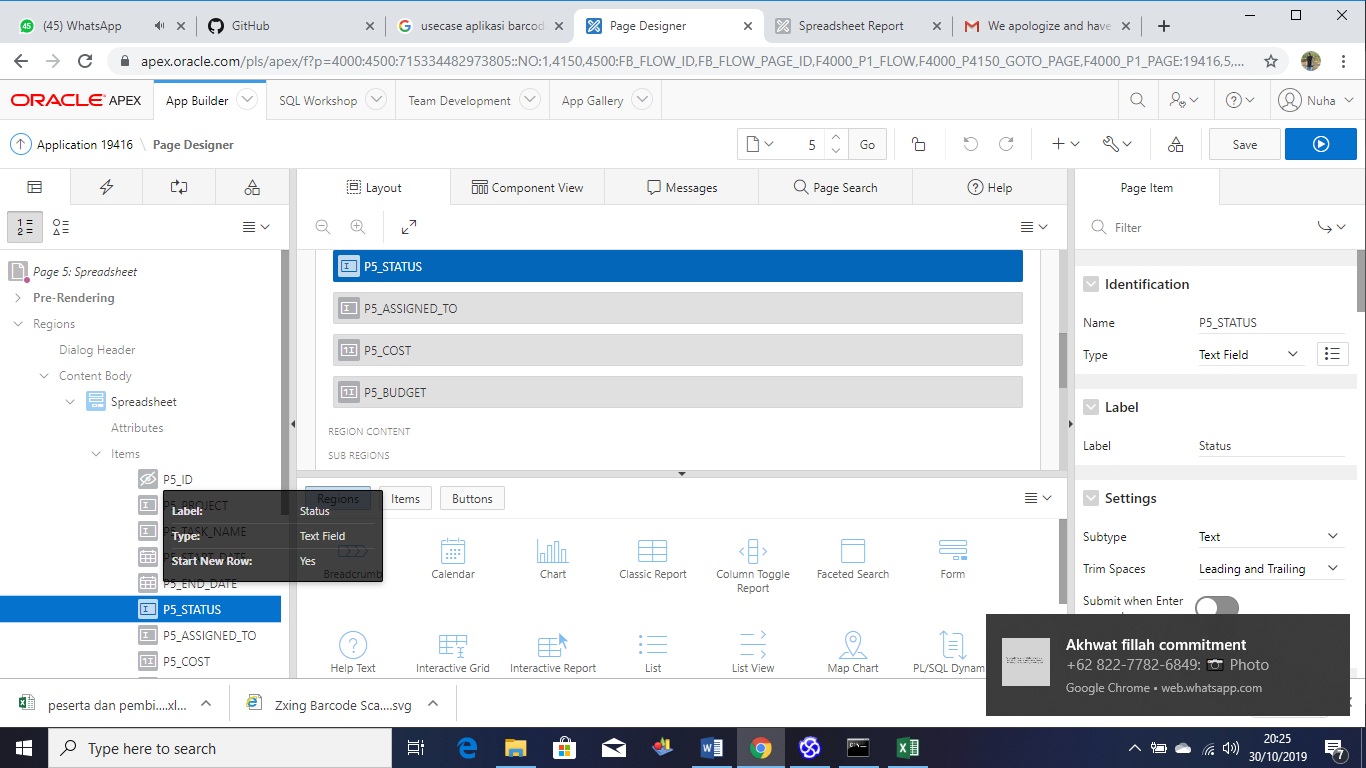
\includegraphics[width=10cm\textwidth]{figure/31.png}
    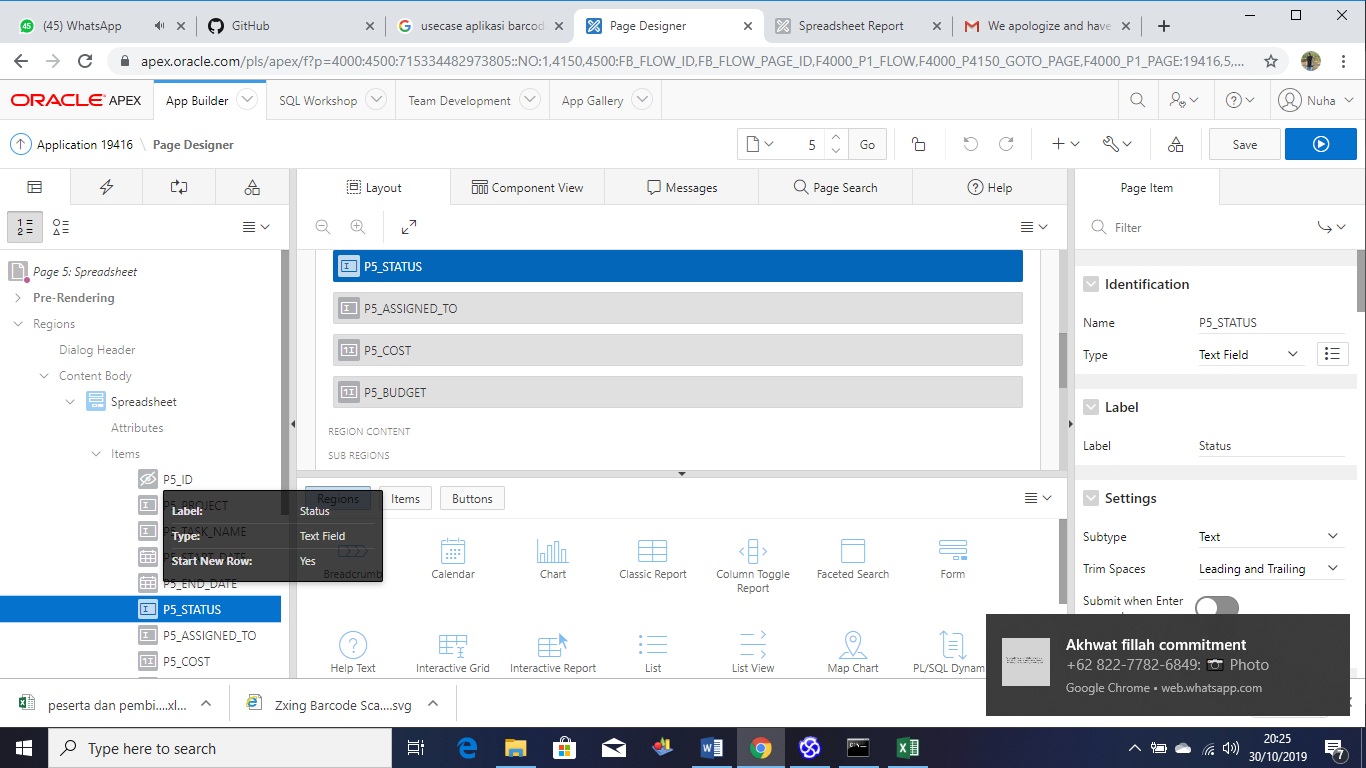
\includegraphics[width=10cm\textwidth]{figure/32.png}
\end{center}


\item 18. Scroll ke bawah pada list of values pilih  SQL Quary
\begin{center}
    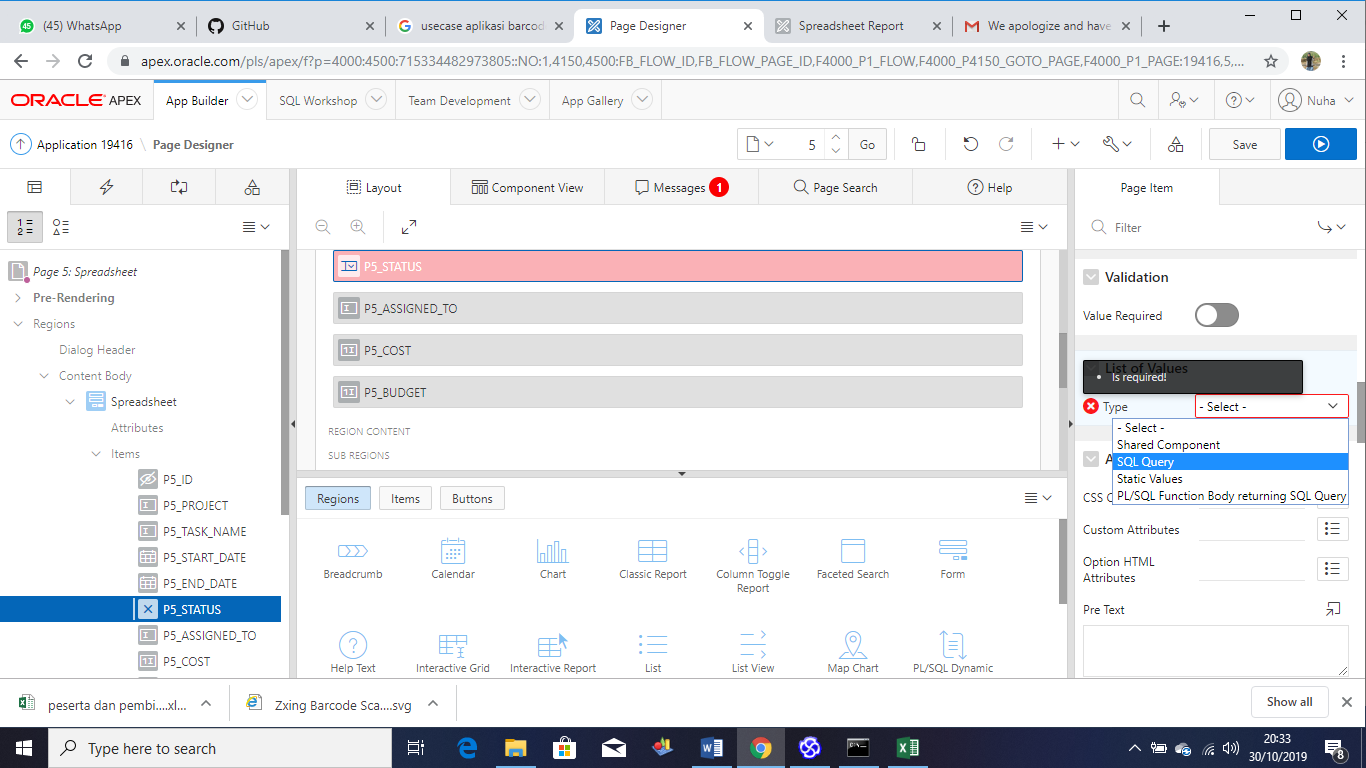
\includegraphics[width=10cm\textwidth]{figure/34.png}
\end{center}

\item 19. Pada sql quary pilih code editor
\begin{center}
    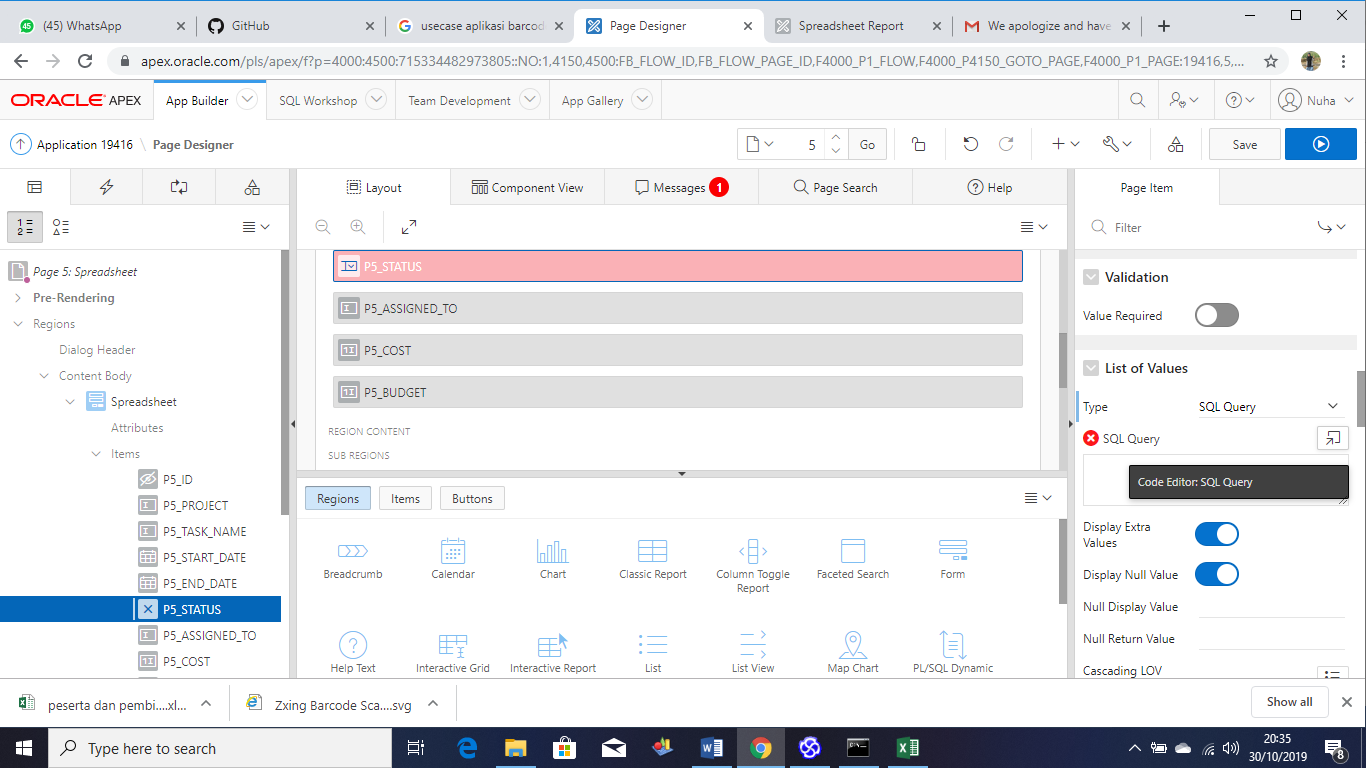
\includegraphics[width=10cm\textwidth]{figure/35.png}
\end{center}

\item 20.Pada identification type pilih select list

\begin{center}
    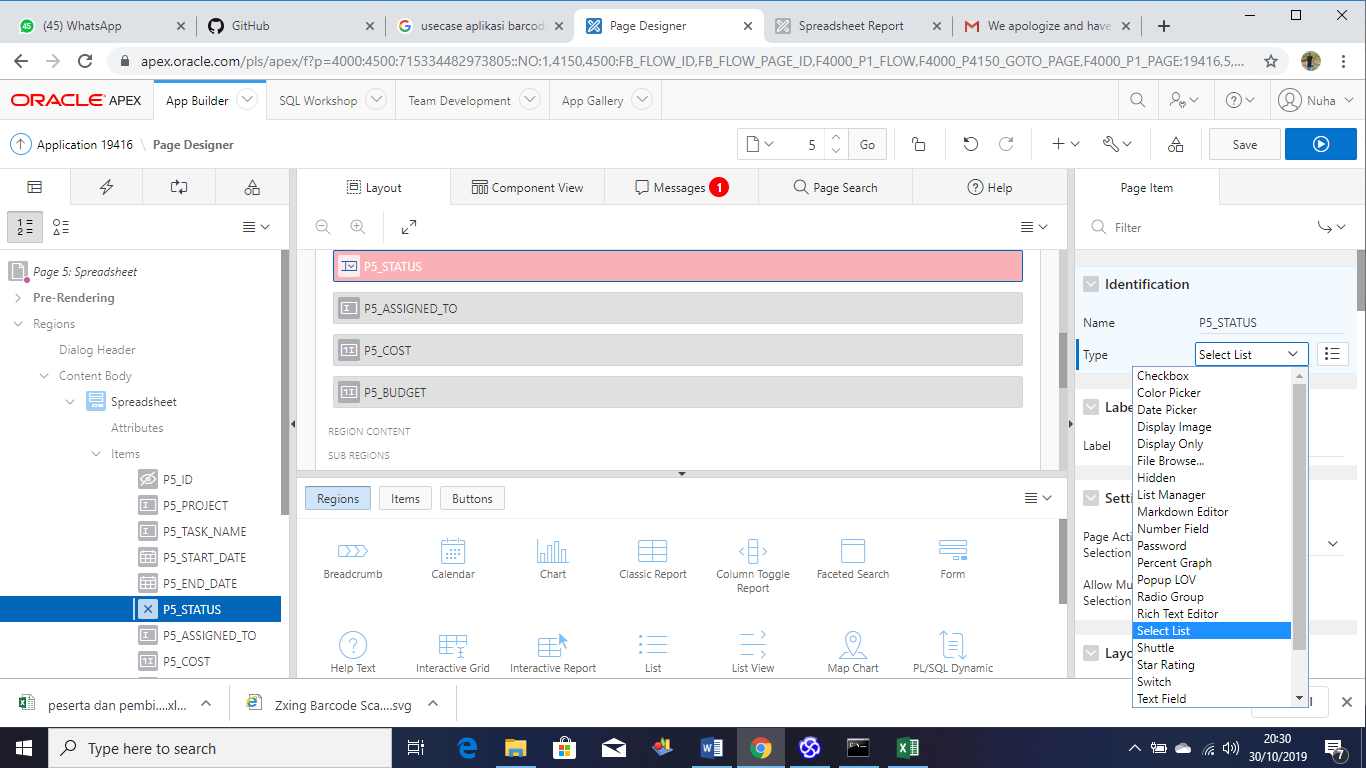
\includegraphics[width=10cm\textwidth]{figure/33.png}
\end{center}

\item 21.  Scroll ke bawah pada list of values pilih  SQL Quary
\begin{center}
    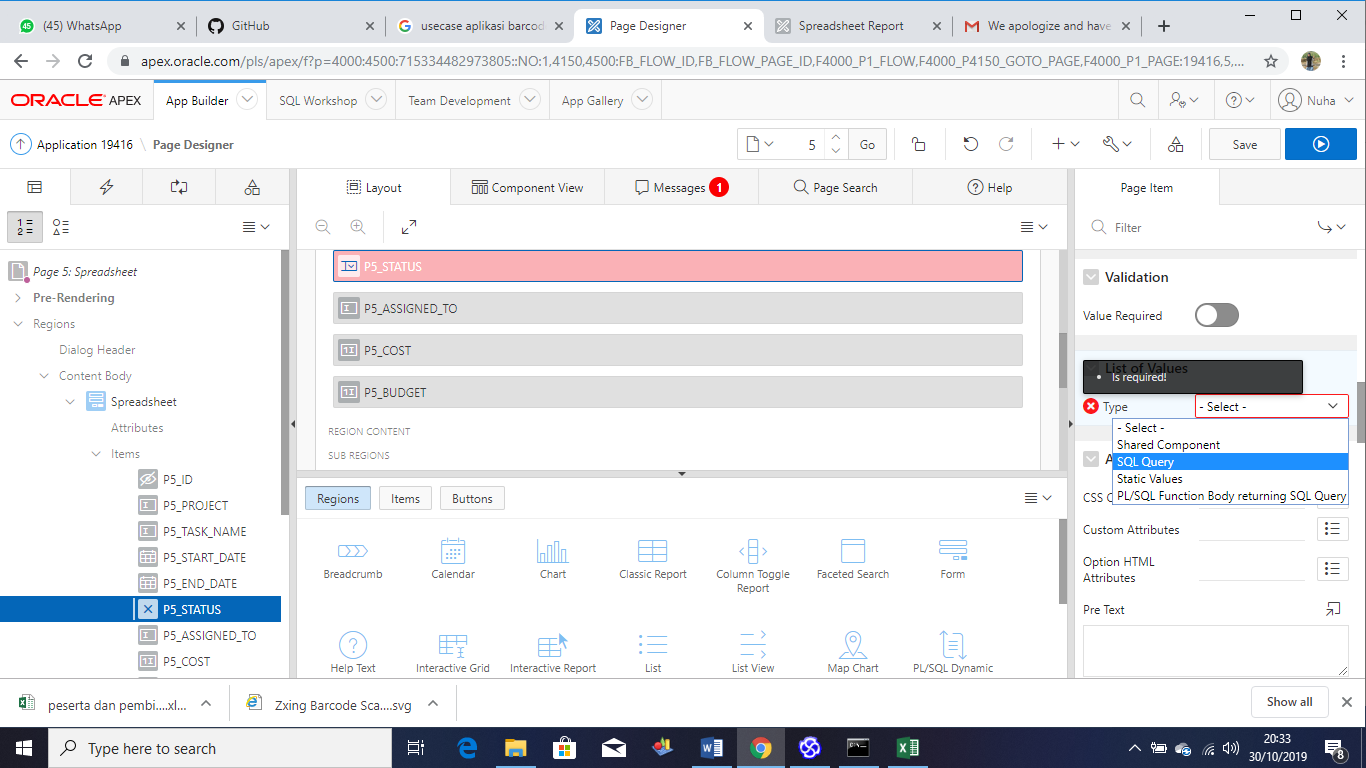
\includegraphics[width=10cm\textwidth]{figure/34.png}
\end{center}

\item 22. Pada code editor ketikkan “select distinct status d, status r from spreadsheet order by 1”
\begin{center}
    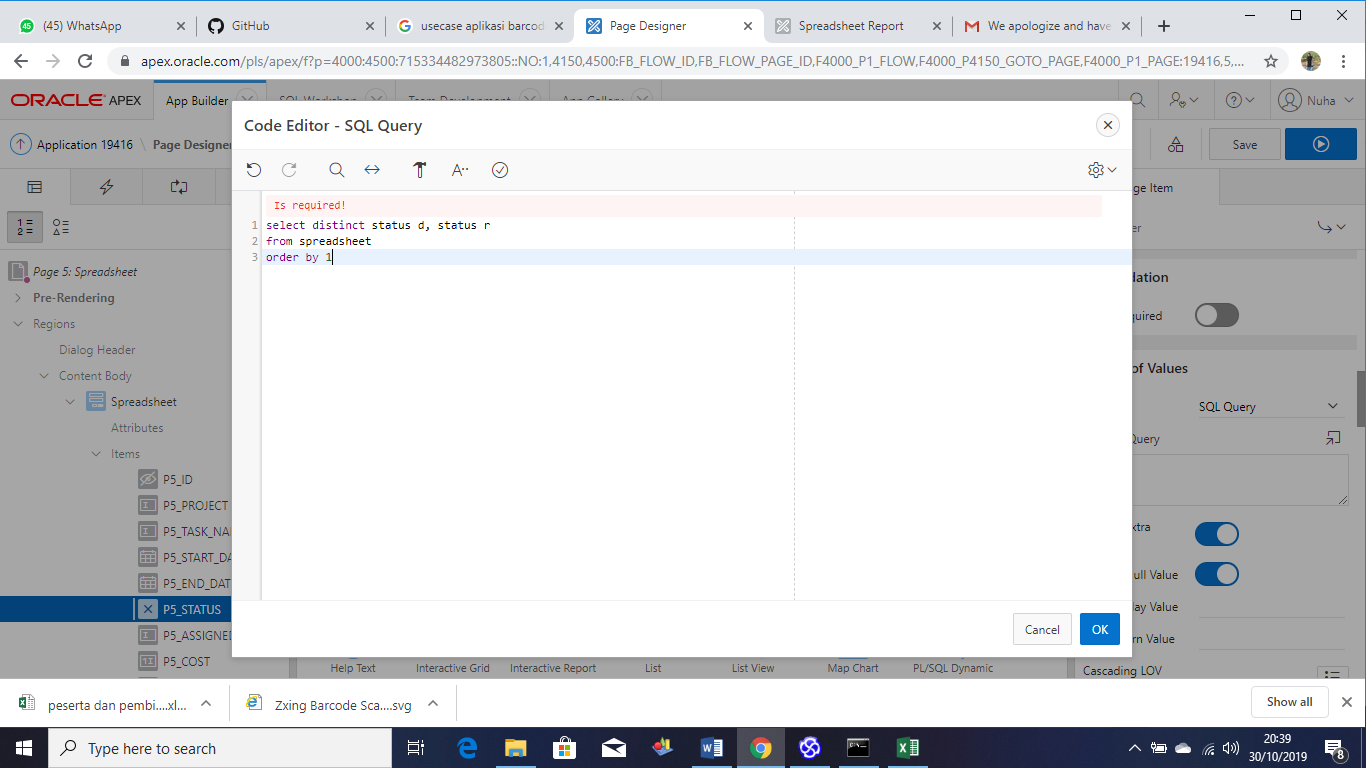
\includegraphics[width=10cm\textwidth]{figure/36.png}
\end{center}

\item 23. Klik validate lalu klik oke
\begin{center}
     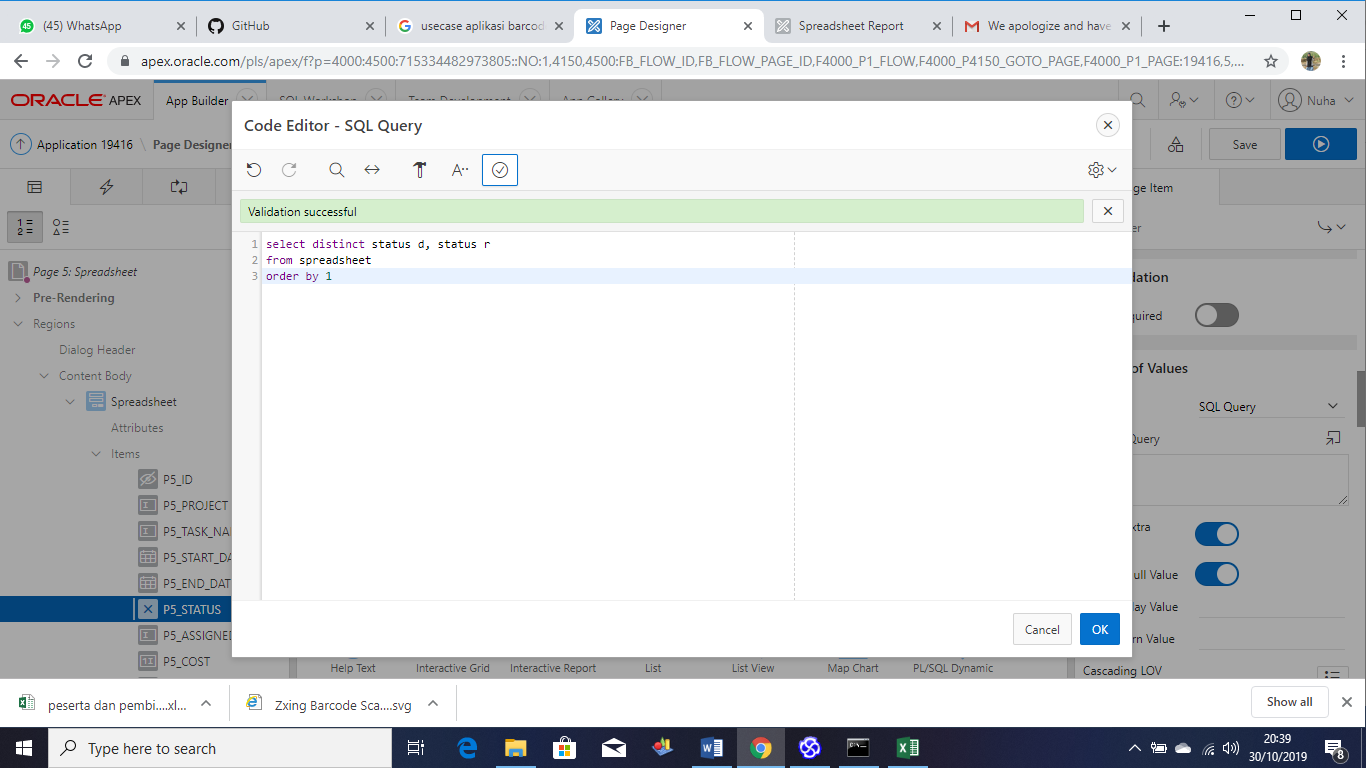
\includegraphics[width=10cm\textwidth]{figure/37.png}
\end{center}





    
    






\end{document}